\documentclass[a4paper,11pt]{book}
% Long footnote URLS
\usepackage[hyphens]{url}

\usepackage{listings}
\usepackage{xspace}
\usepackage[utf8]{inputenc}
\usepackage[spanish]{babel}
\usepackage{pdfpages}
\usepackage{amsmath}
\usepackage[official]{eurosym}

\decimalpoint
\usepackage{dcolumn}
\newcolumntype{.}{D{.}{\esperiod}{-1}}
\makeatletter
\addto\shorthandsspanish{\let\esperiod\es@period@code}
\makeatother

\RequirePackage{verbatim}
\usepackage{fancyhdr}
\usepackage{graphics, graphicx, float}
\usepackage{afterpage}

\usepackage{longtable}

\usepackage[pdfborder={0 0 0}]{hyperref}
\usepackage[printonlyused]{acronym}
\newcommand{\Acro}[2]{\acro{#1}{#2}\acused{#1}}

% ********************************************************************
% Re-usable information
% ********************************************************************
\newcommand{\myTitle}{MineRVa\xspace}
\newcommand{\mySubtitle}{Experiencia de juego en Realidad Virtual en un museo\xspace}
\newcommand{\myEnglishSubtitle}{Virtual museum generator\xspace}
\newcommand{\myDegree}{Máster en Ingeniería Informática\xspace}
\newcommand{\myName}{Pedro Manuel Gómez-Portillo López\xspace}
\newcommand{\myProf}{Francisco Luis Gutiérrez Vela\xspace}
\newcommand{\myFaculty}{Escuela Técnica Superior de Ingenierías Informática y de Telecomunicación\xspace}
\newcommand{\myFacultyShort}{E.T.S. de Ingenierías Informática y de Telecomunicación\xspace}
\newcommand{\myDepartment}{Departamento\xspace}
\newcommand{\myUni}{\protect{Universidad de Granada}\xspace}
\newcommand{\myLocation}{Granada\xspace}
\newcommand{\myTime}{\today\xspace}
\newcommand{\myPalabrasclave}{palabras, clave}
\newcommand{\myKeywords}{key, words}


\hypersetup{
pdfauthor = {\myName (gomezportillo@correo.ugr.es)},
pdftitle = {\myTitle},
pdfsubject = {},
pdfkeywords = {\myKeywords},
pdfproducer = {pdflatex}
}

\usepackage{colortbl,longtable}
\usepackage[stable]{footmisc}

\pagestyle{fancy}
\fancyhf{}
\fancyhead[LO]{\leftmark}
\fancyhead[RE]{\rightmark}
\fancyhead[RO,LE]{\textbf{\thepage}}
\renewcommand{\chaptermark}[1]{\markboth{\textbf{#1}}{}}
\renewcommand{\sectionmark}[1]{\markright{\textbf{\thesection. #1}}}

\setlength{\headheight}{1.5\headheight}

\newcommand*\justify{
	\fontdimen2\font=0.4em
	\fontdimen3\font=0.2em
	\fontdimen4\font=0.1em
	\fontdimen7\font=0.1em
	\hyphenchar\font=`\-
}
\newcommand{\HRule}{\rule{\linewidth}{0.5mm}}

\newcommand{\dedication}[1]{%
  \cleardoublepage
  \thispagestyle{empty}
  \null\vspace{\stretch{1}}
  \begin{flushright}
    \textit{#1}
  \end{flushright}
  \vspace{\stretch{2}}\null
  \cleardoublepage
}

\definecolor{gray97}{gray}{.97}
\definecolor{gray75}{gray}{.75}
\definecolor{gray45}{gray}{.45}
\definecolor{gray30}{gray}{.94}

\lstset{ frame=Ltb,
     framerule=0.5pt,
     aboveskip=0.5cm,
     framextopmargin=3pt,
     framexbottommargin=3pt,
     framexleftmargin=0.1cm,
     framesep=0pt,
     rulesep=.4pt,
     backgroundcolor=\color{gray97},
     rulesepcolor=\color{black},
     stringstyle=\ttfamily,
     showstringspaces = false,
     basicstyle=\scriptsize\ttfamily,
     commentstyle=\color{gray45},
     keywordstyle=\bfseries,
     numbers=left,
     numbersep=6pt,
     numberstyle=\tiny,
     numberfirstline = false,
     breaklines=true,
}

\lstnewenvironment{listing}[1][]
   {\lstset{#1}\pagebreak[0]}{\pagebreak[0]}

\lstdefinestyle{C} {
	basicstyle=\scriptsize,
	frame=single,
	language=C,
	numbers=left
}

\lstdefinestyle{C++} {
	basicstyle=\small,
	frame=single,
	backgroundcolor=\color{gray30},
	language=C++,
	numbers=left
}

\lstdefinestyle{Consola} {
   	basicstyle=\scriptsize\bf\ttfamily,
    backgroundcolor=\color{gray30},
    frame=single,
    language=shell,
    numbers=none
}

\lstdefinestyle{XML} {
	basicstyle=\scriptsize,
	frame=single,
	language=XML,
	numbers=left
}

\newcommand{\bigrule}{\titlerule[0.5mm]}

\makeatletter
\def\clearpage{%
  \ifvmode
    \ifnum \@dbltopnum =\m@ne
      \ifdim \pagetotal <\topskip
        \hbox{}
      \fi
    \fi
  \fi
  \newpage
  \thispagestyle{empty}
  \write\m@ne{}
  \vbox{}
  \penalty -\@Mi
}
\makeatother

\usepackage{pdfpages}


%%------------- ESTILOS PROPIOS ---------------------------
\usepackage{caption}
\captionsetup{justification=centering}

\newcommand{\MineRVa}{\textit{MineRVa} }
\renewcommand*{\lstlistlistingname}{Índice de listados}
\renewcommand{\listtablename}{Índice de tablas} %% not working 

\addto\captionsenglish{\renewcommand{\appendixname}{Apéndices}}

\newcommand{\appendixtitle} {
  \cleardoublepage
%  \thispagestyle{empty}
  \vspace*{5cm}
  \begin{center}
    \sffamily\scshape\Large\scalebox{3}{APÉNDICES}
  \end{center}
}

\usepackage{csquotes}
\usepackage{eurosym}

%% -- letras capitales
\usepackage{lettrine}
\newcommand{\drop}[2]{
  \lettrine[lines=2]
  {\textcolor[gray]{0.4}{\textbf{#1}}}{#2}
  }

% Cajas grises
\usepackage{tcolorbox}

%%---------------------------------------------------------


\begin{document}
\begin{titlepage}
 
\newlength{\centeroffset}
\setlength{\centeroffset}{-0.5\oddsidemargin}
\addtolength{\centeroffset}{0.5\evensidemargin}
\thispagestyle{empty}

\noindent\hspace*{\centeroffset}
\begin{minipage}{\textwidth}
\centering

\includegraphics[width=0.9\textwidth]{imagenes/misc/ugr}\\[1.4cm]
\textsc{ \Large TRABAJO FIN DE MÁSTER\\[0.2cm]}
\textsc{ MÁSTER EN INGENIERÍA INFORMÁTICA}\\[1cm]
{\Huge\bfseries \myTitle \\}
\noindent\rule[-1ex]{\textwidth}{3pt}\\[3.5ex]
{\large\bfseries \mySubtitle}
\end{minipage}

\vspace{2.5cm}

\noindent\hspace*{\centeroffset}
\begin{minipage}{\textwidth}
\centering
\textbf{Autor}\\ {\myName}\\[2.5ex]
\textbf{Director}\\ {\myProf}\\[2cm]

\includegraphics[width=0.3\textwidth]{imagenes/misc/etsiit}\\[0.1cm]
\textsc{\myFaculty}\\
\textsc{---}\\
\myLocation, \myTime
\end{minipage}

\end{titlepage}



\chapter*{}

\begin{titlepage}
 
 
\setlength{\centeroffset}{-0.5\oddsidemargin}
\addtolength{\centeroffset}{0.5\evensidemargin}
\thispagestyle{empty}

\noindent\hspace*{\centeroffset}
\begin{minipage}{\textwidth}
\centering
\vspace{3.3cm}
%\includegraphics[width=3cm]{imagenes/logo} 
\vspace{0.5cm}

{\Huge\bfseries \myTitle \\}
\noindent\rule[-1ex]{\textwidth}{3pt}\\[3.5ex]
{\large\bfseries \mySubtitle \\[4cm]}
\end{minipage}

\vspace{2.5cm}

\noindent\hspace*{\centeroffset}
\begin{minipage}{\textwidth}
\centering
\textbf{Autor}\\ {\myName}\\[2.5ex]
\textbf{Director}\\ {\myProf}\\[2cm]
\end{minipage}

\vspace{\stretch{2}}

\end{titlepage}




\cleardoublepage
\thispagestyle{empty}

\copyrightpage

\begin{center}
{\large\bfseries \myTitle: \mySubtitle}\\
\end{center}

\begin{center}
\myName \\
\end{center}

\vspace{0.7cm}
\noindent{\textbf{Palabras clave}: \myPalabrasclave }\\

\vspace{0.7cm}
\noindent{\textbf{Resumen}}\\

% Resumen
Las tecnologías asociada a la Realidad Virtual permiten que personas que no pueden acceder a centros, como puede ser un museo, puedan visitarlo de una forma más o menos realista y en muchos casos incluso motivadora por la tecnología que se emplea.

\thispagestyle{empty}

\cleardoublepage

\begin{center}
	{\large\bfseries \myTitle: \myEnglishSubtitle}\\
\end{center}

\begin{center}
	\myName \\
\end{center}

\vspace{0.7cm}
\noindent{\textbf{Keywords}: \myKeywords }\\

\vspace{0.7cm}
\noindent{\textbf{Abstract}}\\

% Abstract




% \chapter*{}
% \thispagestyle{empty}

% \noindent\rule[-1ex]{\textwidth}{2pt}\\[4.5ex]

% Yo, \textbf{\myName}, alumno de la titulación \myDegree de la \textbf{\myFaculty}, con DNI 71722388Q, autorizo la ubicación de la siguiente copia de mi Trabajo Fin de Máster en la biblioteca del centro para que pueda ser consultada por las personas que lo deseen.

% \vspace{6cm}

% \noindent Fdo: \myName

% \vspace{2cm}

% \begin{flushright}
% \myLocation a \myTime.
% \end{flushright}


\chapter*{}
\thispagestyle{empty}

\noindent\rule[-1ex]{\textwidth}{2pt}\\[4.5ex]

D. \textbf{\myProf}, Profesor del \myDepartment de la \myUni.

\vspace{0.5cm}

\textbf{Informa:}

\vspace{0.5cm}

Que el presente trabajo, titulado \textit{\textbf{\myTitle, \mySubtitle}}, ha sido realizado bajo su supervisión por \textbf{\myName}, y autoriza la defensa de dicho trabajo ante el tribunal que corresponda.

\vspace{0.5cm}

Y para que conste, expide y firma el presente informe en \myLocation a \myTime.

\vspace{1cm}

\textbf{El director:}

\vspace{5cm}

\noindent \textbf{\myProf}


\dedication{A mi historiadora del arte}

\frontmatter
\tableofcontents
\listoffigures
\listoftables
\lstlistoflistings
\chapter{Lista de acrónimos}
{
\small
\begin{acronym}[XXXXXXXX]

\acro{IDE}     {Integrated Development Environment}
\acro{TFM}     {Trabajo Final de Máster}
\acro{VR}      {Virtual Reality}
\acro{VRTK}    {Virtual Reality Toolkit}
\acro{GDD}     {Game Design Document}


\acro{CSS}     {Cascading Style Sheets}
\acro{FPS}     {Frames Per Second}
\acro{GPU}     {Graphical Processing Unit}
\acro{GUI}     {Graphical User Interface}  
\acro{HCI}     {Human-Computer Interaction}
\acro{HTML5}   {Hypertext Markup Language, version 5}
\acro{HTTP}    {Hypertext Transfer Protocol}  
\acro{JPEG}    {Joint Photographic Experts Group}
\acro{JS}      {JavaScript}
\acro{KISS}    {Keep it simple, stupid!} 
\acro{RTS}     {Real Time System}
\acro{RUP}     {Rational Unified Process}
\acro{SDK}     {Software Development Kit}
\acro{TCP}     {Transmission Control Protocol}  
\acro{UPD}     {Unified Process Development}

\end{acronym}
}


% \ac{OO}   la primera vez \acf, después \acs
% \acs{OO}  short: OO
% \acf{OO}  full : Object Oriented (OO)
% \acl{OO}  large: Object Oriented
% \acx{OO}         OO (Object Oriented)

% usa \Acro cuando no debe aparecer nunca expandido en el texto

% Local variables:
%   TeX-master: "main.tex"
% End:


\mainmatter
\setlength{\parskip}{8pt}

\chapter{Introducción}
\label{chap:introduccion}

\drop{S}{  olamente} en 2018, el \textbf{Museo Reina Sofía} de Madrid recibió 3,9 millones de visitantes, aproximadamente un 2\% más que el año anterior. Del mismo modo, el \textbf{Museo de Prado} recibió casi 3 millones, un 2,4\% más que en 2017. Otro ejemplo de esto es el Macba, el Museo de Arte Contemporáneo de Barcelona, que recibió en 2018 casi 332,000 visitantes, un 28\% más que el año anterior\footnote{\url{https://www.abc.es/cultura/arte/abci-museos-espanoles-crecen-2018-201901021635_noticia.html}}. Con estos datos, puede verse que el interés por los museos está creciendo cada vez más.

Pero la industrias de ocio que indiscutible más dinero genera es la \textbf{industria de videojuegos}, que solo en 2018 generó 43 mil millones de dólares, un 18\% más que en 2017\footnote{\url{https://tcrn.ch/2HtFczS}}. Por dar un contexto de estas cifras, en 2016 la suma conjunta del cine y la música en el mundo \textit{solo} generó 815 millones de dólares\footnote{\url{https://www.elperiodico.com/es/ocio-y-cultura/20180827/videojuegos-cine-musica-cultura-comparativa-7001883}}.

Dado el éxito global de esta industrial, han comenzado a nacer nuevas maneras de jugar y nuevas técnicas de interacción con los usuarios, como la \textbf{Realidad Virtual}. La Realidad Virtual es un paradigma de interacción que intenta ofrecer a sus jugadores una experiencia lo más \textbf{inmersiva} posible, para lo que hace uso de la visión estereoscópica de las personas para hacerles creer que el mundo real es lo que ven, y no solo una pantalla.

Además, los dispositivos que permiten hacer uso de estas tecnologías se están abaratando cada vez más, hasta el punto de que un jugador casual puede permitirse adquirir un headset \acs{VR} para utilizarlo esporádicamente, en lugar de ser una tecnología que solo se plantena comprar aquellos que creen que le van a dar mucho uso.

\section{Motivación del proyecto}

El principal objetivo a la hora de integrar videojuegos y tecnologías de Realidad Virtual en este proyecto es el poder crear respectivamente entornos interactivos e inmersivos que, unidos al potencial motivador que tienen de manera intrínseca los videojuegos, consigan animar a los usuarios que disfruten de \MineRVa a visitar museos reales y ser, principalmente para aquellos que no puedan hacerlo por razones físicas, un sustituto que les permita disfrutar en la medida de lo posible de ello. 

\section{Motivación personal}

Siempre he estado muy interesado en el desarrollo de videojuegos y en el proceso técnico que hay detrás. Durante el grado, que estudié en la Universidad de Castilla-La Mancha, tuve la suerte de coincidir con algunos profesores que también estaban muy interesados en este tema y que habían organizado dos cursos; el primero, en 2015, fue el \textbf{Curso de Desarrollo de videojuegos multi-plataforma para dispositivos móviles}\footnote{\url{http://www.curso-openfl.cedv.quijost.com/}}, un curso de 100 horas en el que desarrollamos un juego en 2D en Haxe utilizando el framework OpenFL.

Tras él, dos años más tarde completé el \textbf{Curso de Experto en desarrollo de videojuegos}\footnote{\url{http://cedv.es}}, de 750 horas, en el que realizamos varios proyectos en C++ utilizando el motor de gráficos Ogre3D y otras tecnologías como la librería de interfaces CEGUI o el motor de físicas Bullet.

A raíz de estos cursos comencé a interesarme por Blender, un programa de diseño 3D que integra todos los componentes necesarios para modelar, texturizar, animar y renderizar prácticamente cualquier proyectos.

Por un lado, nunca había trabajando con entornos de desarrollo específicos para videojuegos como Unity, y ni mucho menos con tecnologías de Realidad Virtual, lo que me pareció un reto extremadamente interesante. Por otro, aunque ya había trabajado desarrollando sistemas interactivos nunca lo había hecho aplicando metodologías adecuadas y específicas de desarrollo de videojuegos, por lo que este proyecto parecía el contexto perfecto como primera toma de contacto con ellas.

Del mismo modo, siempre me ha interesado mucho la Historia del Arte y he intentado visitar museos siempre que he tenido la oportunidad, por lo que estoy muy motivado al poder integrar ambos en este proyecto.

\section{Entorno}

El entorno de ejecución de \MineRVa está compuesto por unas gafas de Realidad Virtual, dos controladores y un ordenador personal. Por tanto, el programa final debe ser lo suficientemente ligero y eficiente en cuanto a recursos para poder ser ejecutado en un ordenador que no sea especialmente potente.

La figura \ref{fig:entorno}, renderizada en Blender, presenta un ejemplo de ejecución en el que se puede ver a un usuario llevando puestos el headset \acs{VR} y los mandos mientras juega en uno de las escenarios iniciales. 

\begin{figure}[!h]
\vspace{0.4cm}
\begin{center}
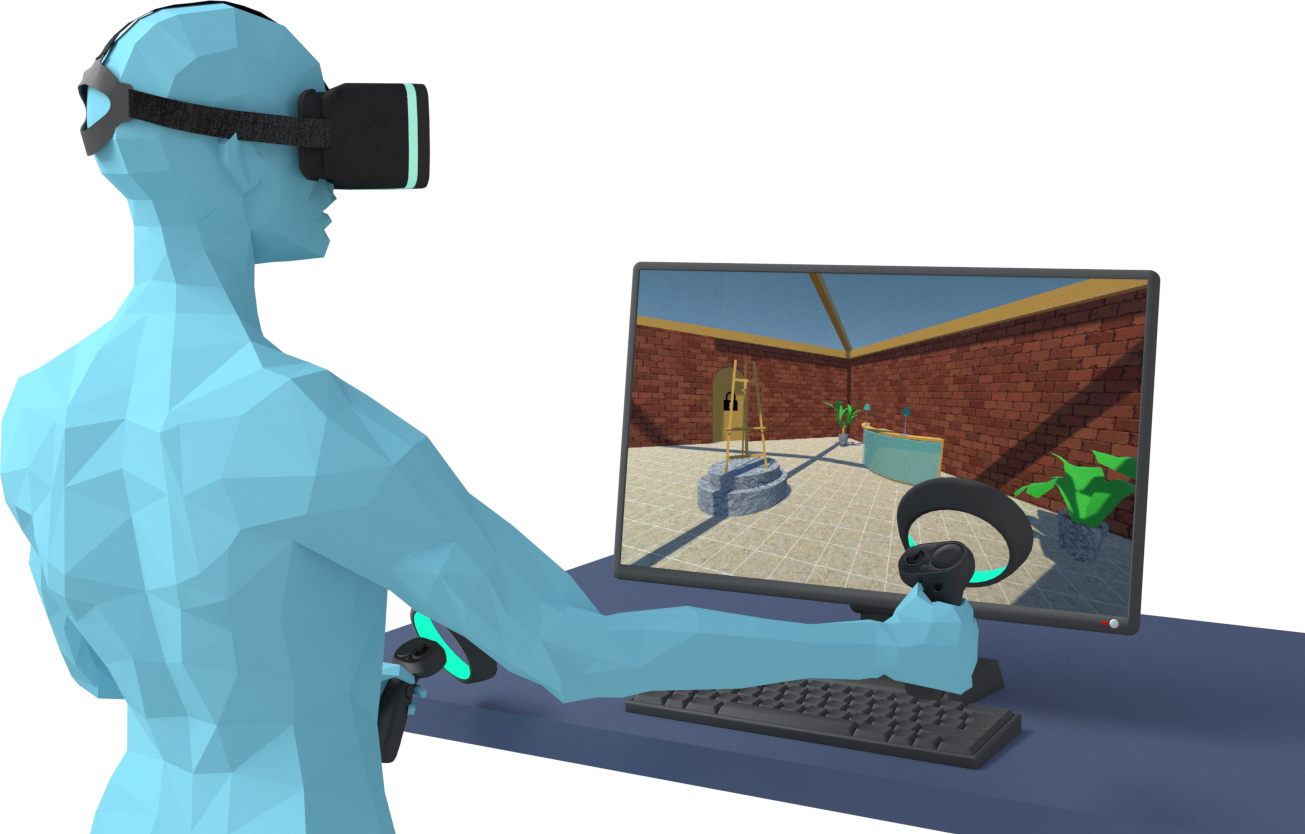
\includegraphics[width=1\textwidth]{imagenes/1/entorno-diffuse-2.png}
\caption{Diagrama de entorno de \MineRVa}
\label{fig:entorno}
\end{center}
\end{figure}

Además, como en este juego no es necesario hacer movimientos rápidos y bruscos, no es necesario contar con mucho espacio libre alrededor del jugador, lo que lo hace aún más accesible al público en general, que no tendrá que disponer de una sala amplia específica para utilizar tecnologías \acs{VR}.


\section{Objetivos}

\subsection{Objetivo principal}

El objetivo de \MineRVa es crear una experiencia inmersiva en la que el jugador se sienta gratificado al ir resolviendo los pequeños acertijos que se le proponen. Con ello se pretende alcanzar dos objetivos diferentes; por un lado, se busca conseguir que nativos digitales que no suelan visitar museos encuentren en \MineRVa una excusa para hacerlo de manera divertida, y por el otro que usuarios más mayores a los que les gusta visitarlos encuentre en la temática de este proyecto una excusa para jugarlo y disfrutar de la misma forma. En cualquiera de los dos casos se espera que, tras completar el juego, la mayoría de usuarios se interesen en visitar museos reales.

Por otro lado, uno de los nichos de jugadores más pequeños y a la vez uno en el que más se ha pensado es en aquellas personas con movilidad reducida que físicamente no pueden visitar museos. Se espera ayudar especialmente a este colectivo consiguiendo una experiencia equivalente en la medida de lo posible, además de intentar hacerla más amena y motivadora enmarcándola en el contexto de un videojuego.

\subsection{Objetivos secundarios}

Como objetivos secundarios, de naturaleza más personal, se presenta el aprender a desarrollar programas basados en tecnologías de Realidad Virtual, así como a elegir y configurar un entorno adecuado para ello.

Además, al estudiar metodologías de desarrollo de videojuegos reales se espera obtener un mejor conocimiento de cómo funciona el desarrollo de un proyecto de estas características.

\section{Estructura del documento}

Este documento ha sido estructurado siguiendo la normativa de \acs{TFM} de la Escuela Técnica Superior de Ingenierías Informática y de Telecomunicación de la Universidad de Granada a través de los siguientes capítulos.

\subsubsection{Capítulo \ref{chap:estado_arte}. \nameref{chap:estado_arte}}

En este capítulo se realiza una presentación del estado actual de las áreas tratadas en este \acs{TFM}, recopilando y exponiendo información relevante relacionada con la Realidad Virtual o el Desarrollo de Videojuegos, entre otros.

\subsubsection{Capítulo \ref{chap:analisis_problema}. \nameref{chap:analisis_problema}}

En este capítulo se introduce este proyecto y se hablará de la concepción inicial y de la narrativa de \textit{MineRVa}.

\subsubsection{Capítulo \ref{chap:tecnologia}. \nameref{chap:tecnologia}}

Este capítulo recoge los recursos tanto hardware como software que se han utilizado para el desarrollo y documentación de este proyecto.

\subsubsection{Capítulo \ref{chap:metodologias}. \nameref{chap:metodologias}}

A lo largo de este capítulo se hablará de las metodologías de desarrollo de videojuegos y se presentarán las metodologías de trabajo y desarrollo seguidas a lo largo de este proyecto.

\subsubsection{Capítulo \ref{chap:plan_entregas}. \nameref{chap:plan_entregas}}

En este capítulo se presenta y detalla el plan de entregas llevado a cabo al inicio del proyecto para poder cumplir con el plazo de tiempo de entrega.

\subsubsection{Capítulo \ref{chap:desarrollo}. \nameref{chap:desarrollo}}

A lo largo de esta capítulo se presenta el trabajo realizado en el marco del plan de entregas del proyecto, además de los resultados obtenidos y los principales problemas encontrados.

\subsubsection{Capítulo \ref{chap:conclusiones}. \nameref{chap:conclusiones}}

En este capítulo se presenta el resultado final del proyecto, las conclusiones extraídas de su desarrollo y se proponen unas líneas de trabajo futuro para continuar con este proyecto.
\chapter{Estado del arte}
\label{chap:estado_arte}

\drop{E}{  n} este capítulo se presentarán y describirán las principales áreas en las que este \acs{TFM} se ha basado; \textbf{Historia del Arte}, \textbf{Realidad Virtual}, \textbf{Diseño 3D} y \textbf{Desarrollo de Videojuegos}.

Uno de los retos que ha supuesto este proyecto ha sido el de estudiar y comparar las diferentes alternativas que se presentaban a la hora de resolver un determinado problema; por ello, en los casos en los que esto aplique se presentarán las diferentes opciones disponibles que han sido estudiadas.

La descripción de estado del arte de cada una de las áreas en las que se ha basado este trabajo comenzará con un recorrido general a lo largo de su historia, hablando de sus contribuciones y posibilidades para terminar presentando su estado actual. Por ello, el estudio de cada una de las áreas mencionadas se dividirá y se detallará a través de sus subáreas, lo que permitirá un estudio más profundo y más detallado de la misma.

La sección de la \textbf{Historia del Arte} comenzará exponiendo un breve recorrido por sus diferentes etapas de manera crónica. Además, se explicará el origen del nombre de este \acs{TFM}.

A continuación, en la sección de la \textbf{Realidad Virtual} se hablará de su historia, las tecnologías y recursos software disponibles y de las interfaces con las que pueden interactuar los usuarios de esta tecnología.

La siguiente sección hablará del \textbf{Diseño 3D}, de qué programas y suites existen actualmente para modelar tridimensionalmente y qué \acs{IDE}s hay disponibles para desarrollar e implementar sistemas interactivos.

Por último, se hablará del \textbf{Desarrollo de Videojuegos} y de sus aplicaciones en este proyecto desde un punto de vista teórico.

La figura \ref{fig:mapa-conceptual} ofrece un resumen de las diferentes tecnologías que colaboran en \MineRVa y de las relaciones que hay entre ellas.

\vspace{0.4cm}

\begin{figure}[!h]
    \begin{center}
        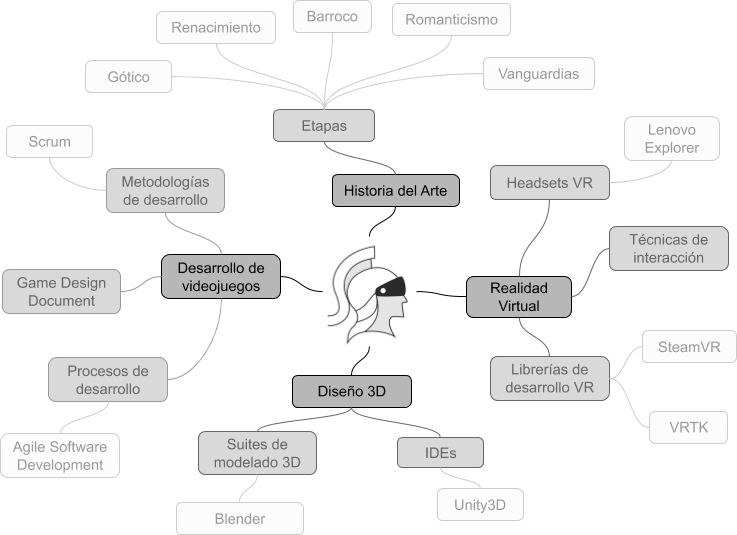
\includegraphics[width=1\textwidth]{imagenes/2/mapa-conceptual.png}
        \caption{Mapa conceptual de \MineRVa}
        \label{fig:mapa-conceptual}
    \end{center}
\end{figure}

\section{Historia del Arte}

Para entender el contexto artístico de este \acs{TFM} primero se presentará un breve resumen a través de las etapas del Arte \cite{ramirez-0610}.

\subsection{Prehistórico}

Habría que remontarse a la etapa prehistórica más antigua, el \textbf{Paleolítico}, para encontrar las primeras muestras de arte. Los primeros homínidos plasmaron su realidad en las paredes de las cuevas y abrigos que habitaron, legándonos lo que hoy conocemos con el nombre de \textbf{pinturas rupestres}. Sirviéndose de pigmentos naturales, grasa animal, carbón y sangre, representaron grupos humanos danzantes y escenas de cacerías con un sentido mágico y sagrado, al existir la creencia de que favorecían la fertilidad de las mujeres de la tribu o fomentaban la caza. El mismo cometido tenían las toscas estatuillas realizadas en piedra y hueso, que con el tiempo fueron sustituidas por otras más refinadas. Por tanto, lo que hoy catalogamos como producciones artísticas a las que atribuimos un valor estético, no fueron ideadas como tal, sino que cumplían una función concreta como medio para obtener ganancias materiales.

\subsection{Mesopotámico y precolombino}

Será en la antigua región de \textbf{Mesopotamia} donde encontremos el origen de la civilización en los términos en los que hoy la entendemos y un arte más acorde con la concepción actual. Las numerosas culturas que se sucedieron en este reducido punto geográfico levantaron una arquitectura pensada y medida, digna de grandes ingenieros capaces de proyectar edificios de gran envergadura, sus conocidos \textit{zigurats}, figura \ref{fig:zigurat} (antecedentes de las pirámides egipcias), por medio de sistemas de arcos y bóvedas. Las artes plásticas no se quedaron atrás. Hoy en día se conservan restos escultóricos y relieves de gran calidad técnica, que han marcado una etapa tan florida como misteriosa de nuestra historia.

\begin{figure}[!h]
    \begin{center}
    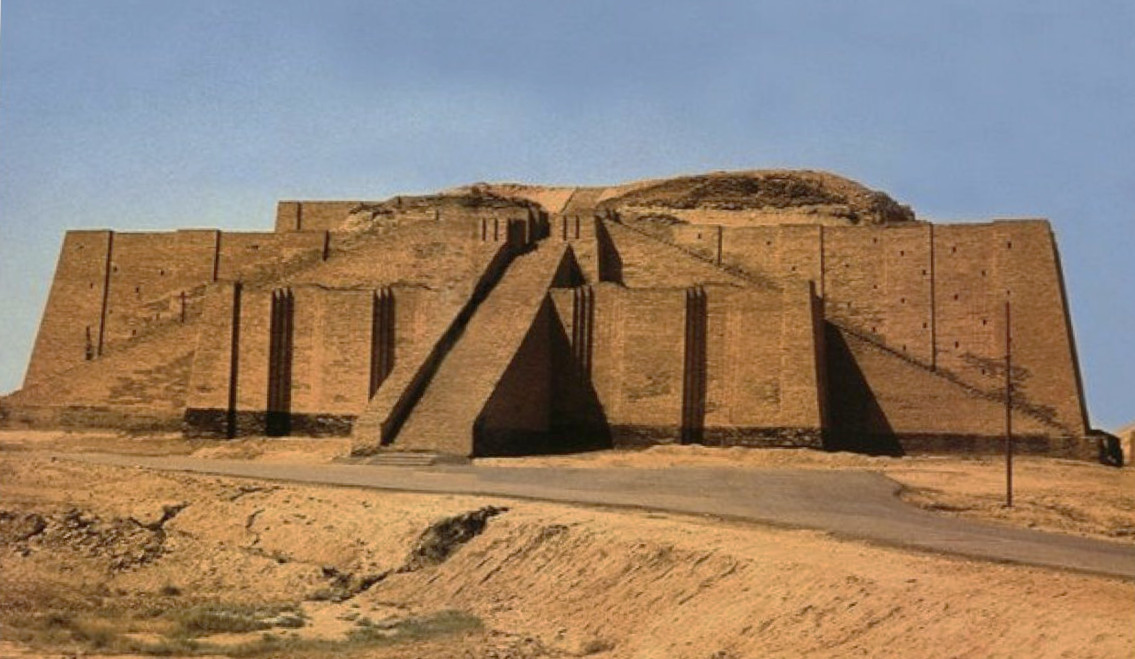
\includegraphics[width=0.7\textwidth]{imagenes/2/zigurat.jpg}
    \caption{\textit{Zigurat} de \textit{Uruk}, 3200-3000 a. C.}
    \label{fig:zigurat}
    \end{center}
\vspace{-0.4cm}
\end{figure}

Paralelamente, cabe destacar la importancia de las manifestaciones artísticas que están teniendo lugar en el continente americano. Los templos \textbf{incas y mayas} son solo un ejemplo del ingenio y la habilidad de aquellas civilizaciones.

\subsection{Arte clásico}

Los \textbf{griegos} abrieron paso a un nuevo tipo de arte basado en la medida humana: la arquitectura está hecha por y para el hombre, y tanto la escultura como la pintura están protagonizadas por la figura humana, en la que reinan los ideales de armonía y proporción. 

Los \textbf{romanos}, muy influenciados por los anteriores, erigieron una arquitectura grandilocuente a la vez que funcional, pensada para el disfrute de los grandes hombres de la época y la exaltación de su poder, igual que los arcos de triunfo y los monumentos conmemorativos. La escultura, heredera de la griega, se vuelve más realista y poderosa.

El nombre de este \acs{TFM} viene de la \textbf{deidad romana Minerva}, que es la \textbf{diosa del arte}, la sabiduría y la guerra, además de la protectora de Roma y la patrona de los artesanos. El poeta Ovidio se refería a Minerva como \textit{la diosa de las mil obras} \cite{lomb-13}. Su equivalente en la mitología griega es Atenea.

\subsection{Arte medieval}

El \textbf{arte islámico} se extendió por Próximo Oriente y avanzó hasta la Península Ibérica, donde los musulmanes permanecieron durante ocho siglos (711-1492). En función de sus zonas de dominio emprendieron un arte muy dispar, centrando sus esfuerzos en la arquitectura especialmente. Fue característico de sus construcciones el uso del arco apuntado, el lobulado y sus variantes, y el arco de herradura, este último sobre todo en la Península dada la influencia visigoda en nuestro territorio. Las yeserías de entramados vegetales, las tracerías, la eboraria y la incorporación del agua y de la naturaleza en la obra artística son otros rasgos distintivos del arte islámico. Ejemplo de ello es el Alcázar de Sevilla, que puede verse en la figura \ref{fig:patio-doncellas}.

\begin{figure}[!h]
    \begin{center}
        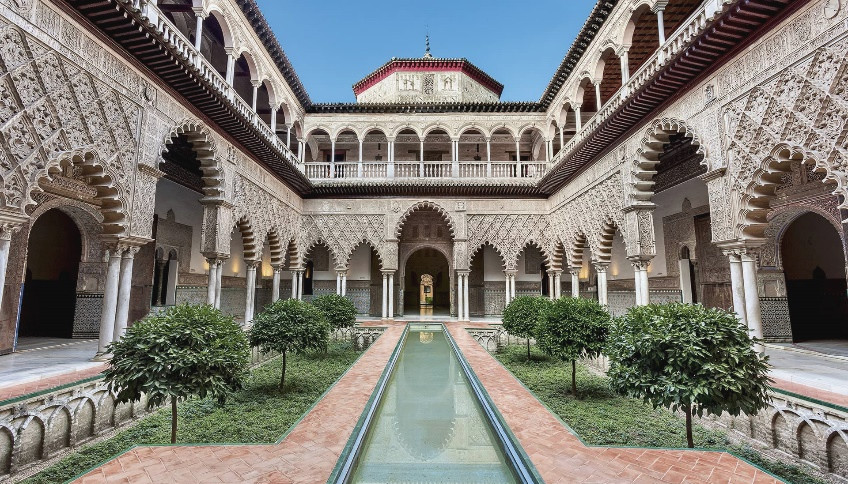
\includegraphics[width=0.7\textwidth]{imagenes/2/patio-doncellas.jpg}
        \caption{Patio de las Doncellas del Alcázar de Sevilla, siglo X}
        \label{fig:patio-doncellas}
    \end{center}
\end{figure}

La llegada de la \textbf{Edad Media} en Europa después de la caída del Imperio Romano de Occidente y la irrupción del cristianismo como nueva religión dominante tuvieron una repercusión directa en el arte generado a partir del siglo V en Europa. La cristiandad encontrará en el \textbf{arte paleocristiano} su primera manifestación, en un principio clandestina, a través de los sarcófagos y pinturas de catacumbas y, tras la legalización de la religión, de manera pública a través de las grandes basílicas. 

Pero fue en el \textbf{románico}, primer estilo internacional de la cultura occidental, donde el cristianismo se manifestó de manera total a partir del siglo X. La arquitectura se caracterizó, en general, por la sencillez estructural, basándose en gran medida en la producida por los romanos. La profusión decorativa se concentró en espacios muy concretos de los edificios, como las grandes portadas de las iglesias, adornadas con conjuntos escultóricos centrados en la vida de Jesús, la Virgen María y los Santos patrones, algunos de gran complejidad iconográfica. La escultura, al igual que la pintura, se caracterizó por la sencillez de las formas y el hieratismo de gestos y actitudes: el naturalismo no era una prioridad para los promotores de las obras, más interesados en la expresión espiritual de las figuras.

Las formas simples del románico se fueron complicando progresivamente hasta culminar en un nuevo estilo, el \textbf{gótico}, caracterizado por la verticalidad, la luminosidad y la mayor riqueza ornamental. Los avances constructivos posibilitaron la edificación de templos de mayor altura y vanos cada vez más amplios que se cubrieron con vidrieras. En cuanto a las artes plásticas, prevalece la costumbre de colmatar las portadas de acceso con importantes ciclos iconográficos esculpidos. La escultura se volvió más naturalista en estas fechas, rompiendo con la rigidez románica aunque manteniendo el halo de espiritualidad. La pintura recubrió los muros de las iglesias y se traspasó también a la tabla y a la miniatura, que iluminó los libros litúrgicos.

\subsection{Renacentismo}

Con el Renacimiento se volvió la mirada a la época clásica, recuperando el arte a la medida del hombre. Los artistas comenzaron a ser reconocidos como trabajadores intelectuales y dejaron de ser considerados como simples artesanos. Fue el momento de grandes arquitectos como Brunelleschi y Alberti, que erigieron grandes templos cristianos inspirándose en las magníficas obras romanas; escultores de la talla de Donatello, que ejecutó obras realistas con buenas dosis de idealización a la manera clásica; y pintores como Botticelli y Piero della Francesca, introductor de la perspectiva. Otros artistas pasaron a la historia como grandes hombres del Renacimiento polifacéticos e inclasificables: Leonardo da Vinci, Rafael o Miguel Ángel Buonarroti, cuya obra más famosa es la Capilla Sixtina (figura \ref{fig:capilla-sixtina}). 

\begin{figure}[!h]
    \begin{center}
        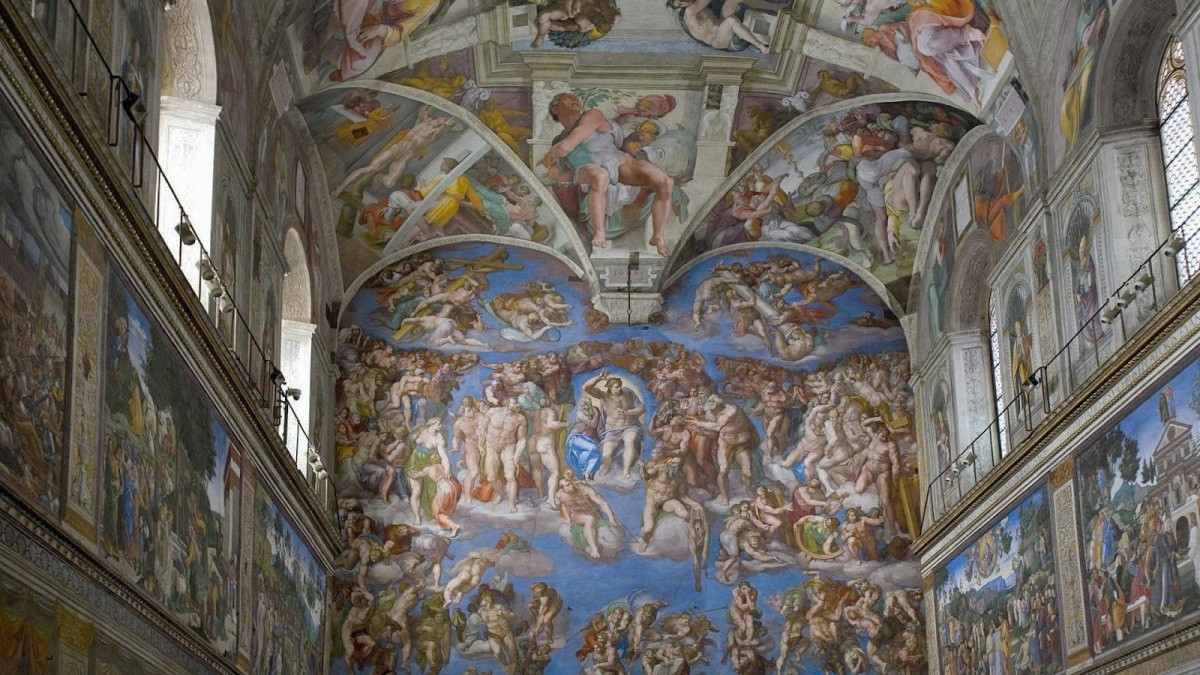
\includegraphics[width=0.7\textwidth]{imagenes/2/capilla-sixtina.jpg}
        \caption{Miguel Ángel Buonarroti, \textit{Capilla Sixtina}, 1508-1512}
        \label{fig:capilla-sixtina}
    \end{center}
\end{figure}

\subsection{Barroco}

La última etapa renacentista del Manierismo fue revelando lo que ocurriría con las artes a partir del siglo XVII. El Barroco fue la etapa de eclosión de una arquitectura grandilocuente y teatral que cumplió con una doble función: por un lado, la de manifestar el poder de los comitentes de la obra, que utilizaban la arquitectura como auténtica propaganda política; y por otro lado, en la arquitectura religiosa, la de adoctrinar a unos fieles fácilmente impresionables. Las iglesias se recubrieron de pinturas murales, que ocuparon también las bóvedas a modo de rompimientos celestes, y de ciclos escultóricos que representaron la vida de Cristo y de los Santos, sirviendo sus figuras como modelos de vida. La pintura encontró en esta época su momento más destacado hasta la fecha en cuanto a técnica y revaloración social. Pintores de la talla de Caravaggio en Italia o de Velázquez en España introdujeron una nueva manera de plasmar el mundo a través de unas composiciones cada vez más complejas y la técnica del claroscuro.

\subsection{Siglo XIX}

En sus últimos momentos, el Barroco adquiere una profusión decorativa y un nivel de recargamiento inusitados en la Historia de los estilos. Los arquitectos del siglo XIX vinieron a romper con esta grandilocuencia y condujeron a la arquitectura hacia el academicismo y la mesura. No obstante, no se puede hablar de homogeneidad estilística en toda la centuria. La arquitectura, si se caracterizó por algo, fue por el eclecticismo y la recuperación de tendencias pasadas a través de los historicismos. Así, volvemos a encontrar cresterías en el Neogótico, grandes órdenes arquitectónicos en el Neoclásico o rasgos de inspiración hispanomusulmana en el Neomudéjar, entre otros.

Lo mismo ocurrió con la pintura. La mayor libertad en el sistema artístico permitió que los artistas elaboraran unos estilos cada vez más personales, dando lugar a unas producciones muy dispares. Románticos, realistas, impresionistas, simbolistas, y un largo etcétera hicieron de este siglo uno de los más prolíficos y originales hasta el momento.

\begin{figure}[!h]
    \begin{center}
        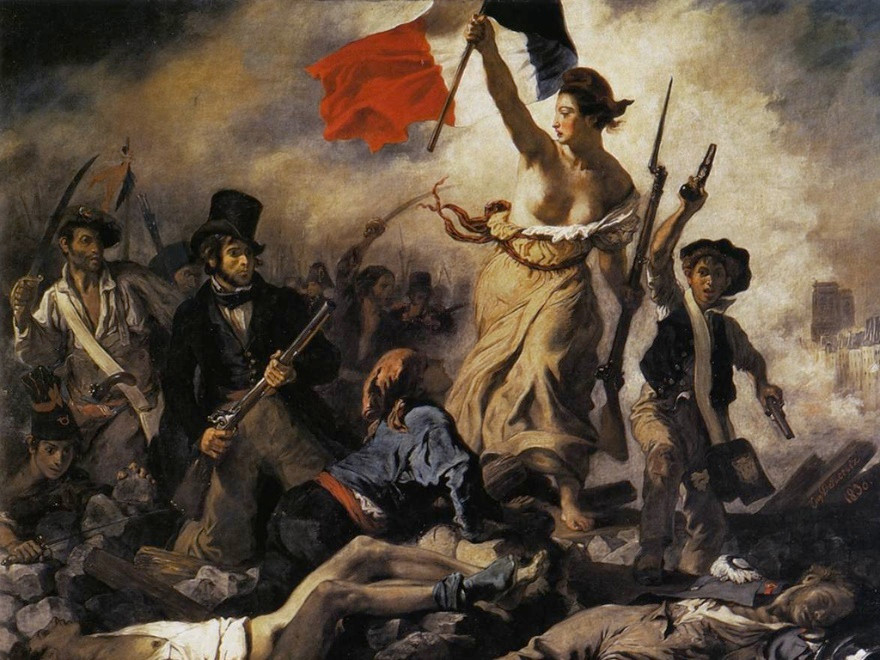
\includegraphics[width=0.7\textwidth]{imagenes/2/libertad-guiando.jpg}
        \caption{Delacroix, \textit{La libertad guiando al pueblo}, 1830}
        \label{fig:libertdad-guiando-pueblo}
    \end{center}
\end{figure}

\subsection{Siglo XX}

Los movimientos de vanguardia vinieron a transformar profundamente y sin retorno a la totalidad de las artes. La arquitectura dejó atrás las formas tradicionales de los historicismos y empezó a hacer uso de los nuevos materiales y tecnologías, además de aumentar su preocupación por el entorno circundante. Aunque tampoco podemos hablar de homogeneidad total, el racionalismo fue la tendencia predominante y la que más impronta dejó en el panorama arquitectónico del siglo XX. Autores como Le Corbusier y Wright levantaron unos edificios ante todo funcionales sirviéndose de líneas puras, formas geométricas y módulos regulares.

En plástica, las vanguardias se manifestaron en lo que ha pasado a la historia como \textit{ismos}. Incontables tendencias de gran originalidad y complejidad teórica coincidieron temporal y espacialmente. Una de las primeras fue el Fauvismo, y su técnica, la más temperamental hasta la fecha, dando todo el protagonismo al color usado de manera emotiva; el Expresionismo, subjetivo y visceral; el Cubismo, rompedor en su visión simultánea de la realidad; el Futurismo y su violencia teórica y expresiva, acorde con el momento histórico del que es fruto; el Surrealismo y su dimensión onírica; y la abstracción en todas sus vertientes, entre otros.

Todas estas corrientes abrieron el camino a un arte definitivamente plural e inclasificable, además de nuevos géneros como la instalación, la \textit{performance} y el arte sonoro, y un sistema de mercado que se ha convertido en el verdadero dueño del devenir artístico.

\subsection{Aplicaciones}

La Historia del Arte ha sido una rama de estudio que siempre ha generado mucho interés, y prueba de ello son las innumerables aplicaciones destinadas a mostrarla de manera didáctica y divulgativa.

En lo que refiere a páginas web existen muchos portales, como \textit{SmartHistory}\footnote{\url{https://smarthistory.org/}} o \textit{The Museum With No Frontiers}\footnote{\url{http://www.museumwnf.org/}}, que proporcionan de manera gratuita y desinteresada toda clase de contenidos y recursos de temática artística.

También, y motivado por la amplia disponibilidad de dispositivos móviles entre la población actualmente, existen diversidad de aplicaciones móvil con este mismo fin, como son \textit{Google Arts \& Culture}\footnote{\url{https://play.google.com/store/apps/details?id=com.google.android.apps.cultural}} que permite a sus usuarios visitar virutalmente exposiciones de arte, o \textit{DailyArt}\footnote{\url{https://play.google.com/store/apps/details?id=com.moiseum.dailyart2}} para Android, que cada día ofrece la imagen y descripción de una obra de arte, ambas también gratuitas.

Y por último, en lo que refiere a videojuegos, se han desarrollado multitud de ellos con temática artística y de museos. Un ejemplo de ello, y en lo que refiere a aventuras gráficas, en 1992 fue lanzado \textit{The Dagger of Amon Ra}, en el que el jugador debe resolver un asesinato en un museo egipcio. Hay muchos más y de muchos otros géneros, como \textit{Discover Babylon}, \textit{Time Explorer} o \textit{Versailles – A game of intrigue at the Court of Louis XIV}.

\section{Realidad Virtual}

Podríamos decir que, en resumen, la Realidad Virtual es una herramienta capaz de crear entornos creíbles, inmersivo e incluso multisensoriales para sus usuarios, de manera que sientan que están en un sitio en el que realmente no están; es decir, se encuentran en un \textbf{mundo virtual}.

Antes de empezar a hablar de la Realidad Virtual, sin embargo, es importante diferenciar los conceptos Realidad Virtual, Realidad Aumentada y Realidad Mixta. Mientras que el primero intenta sumergir por completo al usuario en un mundo virtual, la \textbf{Realidad Aumentada} propone complementar el entorno real superponiendo sobre él objetos digitales. Por último, la \textbf{Realidad Mixta}  une ambos conceptos para permitir interactuar con objetos reales dentro de un mundo virtual, estar completamente inmerso en un mundo virtual o reproducir elementos virtuales en un entorno real.

Los orígenes del concepto de Realidad Virtual no están claros del todo ya que, aplicando la definición anterior, en la época del Renacimiento y con el desarrollo de las técnicas artísticas de perspectiva los propios pintores eran capaces de crear mundos realistas que no existían \cite{schn-17}. 

Sin embargo, las primeras referencias más modernas a este concepto vienen de la mano de un autor de cine. En los años 50 el cineasta \textbf{Morton Heilig} propuso un \textit{experiencia de teatro} con la que poder engañar a los sentidos del  público para transportarles a otro momento y lugar. Pocos años después, en 1962, construyó un prototipo llamado \textbf{Sensorama}, un artilugio capaz de despertar varios de los sentidos de sus usuarios (figura \ref{fig:sensorama}). Este artilugio era capaz de generar en sus usuarios la experiencia de montar en moto en las calles de Brooklin sintiendo el viento en la cara, la vibración del asiento de la motocicleta, una vista tridimensional y los olores de la ciudad. Sin embargo, debido a lo caro que era, no pudo continuarse con su producción \cite{brock-16}.

\vspace{0.2cm}

\begin{figure}[!h]
    \begin{center}
        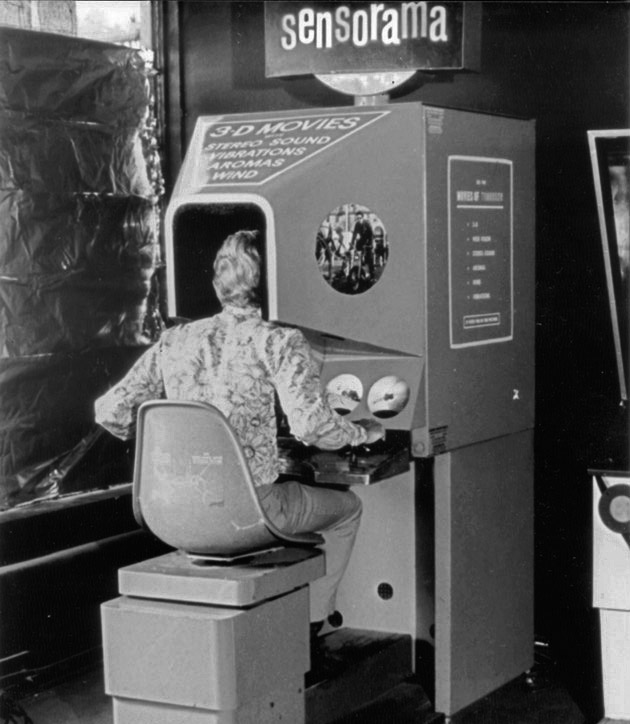
\includegraphics[width=0.5\textwidth]{imagenes/2/sensorama.jpg}
        \caption{Máquina \textit{Sensorama}, \url{www.engadget.com}}
        \label{fig:sensorama}
    \end{center}
\end{figure}

Tres años después, en 1965, el ingeniero \textbf{Ivan Sutherland} escribió el artículo \textit{A head-mounted three dimensional display} \cite{suth-65}, o por sus siglas \acs{HMD}, en el que describe a las imágenes bidimensionales como poco inmersivas y propone un casco con una pequeña pantalla en cada ojo que hacen uso de la \textbf{visión estereoscópica} del ser humano.

Tres años después de la publicación de este artículo, en 1968, Iván Sutherland y su estudiante Bob Sproull desarrollaron el que se considera primer dispositivo para aplicaciones inmersivas. Dado su abultado tamaño, como puede verse en la figura \ref{fig:damocles}, finalmente se le acabó llamando \textbf{\textit{Sword of Damocles}}. Además, este dispositivo contaba con rastreador posicional del casco, por lo que la posición de las imágenes que se visualizaban a través de él correspondía con con su posicionamiento virtual. Pese a todo, y como aún no se disponía de la suficiente tecnología, los gráficos eran muy básicos \cite{lop-18}.

\vspace{0.1cm}

\begin{figure}[!h]
    \begin{center}
        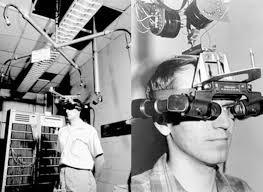
\includegraphics[width=0.7\textwidth]{imagenes/2/damocles.jpg}
        \caption{\textit{Sword of Damocles}, \url{www.dsource.in}}
        \label{fig:damocles}
    \end{center}
\end{figure}

A lo largo de los años setenta, se siguieron desarrollando varios prototipos como \textit{Grope}, de la Universidad de Carolina del Norte, o \textit{Videoplace}, que detectaba mediante cámaras las siluetas de las sombras de los usuarios y las proyectaba sobre una pantalla, lo que les permitía interactuar con ellas \cite{gerv-99}.

Los años 80 fueron muy prolíficos para los simuladores de Realidad Virtual y, paralelamente, comenzaron las primeras discusiones entre diversos filósofos tecnológicos, como Jaron Lanier, Myron Krueger o Ted Nelson, por la búsqueda del término que definiera una tecnología aún en proceso de nacer \cite{lop-18}.

En 1982, Thomas Furnes desarrolló el simulador más avanzado del momento, el \textit{Visually Coupled Airborne Systems Simulator}, o VCASS, que estaba contenido en su totalidad dentro del casco \cite{cade-08}. Aún así seguía siendo bastante voluminoso, como puede verse en la figura \ref{fig:VCASS} 

\begin{figure}[H]
    \begin{center}
        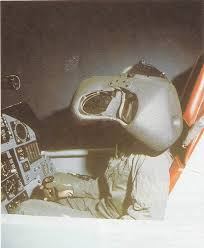
\includegraphics[width=0.45\textwidth]{imagenes/2/VCASS.jpg}
        \caption{\textit{VCASS}, \url{voicesofvr.com}}
        \label{fig:VCASS}
    \end{center}
\end{figure}

Finalmente, el término \textit{Realidad Virtual} fue acuñado por Jaron Lanier, fundador de una de la empresas VPL Research, una de las primeras en comercializar estos sistemas a gran escala \cite{fer-02}. Lanier proponía unos dispositivos que, acoplados en nuestro cuerpo, fueran capaz de hacernos percibir a través de los sentidos sensaciones realistas de un mundo diferente al nuestro, de tal manera que cuanto más avanzados sean estos dispositivos más realistas serán las sensaciones y más difícil será diferenciar entre este mundo y el real \cite{lop-18}.

Y poco a poco, principalmente movido por la creciente industria del videojuego y sus múltiples usos potenciales, estas tecnologías han seguido desarrollándose. Una de las primeras aplicaciones comerciales en los videojuegos fue la \textit{Virtual Boy} de Nintendo. Fue lanzada al mercado en 1995 y contaba con dos pequeñas pantallas monocromáticas que reproducían juegos. Este dispositivo puede verse en la figura \ref{fig:virtual-boy}.

\begin{figure}[H]
    \begin{center}
        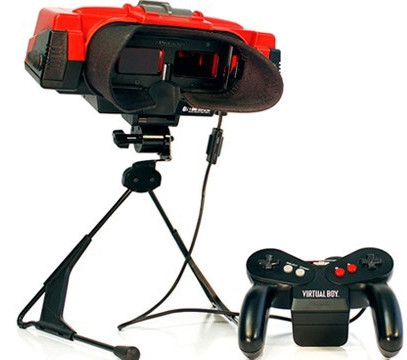
\includegraphics[width=0.45\textwidth]{imagenes/2/virtual-boy.jpg}
        \caption{\textit{Virtual Boy}, \url{codigoespagueti.com}}
        \label{fig:virtual-boy}
    \end{center}
\end{figure}

Aunque esta consola fue un fracaso (apenas se vendieron 770.000 unidades en todo el mundo\footnote{\url{http://www.gamepro.com/gamepro/domestic/games/features/111823.shtml}, 2007}) demostró que se podían desarrollar dispositivos similares.

Y con esto llegamos a la actualidad, donde poco a poco, y principalmente por el abaratamiento de esta tecnología, el mercado de dispositivos de Realidad Virtual está creciendo y cada vez hay más dispositivos al alcance de los usuarios.

\subsection{Dispositivos}

Actualmente, los principales dispositivos que permiten jugar en \acs{VR} destinados a usuarios normales y que, por tanto, son en los que se ha centrado este \acs{TFM}, son los siguientes.

\subsubsection{Oculus Rift} 

En el año 2012, Palmer Lucky fundó la compañía Oculus VR con la idea de crear un dispositivo destinado a jugar en \acs{VR} y con un precio viable para los jugadores casuales. A finales de ese mismo año, y con ayuda de John Carmack (programador en juegos como Doom, Quake o Wolfenstein), mostró el primer prototipo del dispositivo y fue un éxito, por lo que lanzó una campaña en Kickstarter que superó con creces el dinero necesario, consiguiendo caso 2 millones y medio de dólares\footnote{\url{https://www.kickstarter.com/projects/1523379957/oculus-rift-step-into-the-game}} y que puede verse en la figura \ref{fig:oculus}.
    
\begin{figure}[!h]
\begin{center}
    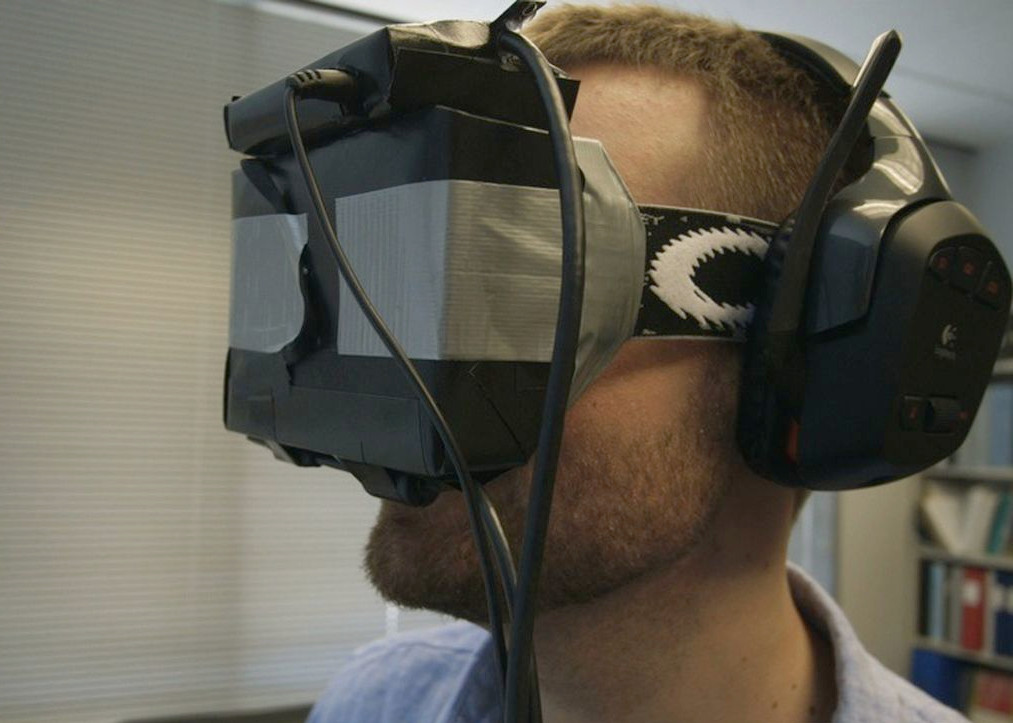
\includegraphics[width=0.5\textwidth]{imagenes/2/oculus-prototipo.jpg}
    \caption{Prototipo del \textit{Oculus Rift}, \url{www.theverge.com}}
    \label{fig:oculus}
\end{center}
\end{figure}

Año tras año fue mejorando sus prototipos hasta que en marzo de 2014 Facebook compró esta compañía por un total de 2,300 millones de dólares. Finalmente, en mayo de 2015, se anunció la versión finalizada de las gafas lista para su comercialización. Actualmente pueden comprarse por unos 240\euro.

\subsubsection{HTC Vive} 

Vive son unas gafas de realidad virtual co-fabricadas por HTC y Valve. En 2014 se mostraron los primeros prototipos de un sistema de realidad virtual producido por la empresa Valve, pero no fue hasta marzo de 2015 cuando HTC reveló oficialmente las Vive. Antes de la versión para consumidores se fabricaron las Vive PRE, que fueron gratuitas para algunos desarrolladores de videojuegos con el fin de promover sus aplicaciones. 

\begin{figure}[!h]
\begin{center}
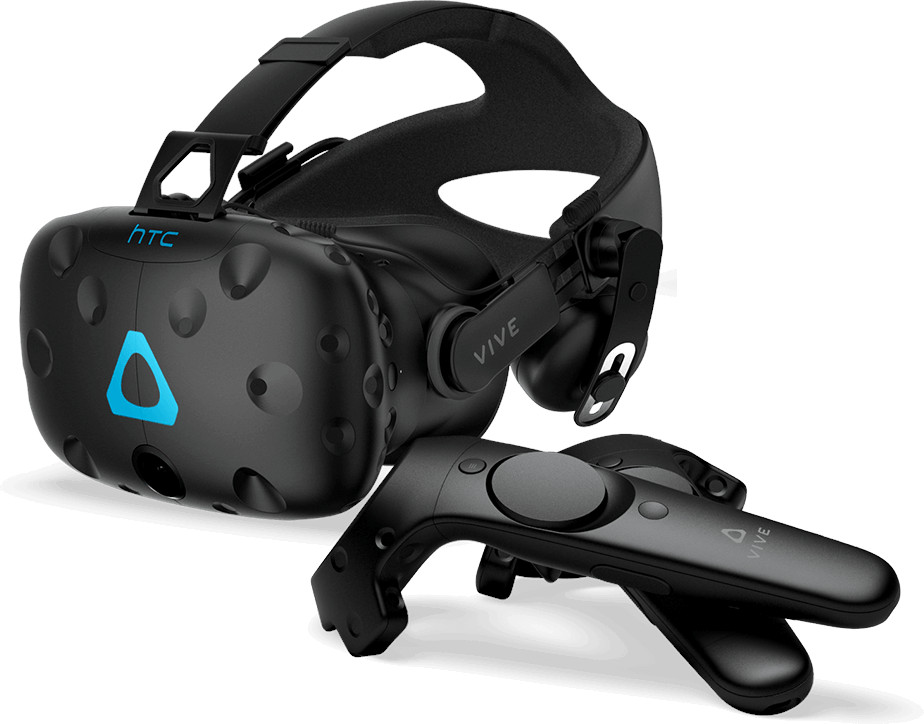
\includegraphics[width=0.5\textwidth]{imagenes/2/htc-vive.jpg}
\caption{HTC Vive}
\label{fig:htc-vive}
\end{center}
\end{figure}

A principios de 2016 se anunció su lanzamiento con un precio de salida de 900\euro, aunque actualmente pueden adquirirse por la mitad, unos 450\euro.

\subsubsection{PlayStation VR} 

Este headset no es la primera propuesta de PlayStation de \acs{VR}. Su primer intento comercial, \textit{Glasstron}, se lanzó en 1997 para el juego \textit{MechWarrior 2}. Estas gafas permitían a jugadores adoptar una perspectiva visual desde dentro de la cabina de la nave, como si la controlaran.

\vspace{0.1cm}

\begin{figure}[!h]
\begin{center}
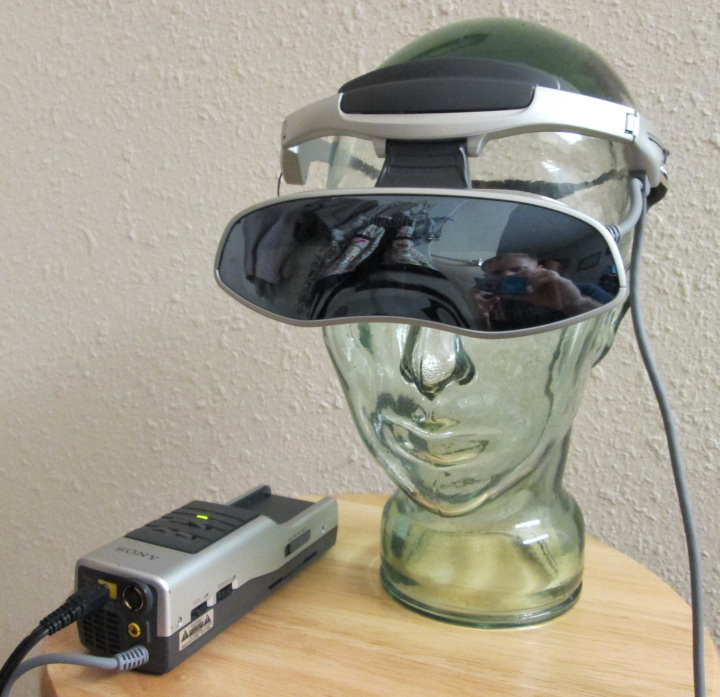
\includegraphics[width=0.5\textwidth]{imagenes/2/glasstron.jpg}
\caption{Gafas \textit{Glasstron}, \url{http://www.mellottsvrpage.com}}
\label{fig:glasstron}
\end{center}
\end{figure}

A mediados de 2014, el desarrollador de PlayStation Anton Mikhailov anunció en una conferencia que su equipo había estado trabajando en el Project Morpheus durante 3 años, rediseñando el \textit{PlayStation Move} para adaptarlo a la tecnología \acs{VR}. Al año siguiente este proyecto se bautizó como \textit{PlayStation VR}. Finalmente lanzada al mercado en 2016, actualmente puede comprarse por unos 250\euro, aunque solo funciona con un sistema PlayStation 4.
    
\subsubsection{Lenovo Explorer} 

La compañía Lenovo también ha dado el salto a los headsets \acs{VR} desarrollando uno propio, llamado Explorer. Este dispositivo, lanzado al mercado en octubre de 2017, hace uso del \textit{Microsoft Mixed Reality}, un framework de desarrollo implementado por Microsoft para su headset \acs{AR}, las \textit{Microsoft HoloLens}. Como su nombre sugiere, este framework está pensado para trabajar tanto con tecnologías \acs{VR} como \acs{AR}.
    
A diferencia del resto de headsets, el Explorer tiene dos pequeñas cámaras integrados en la parte delantera, lo que le permite escanear y transmitir la ubicación del usuario, de los mandos y del entorno haciendo uso de la tecnología de rastreo sin balizas de Microsoft, similares a las que se usan para HoloLens. Además incluye dos controladores, como puede verse en la figura \ref{fig:lenovo-explorer}.

\begin{figure}[!h]
\begin{center}
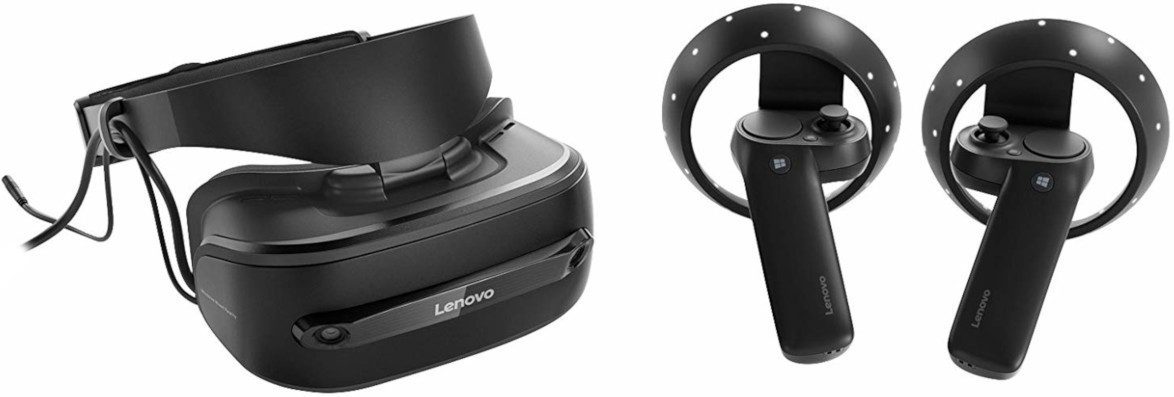
\includegraphics[width=0.8\textwidth]{imagenes/2/lenovo-explorer.jpg}
\caption{Gafas \textit{Lenovo Explorer}}
\label{fig:lenovo-explorer}
\end{center}
\end{figure}

Además, tienen el precio más competitivo de todas, llegando a haber podido ser compradas en la página \url{pccomponentes.com} por 150\euro, como puede verse en la figura \ref{fig:precios-explorer}, aunque actualmente ronde los 200\euro. 

\begin{figure}[!h]
\begin{center}
    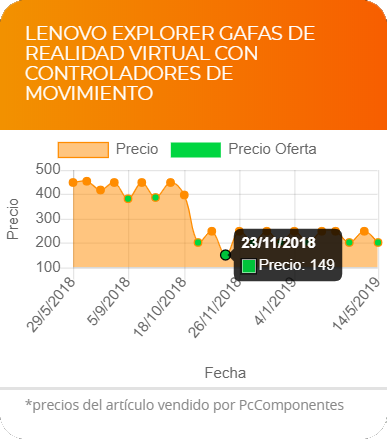
\includegraphics[width=0.4\textwidth]{imagenes/2/precios-explorer.png}
    \caption{Historial de precios de las Lenovo Explorer, \url{pccomponentes.com}}
    \label{fig:precios-explorer}
\end{center}
\end{figure}

Por todo esto se cree que son las más probables para ser adquiridas en los jugadores interesados en esta tecnología, por lo que han sido elegidas para usarse en este proyecto. En el capítulo \ref{chap:tecnologia} se hablará en más profundidad de su tecnología y sus especificaciones técnicas.

\subsubsection{Google Cardboard} 

La opción más económica para comenzar en el mundo de la \acs{VR} son los headsets de cartón. El más famoso es el de Google, que permite usar un teléfono móvil como pantalla para abaratar mucho los costes, de manera que el headset es simplemente una caja de cartón vacía con dos pequeñas lentes para los ojos, como puede verse en la figura \ref{fig:google-cardboard}, y que puede comprarse en Amazon por menos de 10\euro.
    
\begin{figure}[!h]
\begin{center}
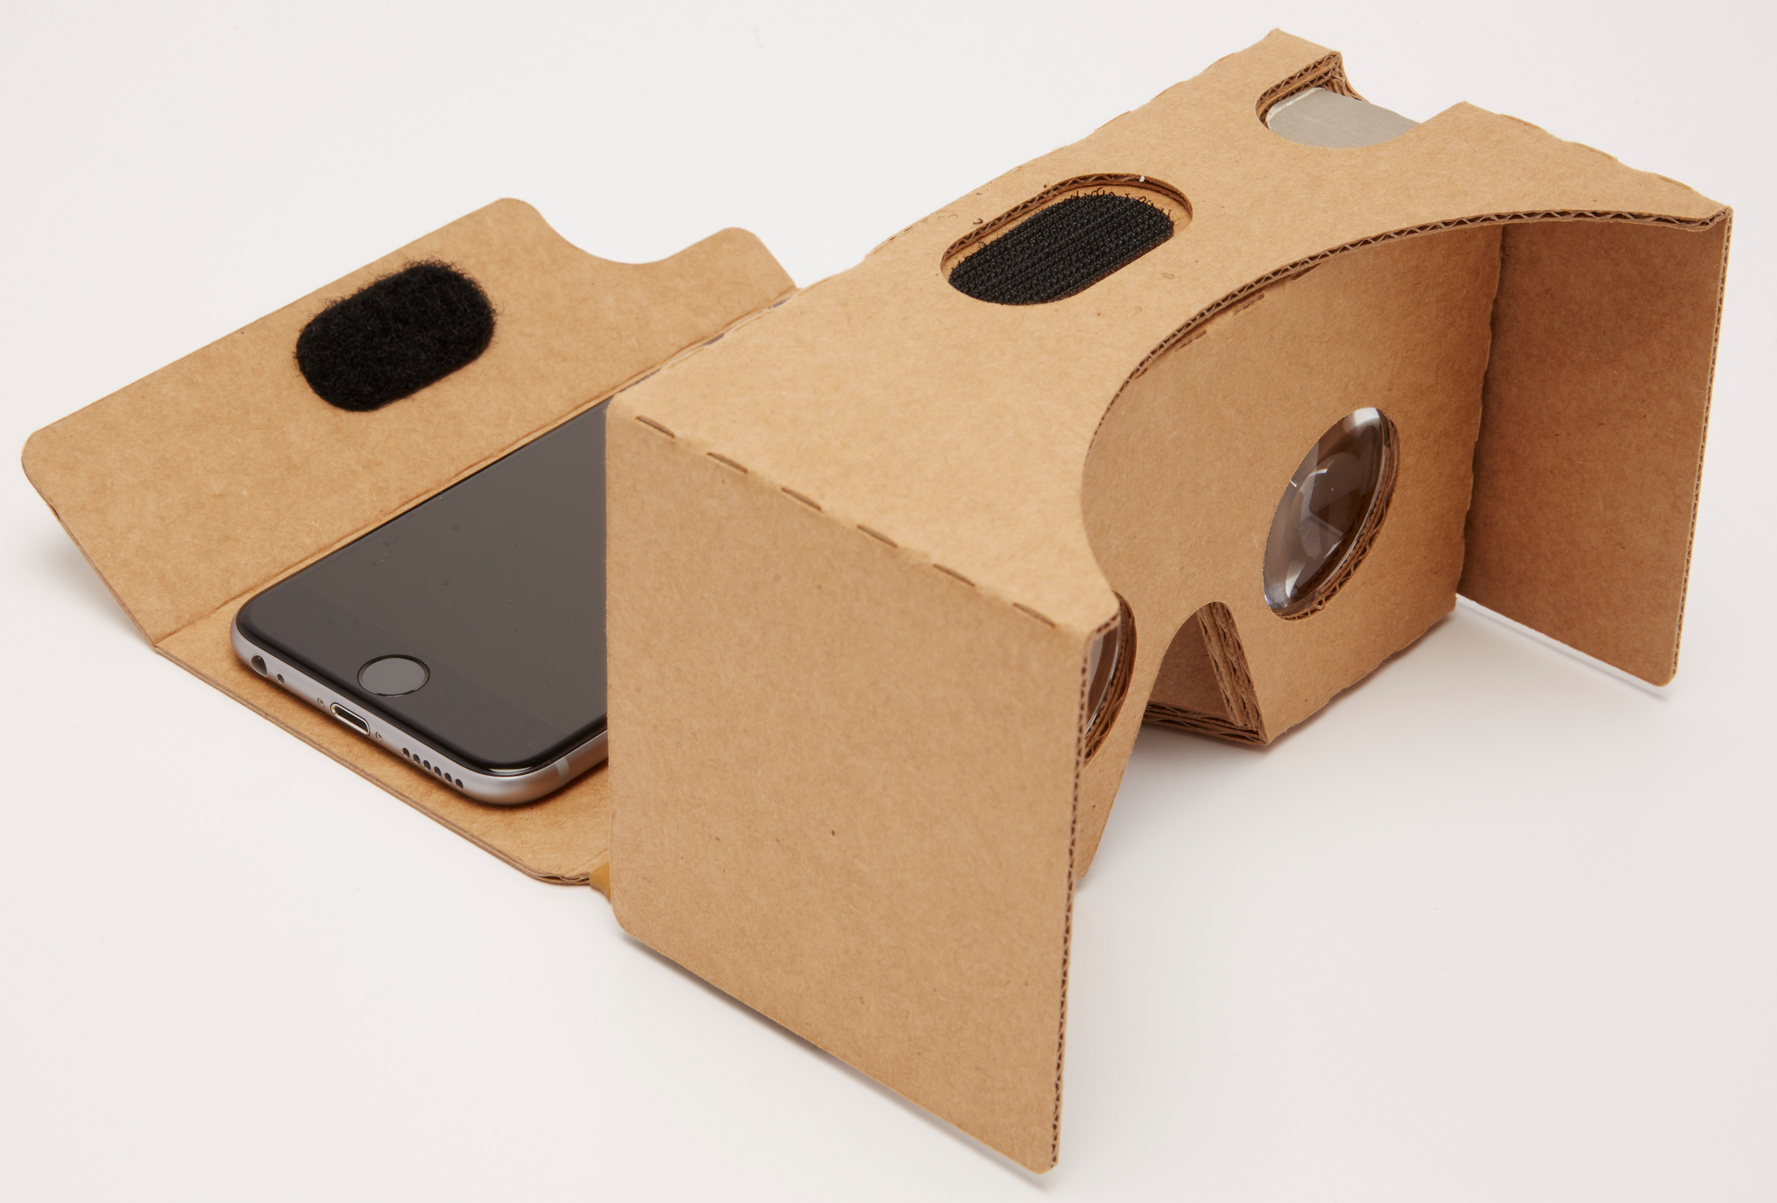
\includegraphics[width=0.5\textwidth]{imagenes/2/cardboard.jpg}
\caption{Google Cardboard abiertas}
\label{fig:google-cardboard}
\end{center}
\end{figure}

El principal problema es que los móviles, al no ser dispositivos especialmente potentes, no permiten el renderizado de escenarios complejos, por lo que no consiguen una sensación de inmersión muy buena.

\subsubsection{Index VR}

Anunciado por Valve en mayo de este año y aún no disponible para comprar, Index VR\footnote{\url{https://www.valvesoftware.com/es/index}} es el último headset incluido en la lista. Es un dispositivo para jugar en \acs{VR} compuesto por un headset, dos controladores y dos estaciones de posicionamiento (figura \ref{fig:index-vr}) que, según la propia Valve, permitirán un \textit{tracking} mucho más preciso de la posición y los movimientos de los jugadores, que podrán moverse libremente en un área de 10x10 metros.

\begin{figure}[!h]
\begin{center}
    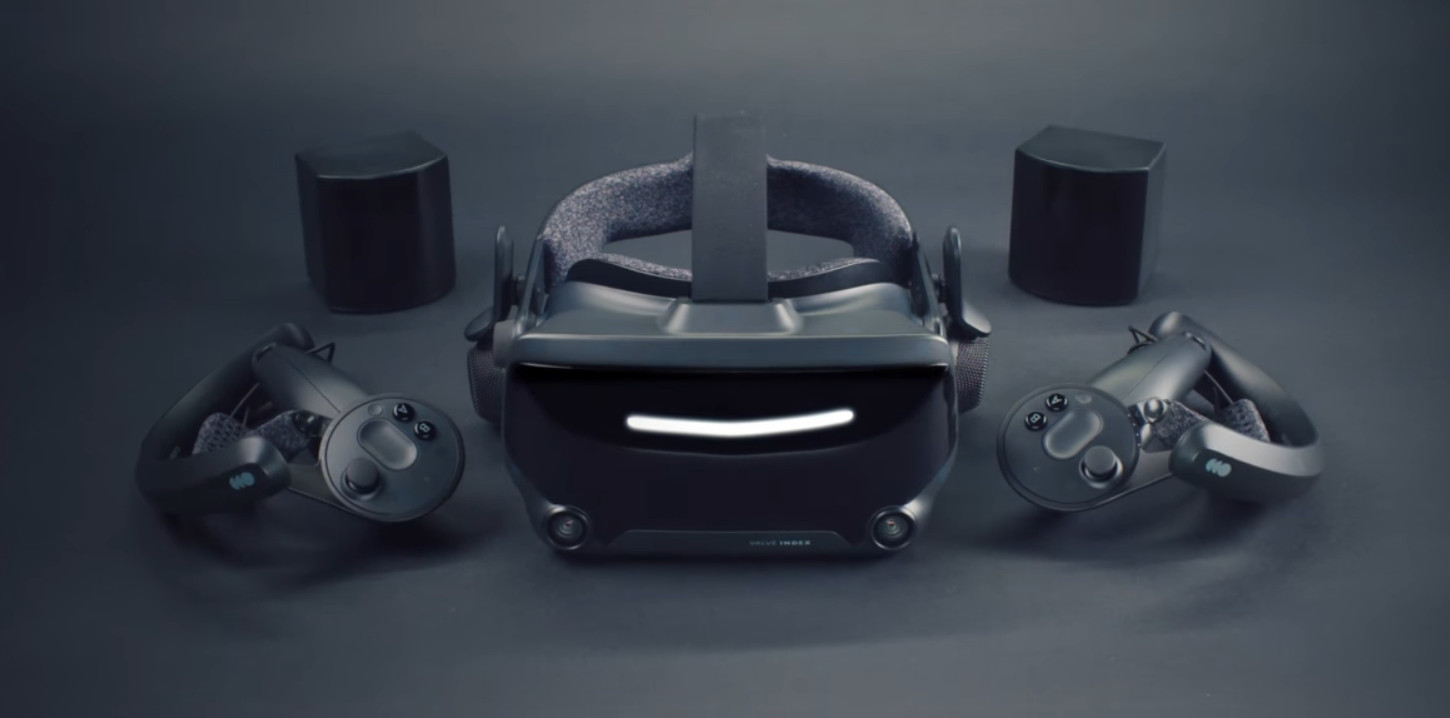
\includegraphics[width=0.85\textwidth]{imagenes/2/indexvr.jpg}
    \caption{\textit{IndexVR} de Valve}
    \label{fig:index-vr}
\end{center}
\end{figure}

Por otro lado, es de lejos el dispositivo destinado al público general más caro del mercado, estando disponible para reserva el pack con los tres periféricos anteriormente presentados por 1080\euro.

\subsection{Librerías de desarrollo}

Como la Realidad Virtual es una tecnología relativamente nueva que aún no se ha abaratado todo lo que puede, no ha conseguido llegar a los hogares de la mayoría de sus potenciales usuarios. Por tanto, como la demanda es muy baja, la oferta de aplicaciones también lo es y, en consecuencia, hay muy pocas empresas que hayan invertido en desarrollar frameworks y librerías de desarrollo para aplicaciones que hagan uso de la Realidad Virtual.

Aún así, han aparecido algunas librerías desarrollados por empresas con la mayor cuota de mercado y que pueden permitirse innovar, como Steam, y otras que se han centrado en esta tecnología y lo necesitaban, como Oculus. A continuación se presentan las más importantes.

\subsubsection{VRTK}

\acl{VRTK}\footnote{\url{https://vrtoolkit.readme.io}} es un framework de desarrollo multi-librería desarrollado en solitario bajo licencia \acs{MIT} por \textit{TheStoneFox}\footnote{\url{https://github.com/thestonefox}}, o Harvey Ball, un hombre residente en Birmingham, Reino Unido. Este framework solo está disponible para el \acs{IDE} Unity3D y permite desarrollar paralelamente para distintas librerías a través de una interfaz común; es decir, podemos desarrollar para SteamVR y Oculus a la vez usando la interfaz de \acs{VRTK}.

Pero el desarrollo de esta librería no ha sido fácil para \textit{TheStoneFox}; todo empezó en abril de 2016 cuando, sin apenas experiencia en desarrollo de videojuegos, comenzó un proyecto con Unity3D y SteamVR y se dio cuenta de lo confuso y poco documentado que estaba todo, por lo que decidió desarrollar su propio \acs{SDK} o, en sus propias palabras\footnote{\url{https://uploadvr.com/vrtk-stone-fox-unity-tool/}},

\begin{displayquote}
\textit{I wanted to build something for it as I was new to game dev. I’d been using Unity for about a month just as a hobby, I tried to use the SteamVR Unity plugin and found it confusing, realized a lot of people found it confusing and started VRTK as a way to help people get into developing for VR."}
\end{displayquote}

Y poco a poco fue avanzando en su proyecto y ganando la atención de los desarrolladores hasta que decidió abrirse una cuenta de Patreon\footnote{\url{https://www.patreon.com/vrtk}}, donde llegó a ingresar 2000\$ al mes, y lo que comenzó como un pasatiempo a tiempo parcial se conviritó en su único proyecto. Además, comenzó a realizar conferencias por todo el mundo gracias a las que fue ganando popularidad, como la \textit{Unite Europe 2017}, cuya ponencia puede verse en YouTube\footnote{\url{https://youtu.be/AbIiBrg8yT4}}.

Pero a finales de 2017, entre el nulo apoyo que recibía de la comunidad, que hacía que él fuera literalmente el único desarrollador del proyecto (como puede verse en la figura \ref{fig:stonefox-twitter}), y que no quería que la cuenta de Patreon diera la impresión de que el proyecto era solvente, porque no lo era, decidió cerrar esta cuenta y dar por finalizado el proyecto. Aún así, aunque dijo que no añadiría funcionalidad nueva, se comprometió a seguir manteniéndolo durante algún tiempo, principalmente arreglando bugs\footnote{\url{https://skarredghost.com/2017/12/28/vrtk-shutting-will-make-vr-development-unity-easier-now/}}.

\begin{figure}[!h]
\begin{center}

\includegraphics[width=0.8\textwidth]{imagenes/2/stonefox-twitter.png}
\caption{\textit{TheStoneFox} en Twitter sobre los motivos del cierre de \acs{VRTK}}
\label{fig:stonefox-twitter}
\end{center}
\end{figure}

Por suerte, cuatro meses después y gracias a una donación por parte de Oculus, el proyecto volvió a la vida. El propio \textit{TheStoneFox} aclaraba en Twitter que no era ningún tipo de compra, ya que \acs{VRTK} seguiría siendo gratuito y mantendría la misma filosofía que antes de cerrarse\footnote{\url{https://skarredghost.com/2018/04/30/vrtk-announces-version-4-thanks-to-an-oculus-grant/}}.

A día de hoy la página de Patreon vuelve a estar abierta, aunque apenas ingresa un tercio de la cantidad de antes de dar por finalizado el proyecto.

Actualmente existen varios proyectos comercializados desarrollados gracias a este framework, como \textit{Deism}, \textit{One of the last} u \textit{Oddescape}. Uno de los más famosos es \textit{quiVr}\footnote{\url{http://quivr.net/}}, un \textit{tower defense} en el que el jugador encarna a un arquero que debe acabar con todas las oleadas de enemigos que aparecen antes de que lleguen a su base.

\textit{TheStoneFox} también realiza pequeños vídeos enseñando todos los juegos que utilizan su framework con el fin de darles publicidad y de mostrar la potencia que tiene. Todos estos vídeos pueden verse en una lista de reproducción\footnote{\url{http://yt.vu/p/PLTiD-q2AfVNIrAN5w0WK6hOyjy6zL1tWv}} en la que los añade. 

\subsubsection{SteamVR}

Steam es una plataforma de distribución digital de videojuegos cuya dueña es Valve. Steam lanzó en 2014 una nueva iniciativa para adaptar la Realidad Virtual a los juegos digitales, llamada SteamVR\footnote{\url{https://steamcommunity.com/steamvr}}, que permite el desarrollo y uso de juegos de realidad virtual a partir de su plataforma, es decir, solo los juegos distribuidos en Steam podrán acceder a estas librerías.

A principios de  2014, Valve inició un proyecto para \acs{VR} para su plataforma. En junio de 2014 se mostraron los primeros avances pero no fue hasta la Mobile World Congress de 2015 cuando se anunció públicamente. El primer dispositivo que usó esta tecnología fue el HTC Vive, el headset \acs{VR} de HTC.

Actualmente la plataforma cuenta con más de 1200 experiencias \acs{VR} con todo tipo de juegos y simuladores. Además, desde 2017 tienen en fases de desarrollo la incorporación de la Realidad Aumentada en colaboración con Microsoft\footnote{\url{https://generacionxbox.com/microsoft-steamvr-realidad-aumentada/}}.

\subsubsection{Windows Mixed Reality}

Windows Mixed Reality, anteriormente Windows Holographic, es una plataforma de \acs{MR} desarrollada por Microsoft e incluida de manera nativa en Windows 10 desde principios de 2018.

El principal dispositivo para este framework son las Microsoft HoloLens, un headset que en realidad es un ordenador inalámbrico autónomo corriendo Windows 10. Utiliza sensores avanzados, dos pantallas estereoscópicas de alta definición y sonido espacial que le permiten ejecutar aplicaciones de realidad aumentada.

Las HoloLens estuvieron desarrollándose durante casi cinco años antes de su lanzamiento público en 2015, aunque inicialmente fue concebido no como un headset independiente sino como una tecnología para la cámara Kinect\footnote{\url{https://www.wired.com/2015/01/microsoft-hands-on/}}.

Inicialmente, las HoloLenses únicamente estaban disponibles en Norteamérica, pero gracias a la positiva respuesta que han recibido de parte de sus usuarios llegarán próximamente a Europa.

Además, con el fin de atraer a más usuarios, Microsoft ha lanzado \textbf{Windows Mixed Reality for SteamVR}, un wrapper que permite jugar a juegos desarrollados con la librería SteamVR con un headset que implemente su tecnología. Es necesario descargar este software desde Steam como si fuera un juego.

\subsubsection{Oculus SDK}

El framework de desarrollo para Oculus, también llamado Oculus SDK\footnote{\url{https://developer.oculus.com/downloads/}}, es un conjunto de librerías desarrolladas por Oculus para su headset \acs{VR}, Oculus Rift.

Este \acs{SDK} está disponible para los IDEs Unity3D y Unreal Engine, además de poder descargarse para trabajar directamente en Windows.
    

\subsection{Aplicaciones}

Los usos de la tecnología \acs{VR} son casi tan variados como los colectivos la utilizan. En esta sección se presentan las principales aplicaciones de la \acs{VR}.

\subsubsection{Simulación}

Una de las aplicaciones más potentes de la \acs{VR} es la simulación. Por su componente inmersivo, la \acs{VR} es perfecta para este tipo de aplicaciones, ya que permite a sus usuarios sentir que están en un entorno diferente sin los peligros que pueda conllevar.

Dentro de la simulación, uno de los campos de aplicación más importantes es el militar, donde poder entrenar a personas para situaciones de riesgo sin poner en peligro sus vidas es de vital importancia.

Un ejemplo de esto es el Departamento de Defensa de los Estados Unidos de América, que ha desarrollado el \textit{Weapons Augmented Reality Scoring System}, o WARSS, un entorno en el que los soldados pueden practicar situaciones y tácticas a las que podrían enfrentarse un día usando tecnologías \acs{VR} y \acs{MR}, concretamente con dispositivo HoloLens de Microsoft, como puede verse en la figura \ref{fig:warss}.

\begin{figure}[!h]
\begin{center}
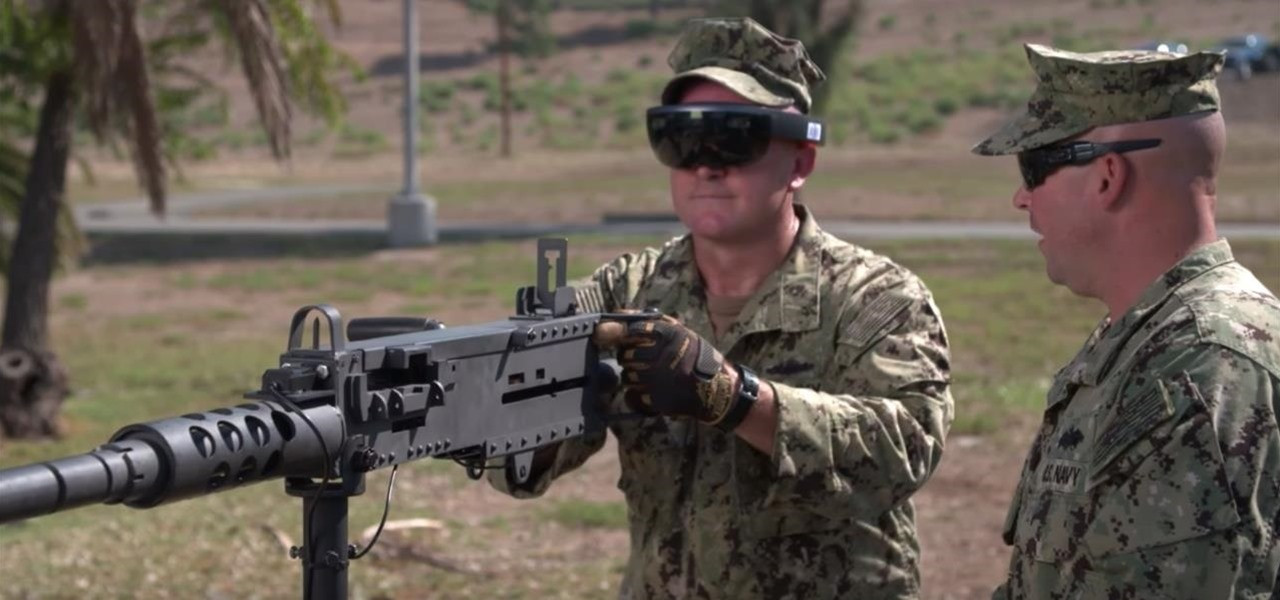
\includegraphics[width=0.8\textwidth]{imagenes/2/WARSS.jpg}
\caption{Soldados del ejército americano haciendo uso de la tecnología WARSS, \url{https://hololens.reality.news}}
\label{fig:warss}
\end{center}
\end{figure}

Otro de los campos en los que triunfa esta tecnología por los mismos motivos es en la la medicina, donde es imprescindible que los médicos sepan cómo manejar situaciones delicadas para la vida de los pacientes antes de tener que enfrentarse a ellas por primera vez ya que, gracias a la ayuda de programadores y modeladores 3D, se puede reproducir con exactitud la anatomía de los pacientes y practicar crujías antes incluso de llevarlas a cabo, reduciendo los costes de utilización de cadáveres para pruebas y permitiendo repetir la operación cuantas veces fuera necesario.

En figura \ref{fig:medico} puede verse a un cirujano con el headset \acs{VR} Oculus Rift haciendo uso de esta tecnología.

\begin{figure}[!h]
\begin{center}
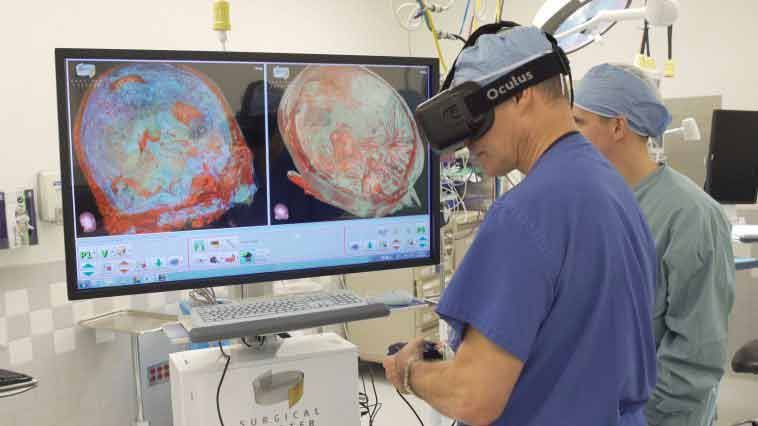
\includegraphics[width=0.8\textwidth]{imagenes/2/medicina.jpg}
\caption{Médico simulando una operación, \url{http://www.baboonlab.com}}
\label{fig:medico}
\end{center}
\end{figure}
 
\subsubsection{Videojuegos}

Como ya se ha expuesto antes, la industria de los videojuegos es actualmente una de las más lucrativas y, como los propios videojuegos requieren de la inmersión de sus usuarios, ha sido fácil para la \acs{VR} abrirse paso a través de ella.

Actualmente, los juegos en \acs{VR} que más éxito tienen en Steam\footnote{\url{https://store.steampowered.com/vr/}} son aquellos en los que el jugador debe disparar, ya sea con armas, como en el caso de \textit{Pavlov VR} o \textit{Blade and Sorcery}, o con arcos, como en \textit{Elven Assassin}, como puede verse en la figura \ref{fig:elven-assassin}.

\begin{figure}[!h]
\begin{center}
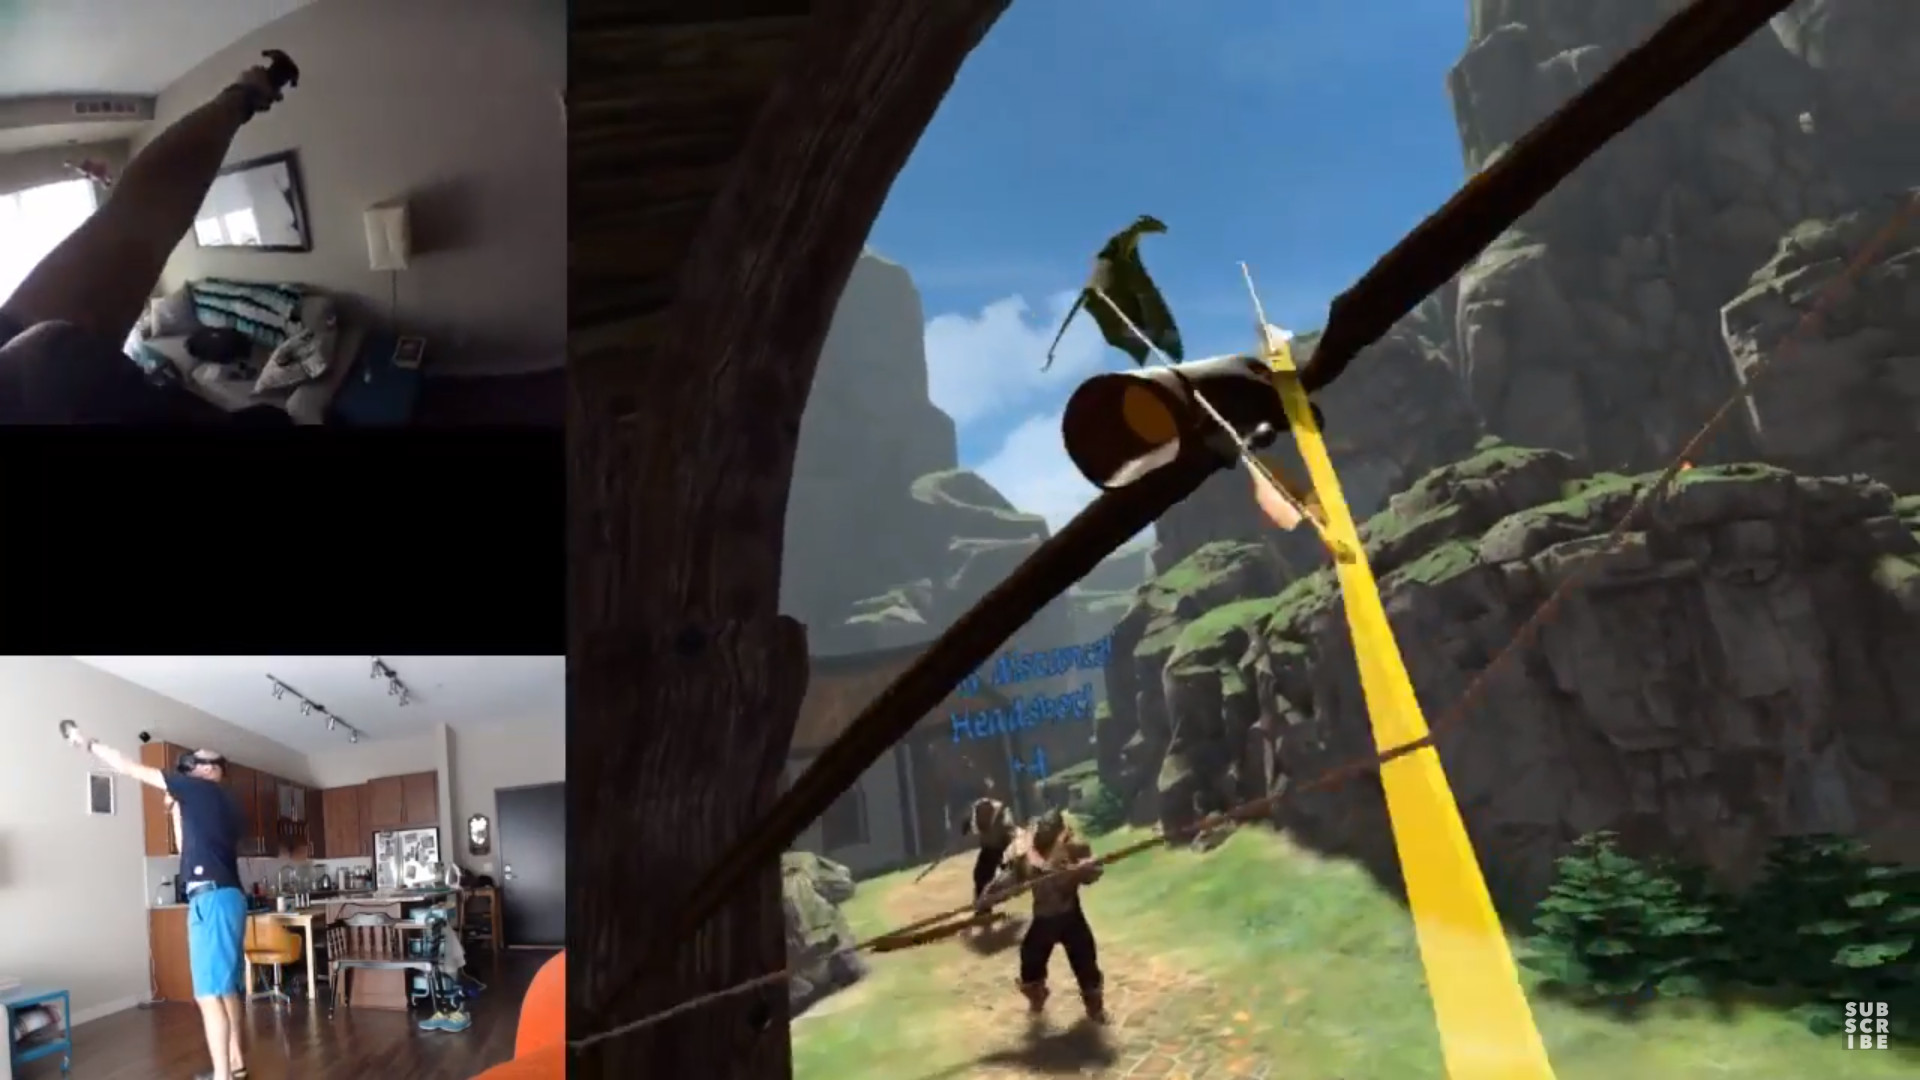
\includegraphics[width=0.7\textwidth]{imagenes/2/elven-assassin.jpg}
\caption{Elven Assassin, \textit{YouTube/BenPlaysVR}}
\label{fig:elven-assassin}
\end{center}
\end{figure}

\subsubsection{Reconstrucción}

Dada la naturaleza inmersiva de la \acs{VR}, es perfecta para, mediante sistemas de modelado tridimensionales, recrear lugares tal y como eran en algún momento de la historia para poder estudiarlos o verlos fácilmente.

Un ejemplo de esto sería las aplicaciones \acs{VR}\footnote{\url{https://uploadvr.com/notre-dame-vr/}} que han surgido a raíz de la cercana trajeada que sufrió la iglesia de Notre-Dame de París en la que un incendio provocó que la mayor parte de su interior se quemara. Estas aplicaciones permiten ver cómo era antes del incendio de un modo mucho más realista e inmersivo que verlo a través de un vídeo.

\section{Diseño 3D}

El diseño 3D es esencial en el desarrollo de \MineRVa, ya que tanto a la hora de diseñar y modelar las salas como implementar sus funcionalidades será necesario basarse en este área.

En esta sección se presentarán y describirán las dos áreas del diseño 3D más importantes para desarrollo de este proyecto.

\subsection{Suites de modelado 3D}

Lo principal a la hora de trabajar con modelos 3D es poder diseñarlos y modelarlos, Para ello, actualmente existen multitud de programas y suites completas a disposición de los usuarios. Los más importantes y con la mayor cuota de mercado son los siguientes. 

\subsubsection{Blender}

Blender\footnote{\url{https://www.blender.org/}} es un programa informático multiplataforma, dedicado especialmente al modelado, iluminación, animación y renderizado de gráficos tridimensionales, además de incluir herramientas para esculpir tridimensionalmente y hasta un motor de juegos propio, el Blender Game Engine. Aunque inicialmente era distribuido de forma gratuita pero sin el código fuente, actualmente es \textit{open source} bajo la licencia GNU General Public License, o GPL, y está disponible para prácticamente todos los sistemas operativos para ordenador.

\begin{figure}[!h]
\begin{center}

\includegraphics[width=0.4\textwidth]{imagenes/2/roosendaal.jpg}
\caption{Tom Roosendaal, imagen obtenida de su cuenta de Twitter}
\label{fig:roosendaal}
\end{center}
\end{figure}

Todo empezó a finales de los años 80 cuando Ton Roosendaal, el futuro fundador de Blender, era el líder de NeoGeo, el mayor estudio de animación de Holanda. Por aquel entonces la herramienta 3D que utilizaban era muy lenta y cara de mantener, por lo que decidieron reescribirla de 0, plantando la semilla de lo que después sería el software de creación que ahora conocemos como Blender\footnote{\url{https://www.blender.org/foundation/history/}}. 

Pero mientras que NeoGeo continuaba trabajando en Blender, Roosendaal pensó que el mundo entero podría beneficiarse de su herramienta, por lo que a finales de los 90 fundó una división de NeoGeo, Not a Number (o NaN a partir de ahora) para distribuir gratuitamente Blender y fomentar su desarrollo y su mercado, ya que la mayoría de los programas comerciales de modelado de la época costaban miles de dólares.

A principios del año 2000, NaN recaudó más de 4,5 millones de euros procedente de sus inversores, y pronto pasó a tener más de 50 empleados trabajando alrededor del mundo intentando mejorar y promocionar Blender, publicando la versión 2.0 unos meses después.

Desafortunadamente, debido a las decepcionantes ventas y al continuo clima de dificultades económicas, los inversores decidieron dar por terminado el desarrollo de Blender. Pero por suerte Roosendaal no permitió que Blender desapareciera, así que en marzo de 2002 fundó la organización no lucrativa Blender Foundation, cuyo primer objetivo fue continuar con el desarrollo como un proyecto de código abierto basado en la comunidad de usuarios.

La compañía tuvo que obtener 100,000\euro \ para poder comprar los derechos del código fuente y los de propiedad intelectual de Blender a su antigua compañía, NaN, que consiguieron ser reunidos por la comunidad en menos de 7 semanas. Finalmente, el 13 de octubre de 2002, Blender fue liberado al mundo bajo los términos de GNU General Public License. 

Actualmente, el desarrollo de Blender sigue gracias a un equipo de voluntarios procedentes de diversas partes del mundo, liderados por Ton Roosendaal, que continúan actualizándolo gracias a las donaciones en su página web, obteniendo actualmente 36,521\euro \ al mes\footnote{\url{https://fund.blender.org/}}. Además, periódicamente realizan cortos en los que muestran la potencia de su herramienta como \textit{Big Buck Bunny}, \textit{Caminandes}, \textit{Sintel} o \textit{Agent 327}.

\begin{figure}[!h]
\vspace{0.5cm}
\begin{center}
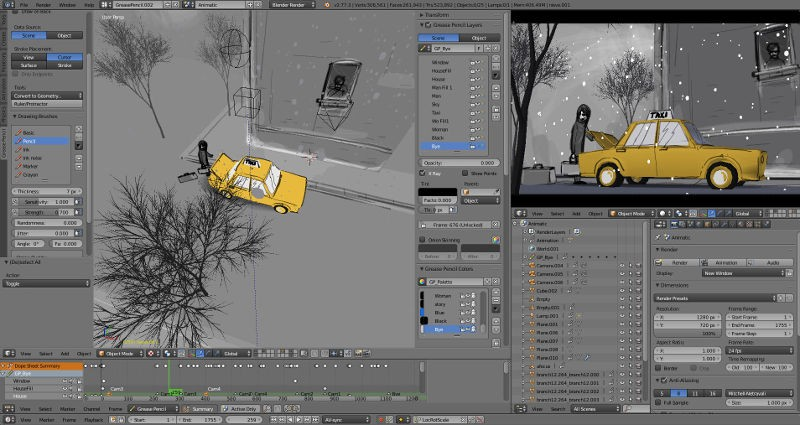
\includegraphics[width=0.9\textwidth]{imagenes/2/blender.jpg}
\caption{Captura de pantalla del entorno de trabajo de Blender}
\label{fig:blender}
\end{center}
\vspace{-0.5cm}
\end{figure}

\subsubsection{Autodesk Maya}

Maya es un programa informático dedicado al desarrollo de gráficos 3D por ordenador, efectos especiales y animación. Además, es el único software de 3D acreditado con un Oscar gracias al enorme impacto que ha tenido en la industria cinematográfica como herramienta de efectos visuales.

Maya surgió tras la fusión de Alias y Wavefront, dos empresas canadienses dedicadas al \acs{CGI} los gráficos generados por ordenador, ya que ambas se utilizaban de manera conjunta prácticamente siempre. Este programa se desarrolló en estrecha colaboración con Disney durante la producción de Dinosaurio a finales de la década de los 1990. Una de los requisitos de Disney era que la interfaz gráfica de usuario pudiera ser fácilmente personalizable, lo que ayudó a que años después Maya se convirtiera en el estándar de la industria gracias a que cada compañía podía cambiar la \acs{GUI} a su gusto.

Autodesk Maya se comercializaba en dos versiones; \textit{Maya Complete} es la versión básica y \textit{Maya Unlimited} la avanzada, que contiene a su versión más simple además de añadir toda clase de módulos con funcionalidad para trabajar con pelo, tejidos, fluidos\dots{}.

\begin{figure}[!h]
\begin{center}
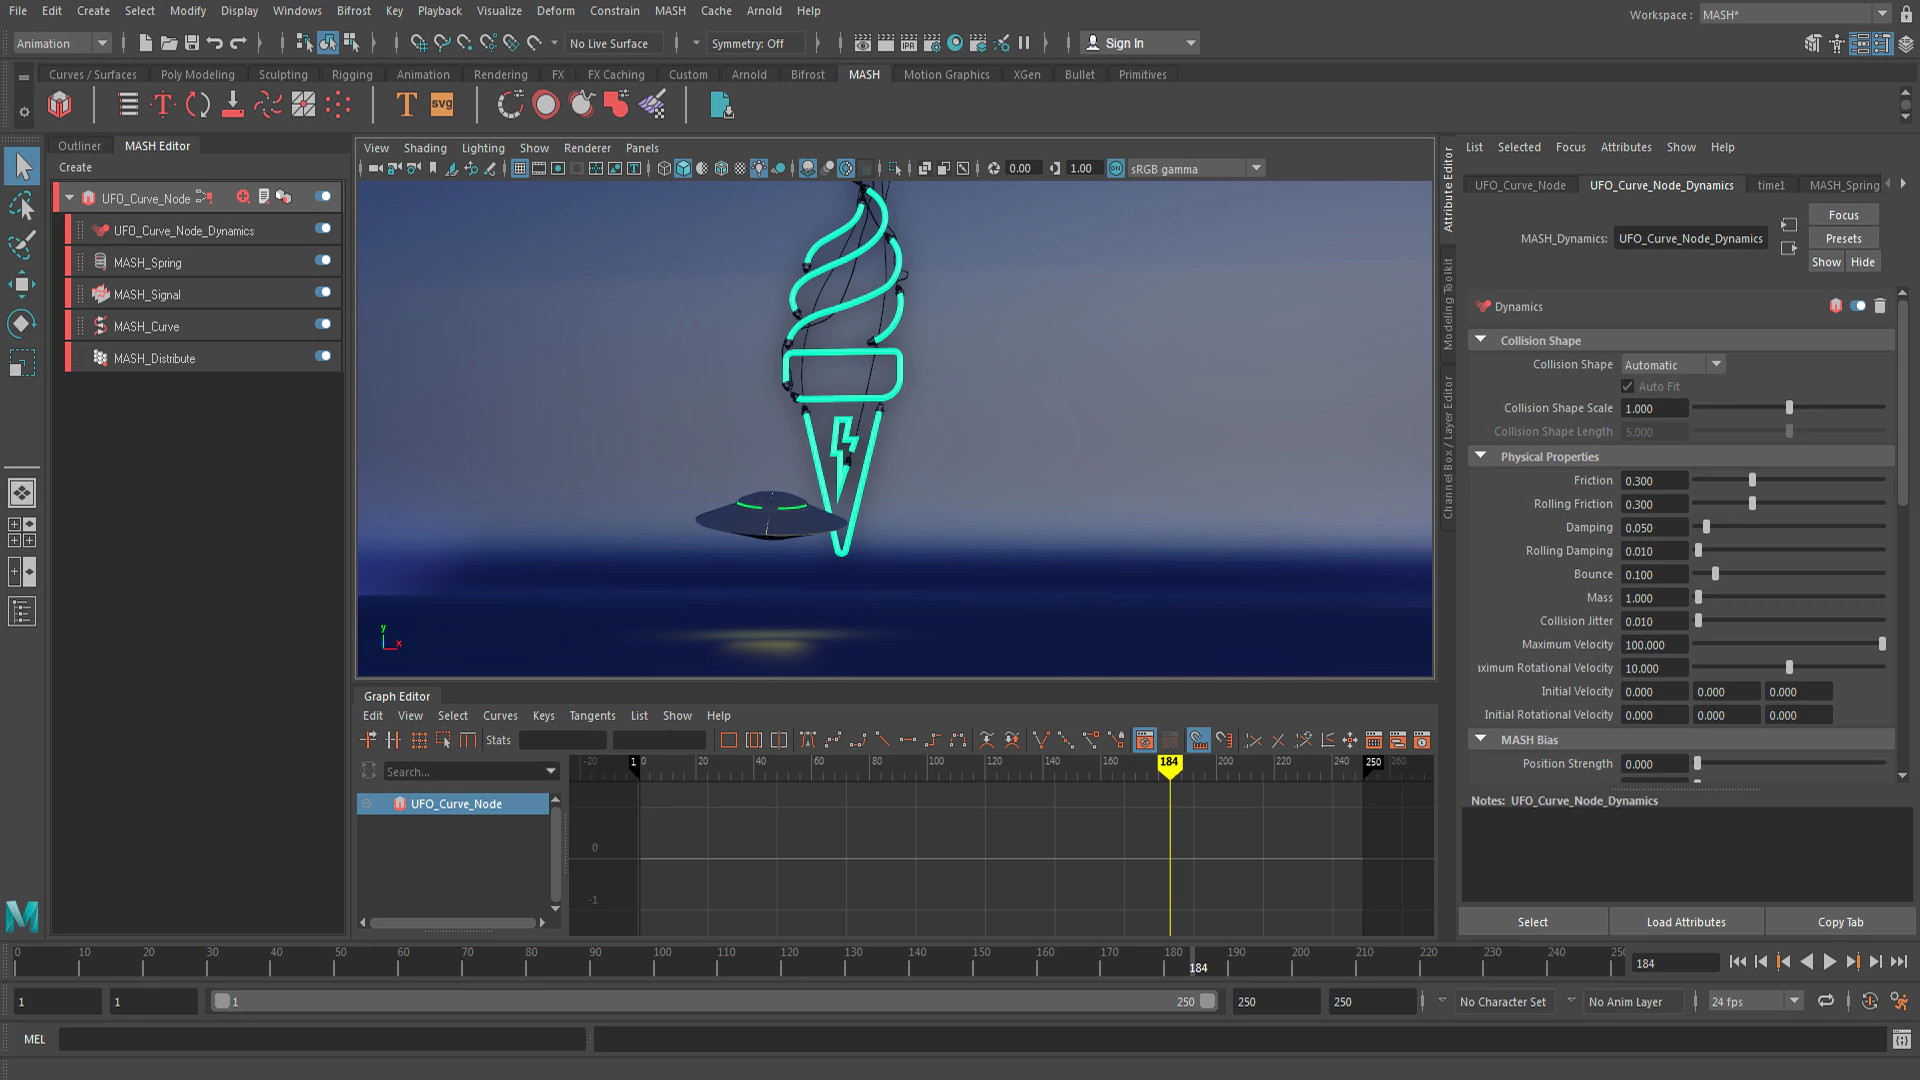
\includegraphics[width=0.9\textwidth]{imagenes/2/maya.jpg}
\caption{Captura de pantalla del entorno de trabajo de Maya}
\label{fig:maya}
\end{center}
\end{figure}

\subsubsection{Autodesk 3Ds Max}

Anteriormente 3D Studio Max, Autodesk 3Ds Max es un programa de creación de gráficos y animación 3D desarrollado por Autodesk, que lo compró a su anterior dueño por 182 millones de dólares. Actualmente es uno de los programas de animación 3D más utilizado, especialmente para el desarrollo de videojuegos, anuncios de televisión y arquitectura.

Todo empieza a mediados de los años 1980, con la creación del Grupo Yost. Este grupo estaba compuesto por varios expertos del sector que comenzaron a trabajar paralelamente en soluciones software que les permitieran trabajar con gráficos 3D. A finales de los 1980 decidieron unirlos en el el paquete \textit{The Cyber Studio}, al que poco a poco fueron añadiendo funcionalidades. Este programa no pasó desapercibido para la compañía Autodesk, dueña de AutoCAD, y al año siguiente contrataron a los principales desarrolladores de \textit{The Cyber Studio} para que trabajasen para ellos en su propio programa.

A principios del 1990 salió al mercado el programa 3D Studio, aunque no fue hasta 1996 cuando salió al mercado el 3D Studio Max, totalmente terminada y diseñada especialmente para Windows. Actualmente, en su versión 9 su nombre oficial Autodesk 3Ds Max.

\begin{figure}[!h]
\begin{center}
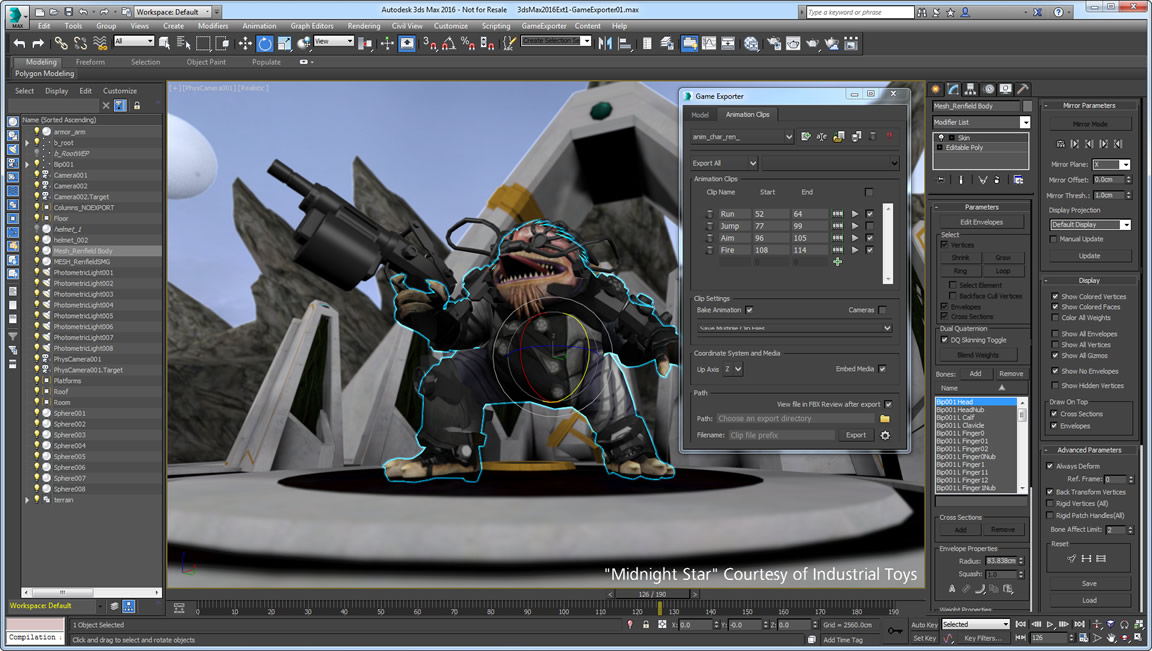
\includegraphics[width=0.9\textwidth]{imagenes/2/3ds-max.jpg}
\caption{Captura de pantalla del entorno de trabajo de 3Ds Max}
\label{fig:3ds-max}
\end{center}
\end{figure}

\subsection{Desarrollo}

Actualmente existen varios entornos de desarrollo integrado, o \acs{IDE} por sus siglas en inglés, destinados a facilitar el desarrollo de videojuegos. En esta sección se presenta los más importantes.

\subsubsection{Unity3D}

Unity es un motor de videojuego multiplataforma creado por Unity Technologies disponible para los principales sistemas operativos, y permite compilar para varias plataformas cómodamente. 

La compañía Unity Technologies fue fundada en 2004 en Dinamarca, la cual desarrolló Unity para su primer juego, \textit{GooBall}, que fue un fracaso. Aún así, los integrantes de la compañía reconocieron el valor del motor de juegos que había hecho y decidieron continuar con su desarrollo hasta lanzar oficialmente Unity un año después, en 2005.  

A día de hoy existen dos versiones; Unity Personal, una versión gratis de Unity para principiantes que no incluye servicio al cliente, capacitación ni servicios adicionales, y Unity Pro, que sí los incluye, costando 125\$ al mes. Además, los desarrolladores de un juego ingrese más de 100,000\$ al año deberán suscribirse a la versión Pro obligatoriamente. En total, más de cinco millones de personas han utilizado Unity en 2017\footnote{\url{https://unity3d.com/public-relations}}.

\begin{figure}[!h]
\begin{center}
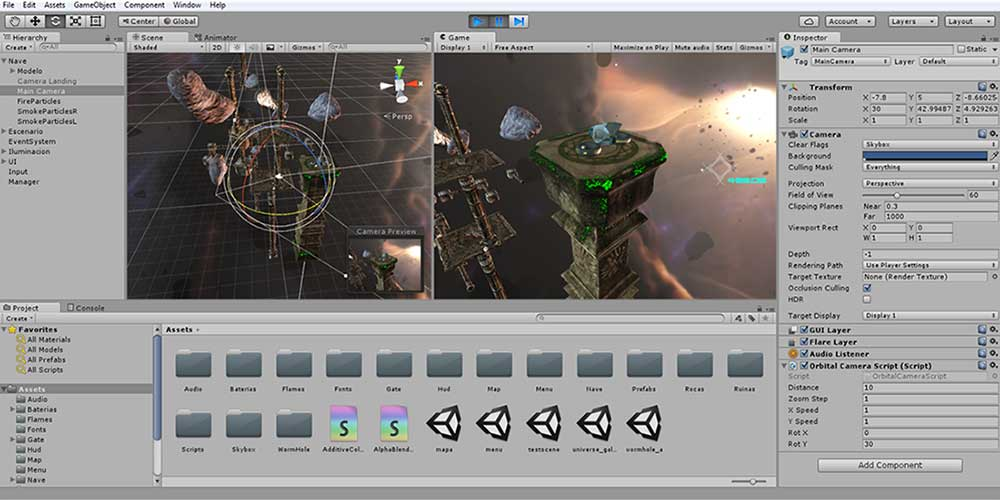
\includegraphics[width=0.9\textwidth]{imagenes/2/unity.jpg}
\caption{Captura de pantalla de un proyecto en Unity}
\label{fig:unity}
\end{center}
\end{figure}


\subsubsection{Unreal Engine}

Unreal Engine es un motor de juego creado por la compañía Epic Games que al estar escrito en C++ presenta un alto grado de portabilidad, por lo que es una de las herramientas más utilizadas por los desarrolladores de juegos.

Este motor fue mostrado inicialmente en el juego de disparos en primera persona \textit{Unreal} en 1998, que incluía detección de colisiones, IA y herramientas para trabajar con juegos en red. El motor se reescribió y cuatro años después se lanzó su segunda versión, que incluía físicas para vehículos y sistemas de partícula, además de soporte para PlayStation 2 y XBox.

Poco a poco, y gracias al éxito de este \acs{IDE}, a lo largo de los años ha ido aumentando sus características y añadiendo soporte para las tarjetas gráficas y videoconsolas que han ido apareciendo.

Desde marzo de 2015 Unreal Engine 4 está disponible públicamente de forma gratuita aunque, si se decide comercializar el juego, la desarrolladora deberá aportar el 5\% de los ingresos que obtenga a Epic\footnote{\url{https://www.unrealengine.com}}.

\begin{figure}[!h]
\begin{center}
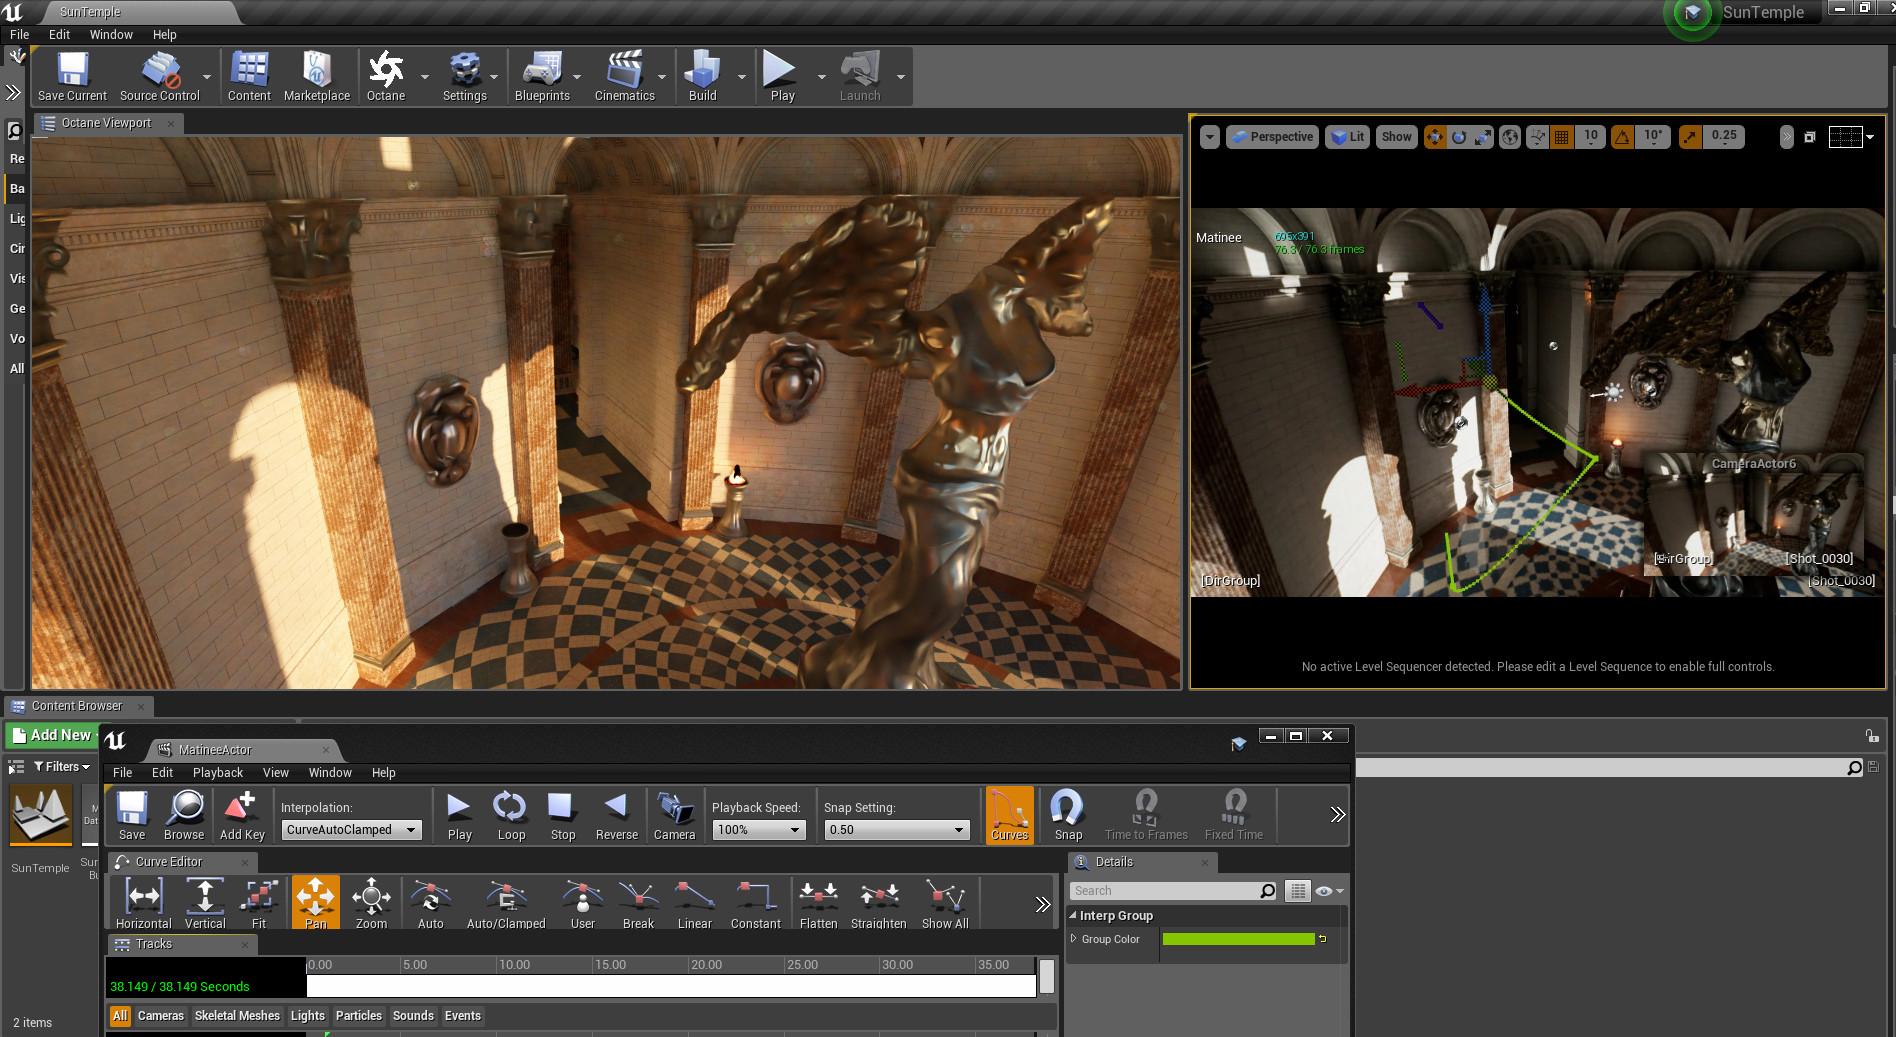
\includegraphics[width=0.9\textwidth]{imagenes/2/unreal-engine-4.jpg}
\caption{Captura de pantalla de un proyecto en Unreal Engine}
\label{fig:unreal}
\end{center}
\end{figure}

\subsubsection{Godot}

Godot es un motor de videojuegos 2D y 3D \textit{open source} publicado bajo la licencia \acs{MIT} desarrollado por su comunidad y disponible para los principales sistemas operativos.

Godot fue desarrollado y utilizado privativamente por la empresa argentina OKAM Studios desde principios del 2001, aunque en febrero de 2014 su código fuente fue liberado y publicado en GitHub\footnote{\url{https://github.com/godotengine/godot}}. Es el principal motor de videojuegos \textit{open source}, y su comunidad ayuda activamente a desarrollarlo. 

Además, actualmente tiene una página en Patreon\footnote{\url{https://www.patreon.com/godotengine}} con más de 1,000 mecenas y obtiene más de 10,000\$ al mes.

\begin{figure}[!h]
\begin{center}
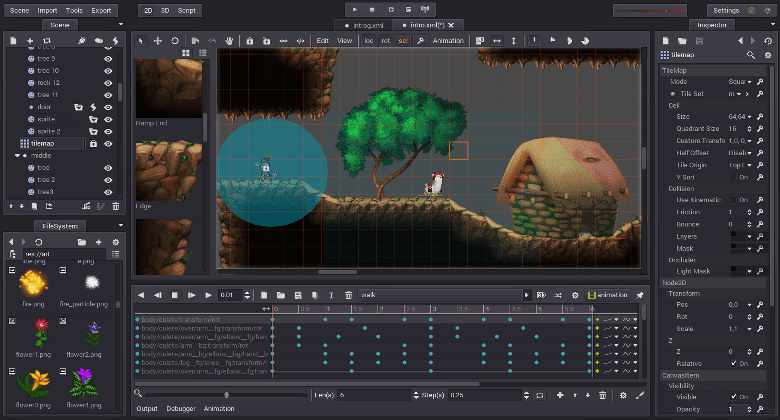
\includegraphics[width=0.9\textwidth]{imagenes/2/godot.jpg}
\caption{Captura de pantalla de un proyecto en Godot}
\label{fig:godot}
\end{center}
\end{figure}

\section{Desarrollo de videojuegos}

El desarrollo de videojuegos es el proceso de creación de un videojuego desde su concepción inicial hasta su versión final. Es una actividad multidisciplinar que involucra profesionales de distintos campos, como programadores, diseñadores gráficos, animadores o compositores de música, entre otras áreas.

A principios de la década de 1960 comenzaron a desarrollarse los primeros videojuegos, pero no estaban disponibles para el público general ya que éste no poseía dispositivos para ejecutarlos dado su elevado precio. No fue hasta la década de 1970 y la llegada de la primera generación de consolas de videojuegos y ordenadores domésticos, como el Apple I, cuando empezaron a desarrollarse videojuegos a nivel comercial. Además, como los ordenadores tenían muy poca potencia y los juegos eran muy simples, un único programador podía hacerse cargo del juego completo en no más de 6 meses \cite{next-gen-97}.

Sin embargo, la creciente potencia de procesamiento de los ordenadores, los estándares de la industria y las expectativas del jugador han hecho que esto deje de ser la norma y solo pase en casos aislados. El precio promedio de la producción de un videojuego lentamente aumentó de 1-4 millones de dólares en 2000 a más de 5 millones en 2005, y luego a más de 20 millones en 2010\footnote{\url{https://en.wikipedia.org/wiki/Video_game_development}}.

Uno de los documentos más importantes, si no el más, a la hora de desarrollar un videojuego es el \textbf{\acl{GDD}}, o por sus siglas en inglés \acs{GDD} a partir de ahora. Este es un documento creado y editado por el equipo de desarrollo  del juego y contiene toda la descripción del videojuego y se utiliza para organizar esfuerzos dentro de un equipo de desarrollo. Este documento no es el guión del juego, sino una síntesis que propone lo que va a ser para que todo el mundo tenga la misma idea en mente \cite{bet-03}. Es equivalente a la \textbf{Biblia} de una serie de televisión. 

Como podemos ver, el desarrollo de un videojuego ha ido adquiriendo un carácter mucho más formal, por lo que que se necesita coordinar a muchos profesionales teniendo en cuenta salarios y tiempos para que el producto final pueda generarse correctamente. En el capítulo \ref{chap:metodologias} se discutirá en mayor profundidad las actuales metodologías de desarrollo que existen y cómo se ha adaptado este proyecto a ellas.

\section{Conclusiones}

A lo largo de este capítulo se han presentado las principales áreas y tecnologías en las que se ha basado este proyecto y que deberán trabajar conjuntamente y hacer sinergia para su correcta completitud.

El papel de la Historia del Arte es principal en este proyecto; tanto su temática como su narrativa están estrechamente a este área, y la estética de cada una de las salas se verá altamente influenciada por la etapa artística que representa.

Por otro lado, el componente inmersivo de la Realidad Virtual es de esencial importancia, y se utilizará junto a la naturaleza motivadora de los videojuegos para hacer que todos los usuarios se sientan totalmente inmersos en el mundo virtual que les ofrece \textit{MineRVa}. Este mundo será modelado completamente a mano, por lo que la  utilización de técnicas y tecnologías de diseño 3D es de vital importancia.
\chapter{Análisis inicial del problema}
\label{chap:analisis_problema}

En este capítulo se presenta el nacimiento y la idea inicial de la que parte este proyecto, así como su narrativa y la descripción del mundo virtual en el que tiene lugar.

\section{Concepto inicial}

Lo primero que se hizo antes de empezar a trabajar en el proyecto fue proponer una narrativa en la que basar el diseño y desarrollo; por ello, el primer paso que se dio en el proyecto fue redactar el documento \textbf{Guía de salas}, que puede verse en el apéndice \ref{anexo:guia-salas}. En este documento se redactó la primera versión de la narrativa del juego además de una propuesta con las salas que habría en el museo y qué obras de arte y puzzles tendría cada una. Este documento  fue enviado al tutor de este \acs{TFM} y, tras él dar el visto bueno al mismo, se comenzó a trabajar en el proyecto

Además, como se está trabajando siguiendo una metodología enmarcada en el desarrollo de videojuegos, como se explica en profundidad en el capítulo \ref{chap:metodologias}, el siguiente documento en el que se empezó a trabajar y que sirvió de andamio para el proyecto fue el \textbf{\acl{GDD}}, o \acs{GDD}. En un desarrollo real, este documento contendría la información necesaria para que todos los integrantes del proyecto tuvieran clara la idea global del juego, y en este caso es lo mismo; el documento contiene, entre otra información, el resumen, los objetivos o la narrativa del juego, y puede consultarse en el anexo \ref{anexo:gdd}.

En resumen, \MineRVa es un juego con una historia de un jugador ambientado en un museo compuesto por varias habitaciones ambientadas en las principales épocas históricas con diferentes pruebas que el jugador tiene que superar para completar.

\section{Narrativa}

La narrativa del proyecto ha intentado ser enmarcada en un museo creíble y realista, de tal manera que se ha colocado al jugador en la piel de un detective infalible que ha sido contratado por el museo para resolver el misterio de la desaparición de su mayor obra de arte, y todo apunta a que ha sido robado. Este museo es el más grande del mundo y tiene obras de arte de todos los rincones, desde cuadros a estatuas.

El encargado de recibir al jugador en el museo es su vigilante, un vetusto y campechano señor que ha pasado toda su vida trabajando en él. Este personaje será el encargado de introducir al jugador la historia y las mecánicas del juego, de explicarle su misión y de guiarle a través de las distintas salas, ayudándole para que no se quede atascado.

Pero cuál es la sorpresa del jugador cuando, tras completar todas las pruebas y llegar al final del museo, descubre que ha sido el propio vigilante quien ha robado el cuadro para su disfrute personal.

\section{Mundo virtual}

A continuación se describirán la estética y la composición del mundo virtual de este proyecto.

\subsection{Estética}

Como el presupuesto de este proyecto es nulo y el tiempo disponible para completarlo es especialmente bajo, la estética deberá ser acorde a estos factores. Por ello, se ha elegido una \textbf{estética low poly}, con lo que los tiempos de modelado se verán muy reducidos. Aún así, se intentará que no sea especialmente plana con la ayuda de texturas medianamente realistas que ayuden a los jugadores a conseguir una mayor inmersión y a dar mayor personalidad a las salas, pero todas ellas deberán ser gratuitas.

Por otro lado, aunque el modelado de las salas deberá ser hecho manualmente, se podrán importar de internet modelos tridimensionales especialmente complejos, como las estatuas que se crean necesarias para las salas; estos modelos suelen ser digitalizaciones exactas, que se adaptarán para reducir el número de polígonos, reducir el peso total del juego y hacer que no sea necesario un equipo hardware potente para jugarlo.

\subsection{Descripción de las salas}

Cuando se habla de salas en este proyecto se refiere a las unidades que presentan una historia, una temática y un puzzle distinto a las demás. El museo estará compuesto por 7 salas, aparte de la de tutorial, y cada una de ellas hará referencia a un período artístico distinto y estará ambientada  decorada de manera coherente con él.

Aunque inicialmente se planteó hacer bifurcaciones en los caminos que llevan a las salas de manera que el jugador pudiera elegir o incluso que tuviera que ir para atrás para acceder a alguna tras desbloquearla, finalmente se ha decidido hacer un museo lineal, principalmente porque se espera que sea más fácil para los jugadores, y porque tiene más sentido en el contexto de la ambientación temporal de las salas que vayan una después de otra.

El objetivo de cada nivel o sala será resolver el puzzle propuesto para acceder a la siguiente, además de que el usuario interactúe con las obras de arte y aprenda sobre ellas, ya que en alguno de los casos le será necesario.

Como se ha indicado antes, en total habrá \textbf{8 salas}. La primera a la que accede el jugador será la del \textbf{tutorial}, que tendrá un puzzle especialmente fácil para que el jugador se pueda centrar en entender el concepto, las mecánicas y los controles del juego.

Tras ella el jugador accederá a la sala corresponderá al período \textbf{gótico-flamenco}, el primero desde el que se ha decidido trabajar y estará ambientado en el interior de una iglesia gótica, con paredes de piedra altas y bóvedas de crucería. Además, tendrá tres cuadros; a los lados, \textit{El Matrimonio Arnolfini} (1434)  de Jan van Eycky \textit{El descendimiento} de van der Weyden (1436), a modo representativo del género, y en la pared del fondo \textit{El jardín de las delicias} de El Bosco (alrededor del 1500), que se abrirá por la mitad para mostrar la puerta al siguiente nivel

La siguiente sala estará ambientada en el \textbf{renacimiento}, y tendrá ventanas amplias y frisos de marmol. Los cuadros de esta sala serán \textit{La última cena} de Leonardo da Vinci (alrededor de 1495), \textit{La escuela de atenas} de Rafael (1511) y \textit{La creación de Adán}, de Miguel Ángel Buonarroti (1511). Para ambientar la sala también se utilizarán esculturas 3D, como \textit{Piedad} o \textit{Moisés}, ambas de Miguel Ángel, ya modeladas y con licencias de uso libre.

A continuación se encontrará la sala del \textbf{barroco}, con altas paredes de piedra. El concepto de esta sala ha cambiado varias veces a lo largo del desarrollo del proyecto, y por cuadros finalmente se han utilizado cuatro cuadros de San Sebastián, que fue un santo al que asetearon hasta la muerte y del que se hicieron muchas versiones a lo largo de este período. Los pintores elegidos han sido será de Guido Reni (1625),  José de Ribera (1636), Mattia Preti (1657) y Peter Paul Rubens (1614).

La siguiente sala corresponderá al \textbf{romanticismo}, por lo que se habrá poca iluminación y se utilizarán texturas de madera y un sistema de partículas de niebla para crear inmersividad. Los cuadros elegidos han sido \textit{Fusilamiento de Torrijos y sus compañeros en las playas de Málaga} de Antonio Gisbert Pérez (1887), \textit{Doña Juana la Loca} de Francisco Pradilla y Ortiz (1877) y \textit{El caminante sobre un mar de nubes} de Caspar David Friedrich (1818).

La última sala estará ambientada en las \textbf{vanguardias del siglo XX}. Aunque en este período coexisten multitud de estilos distintos, se han elegido el \textbf{cubismo}, el \textbf{surrealismo} y el \textbf{postimpresionismo} como los más representativos, por lo que los cuadros utilizados para esta sala son, respectivamente, el \textit{Guernica} de Pablo Picasso (1937), \textit{La tentación de San Antonio} de Salvador Dalí (1946) y \textit{La noche estrellada} de Vincent van Gogh (1889).

Cuando el jugador complete todas las salas podrá acceder a la \textbf{sala final}, en la que descubrirá que el vigilante que creía su amigo es en realidad el ladrón de guante blanco al que ha estado persiguiendo desde el principio.

\chapter{Tecnologías y recursos}
\label{chap:tecnologia}

\section{Recursos}

\subsection{Recursos hardware}

\begin{itemize}
 \item \textbf{Lenovo Explorer.} Heatset VR
 \item \textbf{Asus R510V.}
\end{itemize}

\subsection{Recursos software}

\subsubsection{Sistema Operativo}

Windows 10 Edutation 

\subsubsection{Principales librerías}

Añadir imágenes

\begin{itemize}
    \item \textbf{SteamVR.}
    \item \textbf{Windows Mixed Reality for SteamVR.}
    \item \textbf{VRTK.}\footnote{\url{https://vrtoolkit.readme.io}} es un framework de desarrollo multilibrería desarrollado en solitario por \textit{TheStoneFox}\footnote{\url{https://github.com/thestonefox}} (no se ha conseguido encontrar su nombre verdadero), un hombre residente en Birmingham, Reino Unido.
\end{itemize}

\subsubsection{Herramientas de desarrollo}

\begin{itemize}
    \item \textbf{Unity3D} \texttt{C\#}
    \item \textbf{Blender} 2.79c opensource
    \item \textbf{Visual Studio Community} Desarrollado por Microsoft
    \item \textbf{Atom} Desarrollado por GitHub
    \item \textbf{Git} Herramienta de control de versiones
\end{itemize}

\subsubsection{Herramientas de documentación}

\begin{itemize}
    \item \textbf{\LaTeX.} Para la documentación final. Overleaf
    \item \textbf{LibreOffice Writer.} (v5.5) Para informes 
    \item \textbf{LibreOffice Draw.} (v5.5) Para generar diagramas vectoriales
    \item \textbf{LibreOffice Calc.} (v5.5) Para generar gráficas.
    \item \textbf{GIMP.} (v2.8.20)Para editar imágenes
    \item \textbf{Inkscape.} (v0.92)Para editar imágenes vectoriales.
\end{itemize}
\chapter{Metodologías}
\label{chap:metodologias}

\drop{H}{  ubo} un tiempo en el que desarrollar un juego no necesitaba mucho más de un equipo pequeño de personas (3 ó 4 como máximo) y no mucho más de 6 meses de esfuerzo \cite{dill-07}, pero la exacerbada competencia que existe actualmente en la industria implica equipos de desarrollo de más de 50 personas expertas trabajando durante varios años con un presupuesto de millones de dólares para lograr publicar un solo videojuego comercial \cite{mor-10}. 

Por tanto, dada la evidente complejidad tanto técnica como personal de un videojuego, es necesario manejar su desarrollo haciendo uso de las metodologías y técnicas de planificación adecuadas que involucren una serie de pasos organizados para guiar cada proceso hasta el resultado final; es decir, hacer un buen uso de la \textbf{Ingeniería del Software}. Según describe el ingeniero americano Barry Bohem en \cite{Boe-79}, un artículo de referencia en este campo, la Ingeniería del Software es \textit{the practical application of scientific knowledge to the design and the construction of computer programs and the associated documentation required to develop, operate and maintain them}.

Tras leer esta definición es fácil darse cuenta de lo fundamental que es llevar a cabo un diseño e implementación adecuados. En este capítulo se hablará de la metodología de desarrollo de videojuegos más común y a continuación se presenta y justificará la metodología de trabajo seguida a lo largo del desarrollo de \textit{MineRVa}.

\section{Metodologías de desarrollo de videojuegos}

Los videojuegos no dejan de ser un recurso informático, aunque están muy próximos en cuanto a consumo y producción al entorno audiovisual. El sistema de producción audiovisual tiene clara relación con gran parte de las fases de desarrollo del videojuego pero, a pesar de ser considerado un software más, no existe una metodología común y propia para su diseño y desarrollo \cite{man-14}. El campo del videojuego ya no es sólo una industria que aporta importantes beneficios sino que se convierte en objeto de estudio en lo que a metodologías se refiere \cite{agu-08}.

El desarrollo de un juego, a lo largo de su ciclo de vida, se puede asemejar al de una película de cine, pudiéndose segmentar en tres fases ampliamente diferenciadas: \textbf{pre-producción}, \textbf{producción} y \textbf{post-producción}, cada una con sus etapas características \cite{bet-03}.

\vspace{0.4cm}

\begin{figure}[!h]
    \begin{center}
        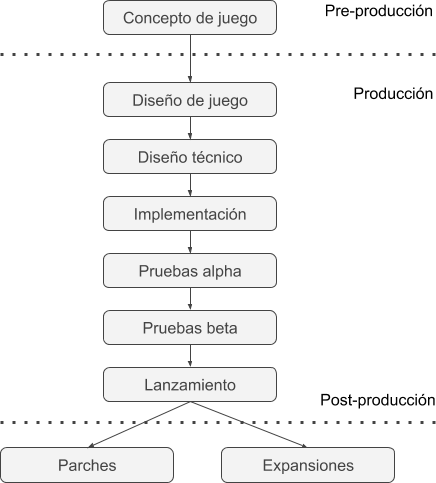
\includegraphics[width=0.625\textwidth]{imagenes/5/pre-prod-post.png}
        \caption{Fases del desarrollo de videojuegos, adaptado de \cite{man-14}}
        \label{fig:fases-desarrollo}
    \end{center}
\end{figure}

Esta metodología puede ser usada con distintos procesos de desarrollo, como \textit{Rational Unified Process}, \textit{Scrum} o \textit{Huddle}. Este último es un proceso específico de desarrollo de videojuegos y se llama así siguiendo la analogía de Scrum, ya que la reunión que se realiza en el fútbol americano antes de cada jugada se llama \textit{huddle}. Su filosofía es que mediante breves reuniones se planifique cada iteración, permitiendo tanto realizar un seguimiento más específico al avance del proyecto como poder hacer correcciones tempranas ante posibles desviaciones \cite{mor-10}.

Aunque el problema de proyectos privativos como videojuegos a gran escala es que no suele filtrarse mucha información referente a su parte técnica, sí se sabe que uno de los procesos más populares ha sido el de Cascada, aunque poco a poco las compañías han ido migrando a metodologías de desarrollo ágiles, más flexibles \cite{mor-10}.

A continuación se explican estas fases con más profundidad.

\subsection{Fase de pre-producción}

En la primera fase del proyecto se define el concepto de juego que estamos buscando así como sus aspectos más relevantes, como su \textbf{género}, su \textbf{historia} y sus principales \textbf{bocetos} para obtener una primera idea de su estilo \cite{rou-05}. Además, en esta fase se comienza a dar forma al \acs{GDD}, del que ya se habló en el capítulo \ref{chap:analisis_problema}.

\subsection{Fase de producción}

Esta es la fase más exigente del proyecto. En ella participan multitud de profesionales muy especializados y confluyen toda clase de actividades, como el diseño técnico, el diseño artístico o el diseño mecánico y la implementación y pruebas de los mismos. 

Además, a lo largo de esta fase se generan muchos documentos . Los más importantes son el \acs{GDD}, cuya finalización debería coincidir con la de esta fase, y la \textbf{Biblia del juego}, donde se recogen todas las historias de los personajes, del mundo donde sucede el juego, de su pasado y de los personajes secundarios que aparecen, creando el hilo argumental completo, con todos los detalles \cite{man-14}.

Esta fase termina con la generación del \textbf{gold master}, la copia definitiva que se envía a fábrica para su producción junto con el arte como la portada o el manual de usuario.

\subsection{Fase de post-producción}

Pero como ya sabemos el ciclo de vida de un producto software no termina con su entrega o, en este caso, su lanzamiento al mercado. Además de las tareas de marketing pertinentes, será preciso llevar a cabo un seguimiento adecuado para dar respuesta al comportamiento que el mercado ha tenido en relación al juego, ya que puede llegar a ser muy diferente al esperado.

Las tareas más inmediatas pueden ser parches para arreglar elementos o para ajustar su funcionamiento, y si nuestro juego contempla el lanzamiento de expansiones o DLCs (\textit{downloadable content}) también deberemos hacerlo en esta fase. Además, también deberá realizarse un \textbf{análisis post-portem} del proyecto para saber qué ha ido mal y poder mejorarlo para futuros proyectos.

Como puede verse, el desarrollo de un videojuego es una tarea larga y extremadamente compleja en la que intervienen profesionales de todo tipo y que es orquestada por un equipo de dirección que se encarga de que todo vaya según lo planeado y otro equipo de financiación encargado de que el presupuesto de producción se cumpla \cite{man-14}.

\section{Metodología de trabajo}

Antes de presentar el proceso de desarrollo y la metodología de desarrollo utilizada en este proyecto se describirá lo que es cada uno.

Un Por otro lado, una \textbf{metodología de desarrollo} es una implementación específica de un proceso de desarrollo. es una representación abstracta de una metodología de desarrollo. Procesos de desarrollo como por ejemplo \acs{UDP} o \textit{Agile Development} son abstracciones que definen las actividades que deben realizarse, pero no especifican cómo realizarlas o cuál debería ser el resultado.

Por otro lado, una \textbf{metodología de desarrollo} es la implementación específica de un proceso de desarrollo. Ejemplos de eso son \acs{RUP}, \textit{eXtreme Programming} y \textit{Scrum}. No son completamente explícitos pero definen qué, cuándo y cómo hacer las cosas.

Una vez diferenciados ambos conceptos, se pasa a explicar el proceso y la metodología de desarrollo que ha seguido este \acs{TFM}.

\subsection{Proceso de desarrollo}

En vista de los requisitos de flexibilidad que propone, y que en un proyecto de esta naturaleza son especialmente importantes, se ha elegido seguir el \textbf{Agile Software Development}.

Los principios fundamentales que rigen el Desarrollo Ágil están expuestos en \textbf{The Manifesto for Agile Software Development}\footnote{\url{http://agilemanifesto.org/}}, que fue escrito en febrero de 2001 por diecisiete ingenieros de software que llegaron a un acuerdo acerca de los cuatro pilares básicos que definían la forma correcta de desarrollar software.

\begin{center}
\begin{tcolorbox}[sharp corners,  colframe=white]
\begin{enumerate}
    \item \textbf{Individuals and interactions} over processes and tools.
    \item \textbf{Working software} over comprehensive documentation.
    \item \textbf{Customer collaboration} over contract negotiation.
    \item \textbf{Responding to change} over following a plan.
\end{enumerate}
\end{tcolorbox}
\end{center}

La primera regla hace referencia a la importancia del factor humano y a su coordinación, y asigna un papel secundario a seguir la metodología del proyecto de manera invariable.

La segunda regla señala la necesidad de priorizar el software resultante y su funcionalidad y utilidad sobre una documentación exhaustiva del proyecto.

La tercera regla da a entender a la importancia de colaborar con el cliente tanto como sea posible, en lugar de firmar un documento estático al comienzo del proyecto que contenga todos sus requisitos y no aceptar nada que no apareciera inicialmente en él.

Por último, la cuarta regla se enfoca en tratar de tomar decisiones flexibles ante problemas repentinos y cambios no planificados, adaptando el proyecto a ellos, en lugar de tratar de seguir el plan inicial a toda costa.

Del mismo modo, se definieron \textbf{12 principios}\footnote{\url{http://agilemanifesto.org/principles.html}} explicando qué debe regir cada metodología de desarrollo de software que utiliza este proceso de desarrollo.

\subsection{Metodología de desarrollo}

Dadas las necesidades de desarrollo explicadas anteriormente, la metodología de desarrollo más cercana a ellas es \textbf{Scrum}. Scrum no es una técnica para la construcción de productos; en su lugar, es un marco en el que se pueden emplear varios procesos y técnicas. Por este motivo Scrum no es una metodología exclusiva de desarrollo de software, ya que puede aplicarse a otras áreas, se adapta muy bien y permite que el equipo sea flexible para abordar los problemas y lograr resultados de alto valor \cite{scrum-guide}.

El principal valor de Scrum es su alta adaptabilidad a los cambios, lo que permite que el equipo y la organización del proyecto respondan rápidamente a los nuevos requisitos. Estos enfoques serían imposibles aplicando otras metodologías, como por ejemplo la de desarrollo en cascada.

Scrum se basa en la teoría empírica de control de procesos, que afirma que el conocimiento proviene de la experiencia y la toma de decisiones basadas en lo que se conoce. Esta metodología se apoya en tres pilares básicos.

\begin{itemize}
    \item \textbf{Transparencia.} Cualquier acción significativo debe ser visible para cada persona en el proyecto. Solo de este modo se puede compartir una comprensión común de lo que está sucediendo en cualquier momento.
    
    \item \textbf{Inspección.} Los artefactos de Scrum deben ser inspeccionados para detectar resultados indeseados. Estas inspecciones serán más beneficiosas si son realizadas por inspectores cualificados y siempre que no sean tan frecuentes como para interferir en el trabajo.

    \item \textbf{Adaptación}. Scrum utiliza un enfoque iterativo e incremental para adaptarse a los cambios y para controlar los riesgos. Cuando se detecte un problema, estas adaptaciones se deben realizar lo antes posible para desviarse lo menos posible de la planificación inicial.
\end{itemize}

Etimológicamente, \textit{scrum} es un movimiento en Rugby en el que un equipo se reúne para actuar de manera coordinada para que el balón pase de un extremo del campo al otro opuesto. Por lo tanto, hasta el nombre de esta metodología apunta a la necesidad de trabajar como un equipo sincronizado y bien comunicado para lograr un objetivo común.

De esta manera, Scrum intenta evitar que haya momentos en que un miembro del equipo no sepa qué hacer o no aporte valor al desarrollo, aunque Dilbert, en la figura \ref{fig:dilbert}, no esté de acuerdo con esto.

\begin{figure}[!h]
\begin{center}
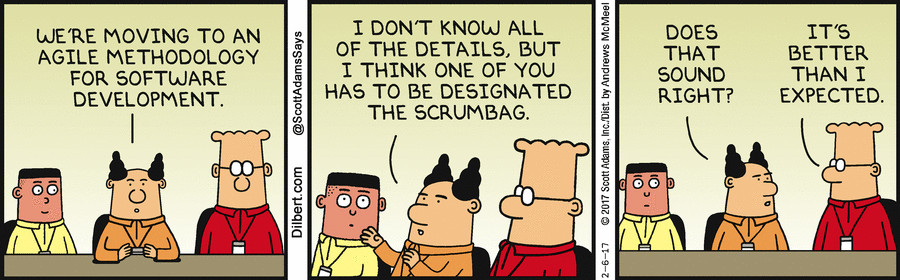
\includegraphics[width=0.95\textwidth]{imagenes/5/dilbert.jpg}
\caption{Dilbert y los roles de equipo, de \url{https://dilbert.com}}
\label{fig:dilbert}
\end{center}
\end{figure}

\subsubsection{Artefactos y eventos}

La figura \ref{fig:scrum} presenta una visión general de cómo funciona el flujo de trabajo de Scrum.

\begin{figure}[!h]
\begin{center}
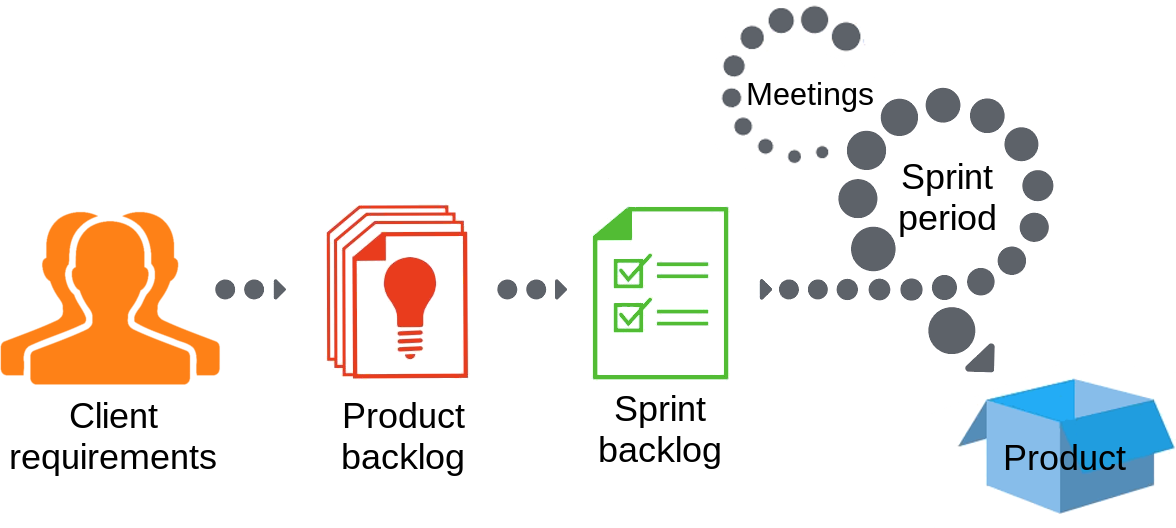
\includegraphics[width=0.95\textwidth]{imagenes/5/scrum.png}
\caption{Flujo de trabajo de Scrum, adaptado de \url{https://www.scrumalliance.org}}
\label{fig:scrum}
\end{center}
\end{figure}

Para poder explicar los roles de Scrum más claramente, primero se describirán brevemente los eventos que forman parte de esta metodología \cite{scrum-guide}.

\begin{itemize}
\item \textbf{Product backlog.} La cartera del producto es una abstracción que sirve para controlar las \textbf{historias de usuario} o \textit{user stories}. Éstas reflejan los requisitos que debe satisfacer el proyecto, que son establecidos por el cliente o el propietario del producto. 

Pero el \textit{product backlog} no solo permite agregar historias de usuarios, sino también todas las características, funciones y soluciones a las necesidades del proyecto. Cada uno de ellas estará formado por una descripción, una prioridad y el valor que agrega al producto. Además, se puede añadir el miembro Scrum asignado para completarla y cualquier observación relevante.

El \textit{product backlog} nunca se cierra, por lo que desde el inicio hasta el cierre del proyecto se pueden añadir nuevas historias de usuario o se pueden eliminar las que ya existen. Por lo tanto, a medida que el proyecto avanza la lista tiende crecen y alcanzan su máximo justo antes de la entrega final. Los requisitos nunca dejan de evolucionar, por lo que el \textit{product backlog} es un \textbf{objeto vivo}. Los cambios en los requisitos comerciales, las condiciones del mercado o la tecnología pueden hacer que cambie.
    
\item \textbf{Sprint.} El concepto clave de Scrum es un sprint, una \textbf{fase de trabajo} que dura un máximo de un mes, lo que genera un nuevo artefacto que puede ser potencialmente integrado en el producto final.

Se debe evitar que el tiempo del sprint sea demasiado largo, ya que de lo contrario la definición de lo que se está construyendo se vuelve demasiado amplia y la complejidad  y el riesgo aumentan.

Cada sprint puede considerarse un proyecto autocontenido, ya que se utilizan para lograr objetivos. Cada sprint tiene una definición de lo que se construirá, un diseño y un plan flexible que guiará su construcción y el artefacto resultante. Un nuevo sprint comienza inmediatamente después de que el anterior termine.

Un sprint está formado por varios eventos y artefactos.

\begin{itemize}

    \item [$\circ$] \textbf{Sprint period.} Es el período de tiempo que el sprint está destinado a durar.
        
    \item [$\circ$] \textbf{Sprint planning meeting.} Es una reunión dirigida por el \textbf{scrum master}, que debe asegurarse de que cada miembro haya entendido correctamente el resultado de la reunión.
    
    Esta reunión, que se lleva a cabo al comienzo de cada sprint, permite planear el trabajo a realizar de forma colaborativa por parte del equipo Scrum a partir del \textit{product backlog}.
    
    \item [$\circ$] \textbf{Sprint backlog.} Es un conjunto de elementos que pertenecen al \textit{product backlog} y que han sido \textbf{seleccionados para el sprint actual}. Es un pronóstico realizado por el equipo sobre qué funcionalidad estará en el próximo \textbf{incremento}. El \textit{sprint backlog} puede contener más de un solo elemento; de hecho, el equipo de Scrum añade los elementos identificados como necesarios para cumplir con el objetivo del sprint.
    
    Existen varias técnicas destinadas a lidiar con la necesidad de predecir cuánto puede durar una historia de usuario, como los \textbf{Mapa de afinidad} o el \textbf{Planning Poker}. Esta última es una técnica de estimación basada en el consenso dedicada a ayudar al equipo de desarrollo a tomar una decisión coordinada. Cada miembro hará una predicción en base a algunos valores prefijados y la representará el tiempo que cree que puede llevar terminar cada historia de usuario. Si todo el mundo coincide se dará por buena, pero si no se discutirá y se repetirá la votación hasta que todo el mundo coincida\footnote{\url{https://www.mountaingoatsoftware.com/agile/planning-poker}}.
        
    \item [$\circ$] \textbf{Daily Scrum.} Es un evento de 15 minutos para que el \textbf{equipo de desarrollo sincronice sus actividades} y cree un plan para el día actual. Esto se hace mirando el trabajo desde el último Scrum diario y prediciendo el trabajo que podría realizarse antes del siguiente. A lo largo de esta reunión, cada miembro del equipo responderá a tres preguntas:
    
    \begin{enumerate}
    \item ¿Qué hice ayer?
    \item ¿Qué voy a hacer hoy?
    \item ¿Creo que hay algo que está dificultando el desarrollo?
    \end{enumerate}
    
    De esa modo es muy fácil saber exactamente qué está haciendo cada miembro del equipo y detectar problemas emergentes.
    
     \item [$\circ$] \textbf{Sprint review.} Es una reunión informal que se lleva a cabo al final de cada sprint para \textbf{inspeccionar el trabajo realizado} y actualizar el \textit{product backlog}. La duración de ésta reunión suele ser directamente proporcional a la duración del sprint.
     
     \item [$\circ$] \textbf{Sprint retrospective.} Esta reunión se lleva a cabo después del \textit{sprint review} y antes de la planificación del próximo sprint, y ayuda al equipo de Scrum a inspeccionar el trabajo realizado y \textbf{detecte puntos débiles} antes del el próximo sprint.
        
\end{itemize}

\item \textbf{Product.} Es el motivo por el cual se desarrolla el proyecto; el artefacto final que se entregará al cliente.

\end{itemize}

\subsubsection{Flujo de trabajo y roles}

El marco trabajo de Scrum consta de varios roles; el \textbf{product owner} o propietario del producto, el \textbf{Scrum master} o maestro Scrum, \textbf{equipo de desarrollo} y los \textbf{stakeholders} o interesados, quienes juntos forman el \textbf{Scrum team}. Cada rol se relaciona con los otros por medio de varias actividades, eventos, interacciones y artefactos, y cada uno tiene un propósito específico y es esencial para el éxito del proyecto. Estas funciones y sus interacciones se muestran a continuación \cite{scrum-card}.

\begin{itemize}
\item \textbf{Product owner.} Es el responsable de \textbf{maximizar el valor del producto} coordinando correctamente las relaciones del Scrum team. Además, es el único responsable de administrar el \textit{product backlog}, lo que incluye,

\begin{itemize}
    \item[$\circ$] Definir las \textbf{historias de usuario}.
    \item[$\circ$] Ordenar las \textbf{historias de usuario} para alcanzar los objetivos de la mejor manera posible.
    \item[$\circ$] Asegurarse de que el \textit{product backlog} sea visible, transparente y \textbf{claro para todo el mundo}.
\end{itemize}

\item \textbf{Scrum master.} Es el responsable de garantizar que la \textbf{metodología Scrum sea entendida y aplicada por todo el mundo}. El Scrum master debe actuar como líder al servicio del equipo Scrum y ayudar a aumentar el valor de los artefactos que genere. 

El Scrum master puede ayudar a cada rol a maximizar su valor de varias maneras:
 
\begin{itemize}
    \item[$\circ$] \textbf{Al \textit{product owner}.} Su interacción principal con el este rol está dirigida a garantizar la gestión adecuada del \textit{product backlog}, haciendo que las historias de usuario sean lo más claras posible.
    
    \item[$\circ$] \textbf{Al equipo de desarrollo.} El Scrum master debe liderar al equipo de desarrollo y aumentar su efectividad para que generen productos de alto valor.
    
    \item[$\circ$] \textbf{A la organización.} El Scrum master debe ayudar a todas las partes interesadas a comprender y aplicar Scrum y trabajar con otros Scrum masters de otros equipos para aumentar la efectividad de la aplicación de esta metodología dentro de la organización.
    
\end{itemize}

\item \textbf{Equipo de desarrollo.} Que está formado por los desarrolladores que entregan el trabajo al cliente. Solo los miembros del equipo de desarrollo pueden crear el incrementos en el producto y decir que una historia de usuario se ha completado.

Estos desarrolladores son \textbf{auto-organizados} y \textbf{multi-función}. Además, Scrum no reconoce sub-equipos dentro del equipo de desarrollo. Aunque los miembros individuales pueden tener habilidades especializadas y áreas de enfoque, la responsabilidad del producto pertenece al equipo de desarrollo en su conjunto.

\item \textbf{Stakeholders.} Los interesados pueden ser individuos o empresas que se ven afectados por activa o por pasiva por el desarrollo del proyecto.

\end{itemize}

\section{Conclusiones}

Como se ha visto, las metodologías de desarrollo de videojuegos son complejas, ya que requieren la sincronización y el trabajo conjunto de muchos profesionales. Sin embargo, en este proyecto solo ha trabajado una persona, por lo que se han simplificado estas metodologías, adaptándolas a los requisitos del proyecto. Una de las principales ventajas de utilizar metodologías ágiles es esto mismo; poder modelar los procesos de desarrollo a las necesidades del proyecto a medida. 

Como en los entornos reales de desarrollo de videojuegos, este proyecto se ha desarrollo en torno a su \acs{GDD}, el documento que contiene toda su información, lo que significa que las iteraciones y el trabajo que conllevan se han basado en él.

Para ello, se ha diseñado un plan de entregas que guíe estas iteraciones y del que se hablará en el capítulo \ref{chap:plan_entregas}. Como se indica en Scrum, el final de cada iteración debe estar marcado por la generación de un entregable. Para probarlo, al final de cada iteración se grabará un vídeo mostrando los avances obtenidos a lo largo de la misma, que durará entre 4 y 6 minutos, y se subirá a YouTube. Además, en el capítulo \ref{chap:desarrollo}, que habla del desarrollo del proyecto a través de sus iteraciones, se mostrarán estos vídeos y se indicará su URL para que el lector pueda verlos y comprobar que su fecha de subida concuerda con la de su iteración.

Además, tanto el proyecto como su documentación se alojarán en repositorios de GitHub, cuyos respectivos enlaces son los siguientes.

\begin{center}
    \url{https://github.com/gomezportillo/mineRVa}
    \url{https://github.com/gomezportillo/mineRVa-doc}
\end{center}

\chapter{Plan de entregas}
\label{chap:plan_entregas}

\drop{E}{  n} cualquier proyectos es necesario planear de antemano las distintas iteraciones en las que se dividirá el trabajo, pero en los casos en los que se trabaja con nuevas tecnologías esto se vuelve esencial, ya que esto facilita el poder realizar un seguimiento del avance y la evolución del proyecto.

Un plan de entregas es un proceso que permite programar los distintos esfuerzos que se desarrollarán a lo largo de un proyecto, aportando  una visión global del mismo.

En este capítulo se presentará y desglosará el plan de entregas seguido para este \acs{TFM}. Primero se hará en forma de tabla, que se ha usado a lo largo del proyecto para facilitar su seguimiento, y luego se pasará a describir de las entregas en más profundidad.

De aquí en adelante se hablará de \textit{entrega} para definir el esfuerzo que genera un entregable y de \textit{iteración} para describir las subtareas en las que se han dividido cada una de las entregas.

\section{Plan de entregas}

En las tablas siguientes puede verse un resumen de las iteraciones y sus tareas, aunque en la sección posterior se explicarán con más detalle.

Al final de todas las entrega se perfilarán las salas anteriores con el fin de mejorarlas de manera progresiva; como siempre será así, se ha evitado incluir esta iteración en la siguiente tabla, además de grabar un vídeo enseñando los avances obtenidos y subirlo a YouTube. La lista de reproducción creada con todos los vídeos puede consultarse en el siguiente enlace.

\begin{center}
    \url{https://www.youtube.com/playlist?list=PLb5boRKcO4iapVxIHKnowO8E2WnaLylcT}
\end{center}

Por último, la iteración final estará centrada en realizar una evaluación del proyecto con usuarios reales quieres, tras completar el juego, responderán dos cuestionarios con el objetivo de conocer su grado de satisfacción con el juego y su eficacia para aprender los conceptos que se pretende enseñar.

% -------------------- Tabla 1

\vspace{1cm}

\begin{table}[H]
    \centering
    \begin{tabular}{p{.1\textwidth} p{.675\textwidth} p{.125\textwidth}}
\hline
\rowcolor{lightgray!30}
\textbf{Entrega} & 
\textbf{Objetivo} & 
\textbf{Deadline}

\\ \hline

0
& 
Tener una idea general de la narrativa del proyecto y tener un entorno de desarrollo configurado
\newline
\newline
\begin{tabular}{p{.01\textwidth} p{.55\textwidth}}
  \firsthline
  \multicolumn{1}{l}{\textbf{Iter.}} &
  \multicolumn{1}{l}{\textbf{Descripción}} \\ \hline

  1 & Generar un documento con el prototipo de la narrativa \\ \hline
  2 & Configurar el entorno de desarrollo con las librerías seleccionadas y el headset VR proporcionado \\ \hline
  
  \end{tabular} 
\newline
&
15/2    

\\ \hline

1       
&
Tener dos salas que actúen como tutorial para los jugadores
\newline
\newline
\begin{tabular}{p{.01\textwidth} p{.55\textwidth}}
  \firsthline
  \multicolumn{1}{l}{\textbf{Iter.}} &
  \multicolumn{1}{l}{\textbf{Descripción}} \\ \hline

  1 & Modelar y texturizar la antesala al museo\\ \hline
  2 & Importarla a Unity correctamente\\ \hline
  3 & Dotar a la sala de físicas y colisiones\\ \hline
  4 & Conseguir que el jugador pueda moverse por ella\\ \hline
  5 & Repetirlo todo con la primera sala de tutorial\\ \hline
  6 & Modelar varias piezas de fruta y hacer que puedan ser cogidas y lanzadas\\ \hline
  7 & Hacer que el jugador pueda moverse entre salas \\ \hline
  \end{tabular} 
\newline
&
28/2

\\ \hline

\end{tabular}
\caption{Plan de entregas 0 y 1}
\label{tab:entregas1}
\end{table}

% -------------------- Tabla 2

\begin{table}[H]
    \centering
    \begin{tabular}{p{.1\textwidth} p{.675\textwidth} p{.125\textwidth}}
\hline
\rowcolor{lightgray!30}
\textbf{Entrega} & 
\textbf{Objetivo} & 
\textbf{Deadline}

\\ \hline

2       
&
Tener terminada la segunda sala, ambientada en el Gótico
\newline
\newline
\begin{tabular}{p{.01\textwidth} p{.55\textwidth}}
  \firsthline
  \multicolumn{1}{l}{\textbf{Iter.}} &
  \multicolumn{1}{l}{\textbf{Descripción}} \\ \hline

  1 & Modelar, texturizar e importar la segunda sala\\ \hline
  2 & Modelar la palanca y hacer que desbloquee la puerta de salida \\ \hline
  3 & Comenzar a trabajar en la siguiente sala \\ \hline
  4 & Hacer que cuando un objeto toque el suelo vuelva a su posición original \\ \hline
  \end{tabular} 
\newline
&
15/3

\\ \hline

3       
&
Tener terminada la tercera sala, ambientada en el Renacimiento, el prototipo un sistema de interacción avanzado y desarrollar tareas menores
\newline
\newline
\begin{tabular}{p{.01\textwidth} p{.55\textwidth}}
  \firsthline
  \multicolumn{1}{l}{\textbf{Iter.}} &
  \multicolumn{1}{l}{\textbf{Descripción}} \\ \hline

  1 & Terminar de modelar la tercera sala\\ \hline
  2 & Implementar el sistema/puzzle que haga que se abra la puerta\\ \hline
  3 & Elegir qué sistema de interacción se va a hacer para la siguiente sala\\ \hline
  4 & Desarrollar un prototipo funcional preparado para ser importado a la siguiente sala\\ \hline
  5 & Mostrar la descripción de los cuadros al pulsar un botón \\ \hline
  6 & Hacer un fundido a negro al cambiar de sala \\ \hline
  \end{tabular} 
\newline
&
31/3

\\ \hline

4       
&
Completar la cuarta sala, ambientada en el Barroco, comenzar a trabajar en la quinta y seguir trabajando en tareas menores
\newline
\newline
\begin{tabular}{p{.01\textwidth} p{.55\textwidth}}
  \firsthline
  \multicolumn{1}{l}{\textbf{Iter.}} &
  \multicolumn{1}{l}{\textbf{Descripción}} \\ \hline

  1 & Modelar y texturizar la cuarta sala\\ \hline
  2 & Importar el sistema de interacción avanzado\\ \hline
  3 & Integrarlo en la sala para obtener un puzzle interesante\\ \hline
  4 & Comenzar a modelar la quinta sala\\ \hline
  5 & Añadir un candado a las puertas bloqueadas que desaparezca al abrirlas \\ \hline
  \end{tabular} 
\newline
&
30/4

\\ \hline

\end{tabular}
\caption{Plan de entregas 2, 3 y 4}
\label{tab:entregas2}
\end{table}

% -------------------- Tabla 3

\begin{table}[H]
    \centering
    \begin{tabular}{p{.1\textwidth} p{.675\textwidth} p{.125\textwidth}}
\hline
\rowcolor{lightgray!30}
\textbf{Entrega} & 
\textbf{Objetivo} & 
\textbf{Deadline}

\\ \hline

5       
&
Terminar la quinta sala, ambientada en el Romanticismo, y la sexta, ambientada en las Vanguardias
\newline
\newline
\begin{tabular}{p{.01\textwidth} p{.55\textwidth}}
  \firsthline
  \multicolumn{1}{l}{\textbf{Iter.}} &
  \multicolumn{1}{l}{\textbf{Descripción}} \\ \hline

  1 & Completar el modelado la quinta sala\\ \hline
  2 & Desarrollar un sistema de partículas que imiten neblina ambiental\\ \hline
  3 & Diseñar e integrar un acertijo con alguna interacción interesante\\ \hline
  4 & Modelar la sexta sala\\ \hline
  5 & Integrar un puzzle que tenga que ser completado con las piezas de los cuadros elegidos\\ \hline
  \end{tabular} 
\newline
&
15/6

\\ \hline

6       
&
Diseñar y modelar la séptima, el almacén del vigilante y la sala final e integrar el resto de elementos restantes como diálogos
\newline
\newline
\begin{tabular}{p{.01\textwidth} p{.55\textwidth}}
  \firsthline
  \multicolumn{1}{l}{\textbf{Iter.}} &
  \multicolumn{1}{l}{\textbf{Descripción}} \\ \hline

  1 & Modelar la séptima sala y elegir el cuadro robado\\ \hline
  2 & Modelar la última sala\\ \hline
  3 & Incluir un modelo del vigilante, añadirle animaciones e integrarlas con el juego\\ \hline
  4 & Desarrollar un sistema de diálogos\\ \hline
  5 & Añadir las descripciones al resto de cuadros\\ \hline
  6 & Desarrollar un menú de juego inicial\\ \hline
  7 & Añadir música de fondo y efectos de sonido\\ \hline
  \end{tabular} 
\newline
&
25/6

\\ \hline

\end{tabular}
\caption{Plan de entregas 5 y 6}
\label{tab:entregas3}
\end{table}

% -------------------- Tabla 4

\begin{table}[H]
    \centering
    \begin{tabular}{p{.1\textwidth} p{.675\textwidth} p{.125\textwidth}}
\hline
\rowcolor{lightgray!30}
\textbf{Entrega} & 
\textbf{Objetivo} & 
\textbf{Deadline}

\\ \hline

7       
&
Terminar la documentación y generar un tráiler y un vídeo mostrando todo el juego
\newline
\newline
\begin{tabular}{p{.01\textwidth} p{.55\textwidth}}
  \firsthline
  \multicolumn{1}{l}{\textbf{Iter.}} &
  \multicolumn{1}{l}{\textbf{Descripción}} \\ \hline

  1 & Realizar una evaluación del juego final con usuarios reales\\ \hline
  2 & Grabar un vídeo mostrando todo el juego\\ \hline
  3 & Grabar y editar un tráiler de ~90 segundos de duración\\ \hline
  4 & Terminar de redactar y maquetar la documentación\\ \hline
  5 & Realizar la presentación para la defensa con tribunal\\ \hline
  \end{tabular} 
\newline
&
11/7

\\ \hline

\end{tabular}
\caption{Plan de entrega 7}
\label{tab:entregas4}
\end{table}


\section{Descripción de las entregas}


El desarrollo del proyecto ha sigo guiado por un total de 7 entregas, cada una subdividida a su vez en una o varias iteraciones. El resultado de cada una de las entregas ha sido un entregable, permitiendo de este modo realizar un seguimiento preciso del desarrollo del proyecto.

Además, al final de cada entrega se generará un vídeo de entre 4 y 6 minutos mostrando los avances obtenidos a lo largo de la misma y que será subido a la plataforma YouTube. Al final de la descripción del desarrollo de cada entrega, en el capítulo \ref{chap:desarrollo}, se indicarán los enlaces  a cada uno de ellos.

El proyecto se inició a principios del segundo semestre y se planeó terminar a finales de junio, por lo que las fechas de las entregas se deberán ajustar para no sobrepasarlas. Además, se intentará que cada una dure aproximadamente dos semanas, ya que es un tiempo razonable para, aun compaginando el desarrollo de este proyecto con las seis asignaturas del segundo semestre, generar un entregable con el suficiente valor como para marcar el final de la entrega.

Por otro lado, y paralelamente a las entregas, se trabajará en esta documentación para que pueda ser terminada prácticamente al mismo tiempo que el desarrollo software.

\subsection{Entrega 0}

Se utilizará la primera entrega del proyecto como toma de contacto con el entorno de desarrollo, las tecnologías a utilizar y el proyecto en sí.

Como tareas se definirán generar un primer prototipo de la narrativa del proyecto enmarcándola en un museo creíble y realista y configurar el \acs{IDE} y las librerías.

Los entregables resultantes de esta entrega serán, por un lado, un documento describiendo la narrativa y la estructura de salas del museo, y por el otro un proyecto Unity adecuadamente configurado que se pueda ejecutar con el headset \acs{VR} proporcionadas y en el que el jugador pueda moverse de manera adecuada.

\begin{itemize}
    \item \textbf{Fecha de inicio.} 1 de febrero de 2019
    \item \textbf{Fecha de fin.} 15 de febrero de 2019
\end{itemize}

\subsection{Entrega 1}

Una vez que el contamos con una narrativa de la que partir y un entorno de desarrollo correctamente configurado, el objetivo principal de la la siguiente entrega será aprender a exportar correctamente modelos 3D de Blender a Unity y a trabajar de un modo básico con el framework \acs{VRTK}.

Esta entrega tendrá varias iteraciones; primero, modelar una antesala al museo relativamente simple en Blender, aplicarle materiales y texturas y aprender a importar todo correctamente desde Unity y una vez conseguido, el siguiente paso será configurar la escena para dotarla de físicas y colisiones para que al iniciar el juego el jugador pueda moverse por ella de un modo similar a como lo haría en una habitación real.

Siguiendo con las salas, y una vez aprendido cómo exportarlas al motor del juego, se modelará la sala que actuará como tutorial al juego y a sus dinámicas y se modelarán y configurarán un par de piezas de fruta con las que el usuario pueda interactuar; cogerlas y soltarlas encima de otros modelos e incluso lanzarlas y que estas se comporten de manera orgánica.

El resultado de esta entrega será una versión del proyecto con las dos salas explicadas anteriormente y que permita al usuario moverse entre ellas.

\begin{itemize}
    \item \textbf{Fecha de inicio.} 16 de febrero de 2019
    \item \textbf{Fecha de fin.} 28 de febrero de 2019
\end{itemize}

\subsection{Entrega 2}

La siguiente entrega consistirá en seguir aprendiendo a trabajar con el framework elegido, permitiendo realizar tareas inicialmente más difíciles como mover objetos programáticamente haciendo uso del framework de \acs{VR}.

En lo que respecta a sus iteraciones, y como la siguiente sala a modelar, ambientada en el gótico y la primera temática del museo, consta de muchos detalles y técnicas más avanzadas de modelado, y por tanto se espera dedicar más tiempo en este trabajo, será la única que se modelará. Por otro lado, se volverá a las dos primeras salas ya modeladas para terminarlas y mejorar su apartado gráfico. Además, si sobra tiempo, se comenzará a modelar la siguiente sala.

El entregable por tanto, será una versión del proyecto en la que se puede hacer uso de aspectos más avanzados de las librerías utilizadas para permitir al usuario interactuar con modelos tridimensionales que actúen como interfaces para controlar otros elementos. Siguiendo con el documento inicial, se conseguirá abrir y cerrar una puerta corredera a la que inicialmente el jugador no tiene acceso interactuando con una palanca.

\begin{itemize}
    \item \textbf{Fecha de inicio.} 1 de marzo de 2019
    \item \textbf{Fecha de fin.} 15 de marzo de 2019
\end{itemize}

\subsection{Entrega 3}

La tercera entrega del proyecto pretende ser algo más práctica. Una vez teniendo más soltura con el framework y el entorno de desarrollo, se valorará la inclusión de técnicas de interacción mucho más avanzadas, que quizá en un principio por falta de experiencia con las tecnologías y las librerías utilizadas ni siquiera se plantearon. Por ejemplo, se estudiará el incluir elementos como un arco o una pistola que el jugador pueda disparar para acertar a objetivos. Además, se trabajará en tareas que inicialmente podían resultar más difíciles como hacer un fundido a negro al cambiar de sala, mostrar la descripción de las obras de arte de las salas (que serán leídas desde un archivo en disco) con la interacción el jugador con los mandos o teletransportar un objeto de vuelta a su posición original si toca el suelo para que el jugador no tenga que agacharse a recogerlo.

Paralelamente, se seguirá trabajando en el resto de salas, perfilándolas, y terminado aquellos modelos dejados a medias.

El resultado de esta entrega, por lo tanto, serán las 4 salas anteriores prácticamente terminadas y un prototipo funcional con alguna técnica de interacción avanzada para la quinta.

\begin{itemize}
    \item \textbf{Fecha de inicio.} 15 de marzo de 2019
    \item \textbf{Fecha de fin.} 31 de marzo de 2019
\end{itemize}

\subsection{Entrega 4}

La cuarta entrega del proyecto partirá del prototipo desarrollado en la entrega anterior para modelar la siguiente sala del proyecto y dotarla de la lógica necesaria para que la interacción que se desarrolle en ella sea interesante y divertida para el jugador. Además, se comenzará a trabajar en la siguiente sala, la sexta, y se modelará su estructura básica.

El principal problema de esta entrega es que dadas las fechas en las que se desarrollará, previsiblemente se solapará con Semana Santa y los distintos trabajos de las asignaturas del máster, por lo que se le dotará del doble de tiempo para terminarla, es decir, un mes.

\begin{itemize}
    \item \textbf{Fecha de inicio.} 1 de abril de 2019
    \item \textbf{Fecha de fin.} 30 de abril de 2019
\end{itemize}

\subsection{Entrega 5}

En esta entrega, la quinta, se terminará de modelar la sala del Romanticismo y se completará el desarrollo de la prueba elegido. Tras ello, se diseñará, modelará y desarrollará de manera íntegra la sexta sala, ambientada en las Vanguardias.

Por tanto, el resultado de esta entrega será una versión jugable del proyecto con todas las salas ambientadas y sus pruebas finalizadas.

Debido a la fecha en la que deberá realizarse, esta entrega coincidirá completamente con los exámenes y las entregas de los trabajos del máster; por ello, se le ha asignado más tiempo que al resto de entregas para poder ser completada correctamente.

\begin{itemize}
    \item \textbf{Fecha de inicio.} 1 de abril de 2019
    \item \textbf{Fecha de fin.} 7 de junio de 2019
\end{itemize}


\subsection{Entrega 6}

La sexta entrega del proyecto concluirá la parte software del proyecto; se deberá terminar el desenlace del juego, además de un pequeño epílogo para que el final no sea tan abrupto. Para ello, se incluirá el modelo de un vigilante con el que el jugador pueda interactuar, por lo que también se le añadirán animaciones y se desarrollará un sistema de diálogos. 

Para aumentar la sensación de realismo y de inmersión del jugador, se añadirá música de fondo diferente para cada sala, libre de derechos de autor, y efectos de sonido para algunas de las acciones que el jugador más realice. 

Además, se terminará de incluir las descripciones de las obras de arte que hay en el museo.

Por último, se trabajará en generar un menú inicial desde el que el jugador pueda empezar una partida, ver los créditos o salir del juego.

Aunque para estas fechas se deberá estar finalizado las clases y las entregas del máster, se deberá compaginar el desarrollo de este proyecto con las prácticas de empresa, por lo que se le ha asignado un tiempo de dos semanas, como a las entregas iniciales.

\begin{itemize}
    \item \textbf{Fecha de inicio.} 7 de junio de 2019
    \item \textbf{Fecha de fin.} 25 de junio de 2019
\end{itemize}


\subsection{Entrega 7}

Finalmente, la última entrega del proyecto se dedicará a completar la documentación restante y realizar una evaluación de satisfacción del juego final con usuarios reales. Esta evaluación se incluirá en la documentación y se usará como medida de aproximación a la satisfacción de los jugadores con respecto al proyecto. 

Además, se grabará un vídeo que muestre el juego completo, de inicio a fin, y se generará un pequeño tráiler, del estilo de un anuncio de televisión, que se usará para promocionar el juego.

Por último, se generará la presentación del proyecto que se utilizará en la defensa del \acs{TFM} y que resumirá esta documentación.

\begin{itemize}
    \item \textbf{Fecha de inicio.} 25 de junio de 2019
    \item \textbf{Fecha de fin.} 11 de julio de 2019
\end{itemize}
\chapter{Desarrollo}
\label{chap:desarrollo}

\drop{C}{  omo} ya se ha comentado antes, el desarrollo de este proyecto ha supuesto un reto importante ya que las tecnologías utilizadas eran totalmente desconocidas. En este capítulo se explica el proceso seguido a lo largo de su desarrollo, además de presentar los principales problemas encontrados y las soluciones con las que se han abordado.

\section{Entrega 0}

El objetivo de esta primera entrega fue, por un lado, establecer la estructura principal del proyecto y esbozar una primera versión del a narrativa y por otro realizar una primera toma de contacto con el desarrollo de Unity, las tecnologías \acs{VR} e instalar y configurar el entorno de desarrollo para poder empezar a trabajar en la siguiente entrega.

\subsection{Estructuración del proyecto}

El primer paso lógico tras proponer al tutor de este \acs{TFM} el proyecto y ser aprobado fue empezar a definirlo. Para ello, y partiendo de la idea principal de desarrollar una experiencia de juego haciendo uso de tecnologías \acs{VR} que pusiera en contacto con el mundo del arte a personas que suelen y no visitar museos, se generó el documento que puede verse en el anexo \ref{anexo:guia-salas}. 

Este documento comienza a detallar la narrativa del juego y la integra en una visita por un museo ficticio y, aunque terminó por sufrir varios cambios importantes, sirvió para definir el punto de partida del proyecto.

A lo largo de este documento se intenta crear una historia interesante para el jugador al mismo tiempo que generar un museo ficticio pero realista y coherente en el que se pueda desarrollar dicha narrativa. Para ello, se ha seguido el orden cronológico por las épocas más importantes en la historial de arte, definiendo una sala con una historia diferente para cada una.

A la hora de elegir los cuadros que se mostrarían en las salas se intentó buscar aquellos más representativos de su época. Para ello, se contó con el asesoramiento de una historiadora del arte, que ha sido quien ha dado el visto bueno al rigor artístico del museo y sus salas.

\subsection{Configuración del entorno de desarrollo}

Antes de poder empezar a desarrollar el proyecto fue necesario elegir un \acs{IDE} y un framework con el que trabajar. Como ya se ha explicado en los capítulos \ref{chap:estado_arte} y \ref{chap:tecnologia}, tras comparar las ventajas y desventajas de los entornos de desarrollo y librerías disponibles en el mercado se decidió trabajar con Unity, el framework \acs{VRTK} y la librería SteamVR para lo que, tras instalarlas, hubo que importarlas manualmente al proyecto de Unity.

\subsection{Primera toma de contacto con Unity}

A continuación se presenta un resumen de la interfaz de Unity par que el lector pueda entender algunos de los conceptos de los que se hablará más adelante.

\begin{figure}[!h]
\begin{center}
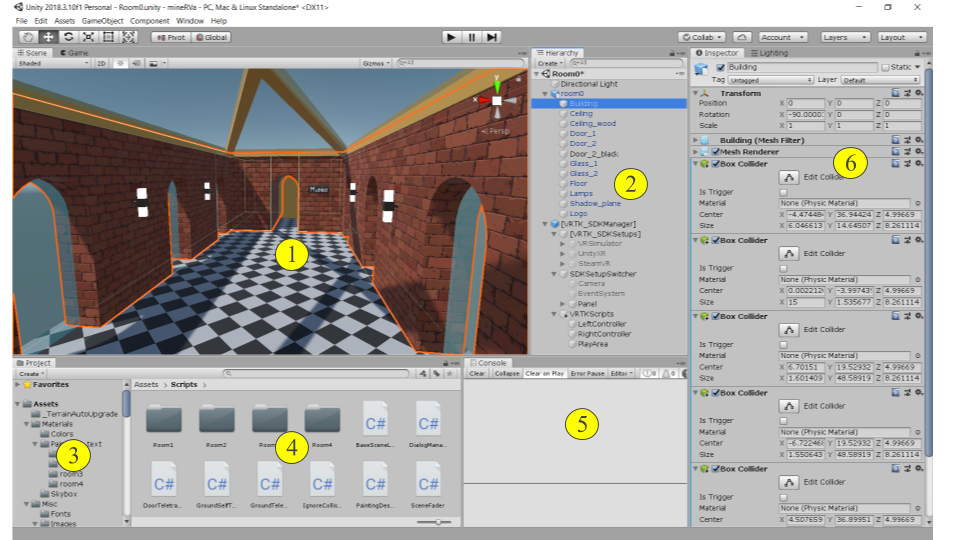
\includegraphics[width=1\textwidth]{imagenes/7/interfaz-unity.png}
\caption{Resumen de la interfaz de Unity}
\label{fig:interfaz-unity}
\end{center}
\end{figure}

\begin{enumerate}
    \item Vista de la escena actual, en la que el usuario puede obtener una vista previa de la escena e interactuar con los objetos tridimensionales para colocarlos. Funciona de manera parecida a Blender.
    
    \item Vista de la jerarquía de la escena, en la que pueden verse los objetos que hay y sus relaciones; por ejemplo, si están emparentados.
    
    \item Vista del inspector en la que aparece la información, los materiales y los componentes de un objeto seleccionado. Un componente puede ser prácticamente cualquier cosa, como un script.
    
    \item Vista del proyecto, donde aparecen todas las carpetas disponibles.
    
    \item Vista donde aparecen los elementos de la carpeta seleccionada. En este caso, pueden verse algunos de los scripts con los que se ha trabajado.
    
    \item Consola de salida en la que aparece información del proyecto.
\end{enumerate}

\section{Entrega 1}

Como se indicó en el capítulo \ref{chap:plan_entregas}, el objetivo final de las iteraciones de esta entrega fue aprender a importar modelos a Unity desde Blender y diseñar e implementar el tutorial del proyecto y que éste fuera completamente funcional. 

\subsection{Modelado e importación}

Lo primero que se hizo antes de comenzar a modelar en Blender, ya que es mucho menos productivo empezar a trabajar sin una idea previa, fue diseñar un boceto en papel en el poder basar el modelado posterior.

Como se consideró que el museo sería más realista si en lugar de empezar directamente en él el jugador tuviera que recorrer un pequeño pasillo que funcionara de antesala y desde el que se pudiera ver el exterior, fue el primer boceto que se hizo, y tras él se dibujó la sala que actuaría de tutorial. Esta sala tendría que presentar un cuadro muy reconocible y una pequeña prueba relacionada con él, por lo que se decidió utilizar el cuadro \textit{El Hijo del Hombre} de René Magritte (1964) y que el jugador tuviera que cambiar de sitio una pieza de fruta relacionada con este cuadro, de este modo aprendiendo que puede interaccionar con los elementos virtuales y que habrá relación entre las pruebas y las obras de arte de tal manera que el reto sea darse cuenta de estas ideas y no la prueba en sí. La imagen \ref{fig:bocetos-salas-0-1} muestra el boceto de estas dos salas, que fue dibujado antes de comenzar a modelarlas.

\begin{figure}[!h]
\begin{center}
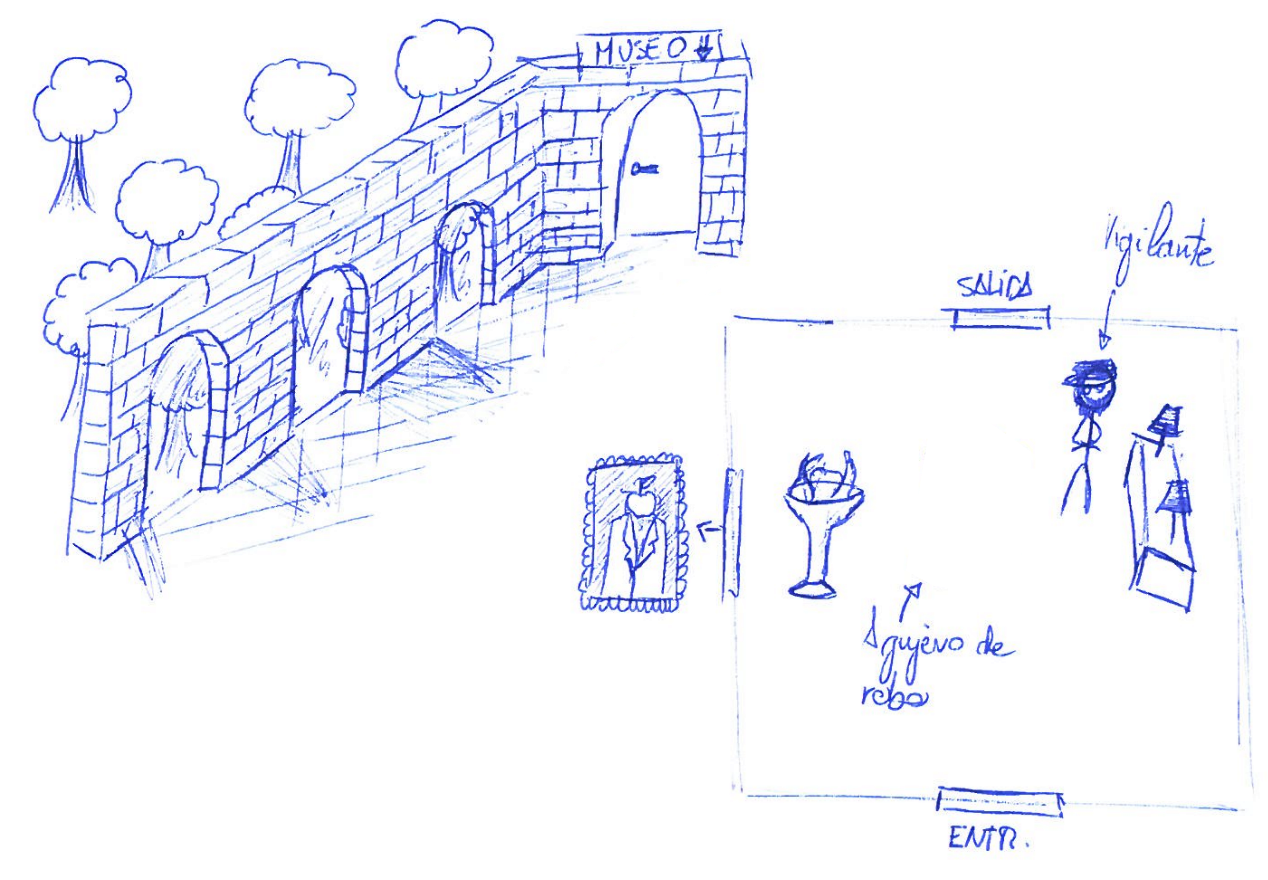
\includegraphics[width=.8\textwidth]{imagenes/7/bocetos/boceto-sala-0-1.png}
\caption{Boceto de la antesala y la sala de tutorial}
\label{fig:bocetos-salas-0-1}
\end{center}
\end{figure}

Una vez terminados los bocetos, se modeló la primera sala en Blender se comenzó a trabajar en importarla desde Unity, para lo que es necesario crear una Escena e importar en ella el archivo Blender desde el gestor de archivos. Una vez que lo hagamos, aparecerá como un \textbf{Prefab}\footnote{\url{https://docs.unity3d.com/es/current/Manual/Prefabs.html}}. De este modo, cuando el archivo Blender se modifique Unity lo detectará y actualizará su copia local, aunque por ser un Prefab no pueden modificarse desde Unity sin perder esta propiedad.

Actualmente, Blender cuenta con dos motores de renderizado; Blender Internal y Blender Cycles, y no son compatibles entre sí. Esto quiere decir que si por ejemplo creamos un material en Blender Internal y luego cambiamos a Cycles, éste no aparecerá. Aunque en teoría Unity trabaja mejor con los materiales de Blender Internal, al importarlos no aparecen como deberían y no pueden modificarse sus propiedades como su color, su \textit{metalicidad} o su mapa de normales, por lo que ha sido necesario rehacer todos los materiales de los modelos y volver a aplicarlos a mano.

Vamos a tomar como ejemplo una de las paredes de ladrillos para ver el flujo de trabajo de los materiales; tras modelarla, habría que descargar una textura para ella, para lo que se ha utilizado el sitio web \url{https://3dtextures.me/} que proporciona texturas procedurales gratuitas y con mapas de normales y rugosidad con licencia libre. Una vez hecho, se crea un material en Blender al que se le aplica la textura para ver cómo quedaría, aunque Blender Internal no da la opción de añadir más mapas a la textura. Tras esto, se importa el modelo a Unity y se crea un nuevo material, con la misma textura, al que se le añaden y configuran el resto de mapas.

La imagen \ref{fig:unity-sala-0} muestra el resultado final del modelado y la importación a Unity. Como el exterior con árboles, que puede verse a través de las ventanas, se reutiliza en otras salas se ha movido a una escena aparte que se importa cuando es necesario, recudiendo de este modo el peso de los modelos.

\begin{figure}[!h]
\begin{center}
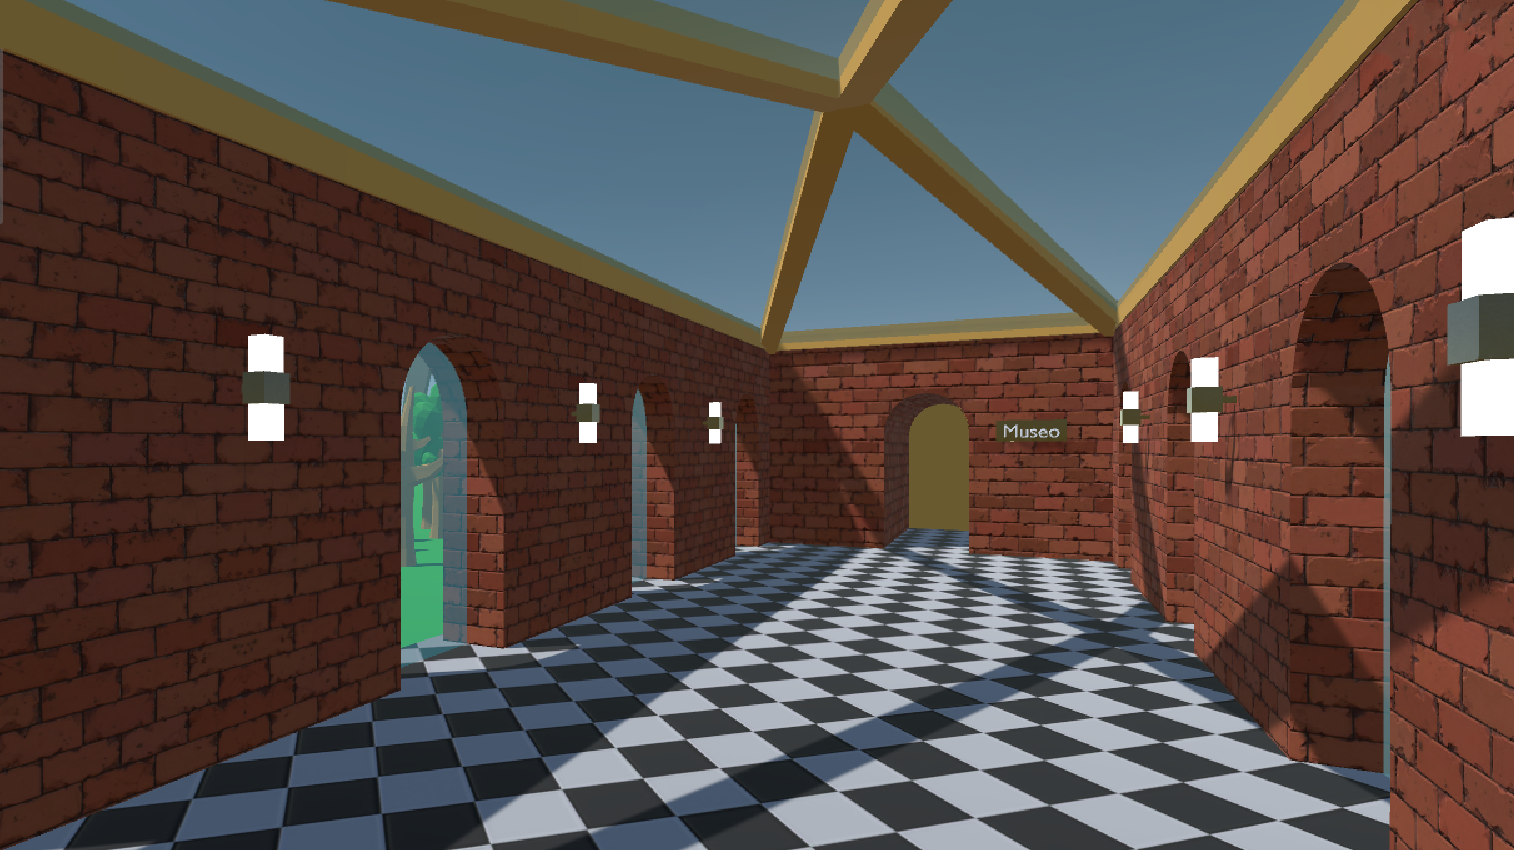
\includegraphics[width=0.85\textwidth]{imagenes/7/salas-unity/unity-sala-0.png}
\caption{Sala 0 vista desde Unity}
\label{fig:unity-sala-0}
\end{center}
\end{figure}

Tras ello se hizo lo mismo con la sala de tutorial, que puede verse en la figura \ref{fig:unity-sala-1}.

\begin{figure}[!h]
\begin{center}
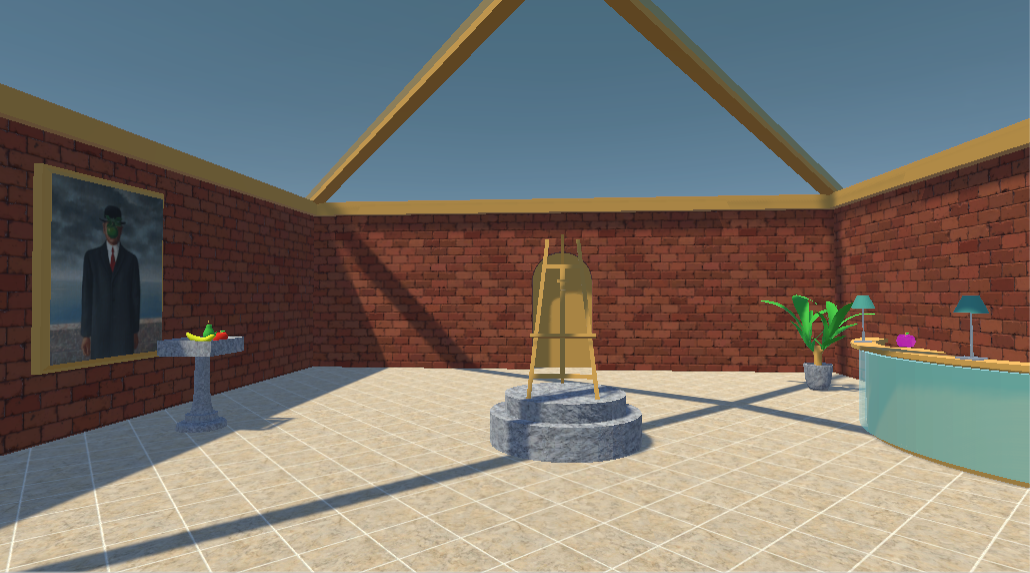
\includegraphics[width=0.85\textwidth]{imagenes/7/salas-unity/unity-sala-1.png}
\caption{Sala 1 vista desde Unity}
\label{fig:unity-sala-1}
\end{center}
\end{figure}

Además, aunque las cajas de colisiones automáticas de Unity funcionan bien para objetos no lo hacen para habitaciones, ya que estas cajas la rodean y no permiten detectar colisiones, por lo que ha sido necesario definir manualmente estas colisiones, para lo que se han utilizado los componentes \texttt{Box Collider} para cada una de la paredes, el techo y el suelo.

\subsection{Viajar entre salas}

Una vez que las dos salas estaban modeladas se trabajó en hacer que el jugador pudiera viajar entre ellas; por lo que se escribió un script en C\# que permitía viajar al jugador a otra sala al tocar una puerta, 

Para ello, lo primero que se hizo fue añadir una caja de colisiones a la puerta y activar la opción \texttt{Is trigger}, lo que le añade un \textit{listener} para poder activar otras funciones cuando detecte colisiones. Tras ello, se le añadió un componente tipo script, que puede verse simplificado en el listado \ref{lst:viajar-salas} que usa la clase \texttt{SceneManager} para cambiar la escena cuando el jugador colisiona con ella1. En él se declaran dos variables públicas para poder definirlas desde el propio inspector de Unity más cómodamente, como puede verse en la figura \ref{fig:door-teleporter-inspector}, lo que añade flexibilidad y realización al código.

\begin{lstlisting}[caption=Fragmento del script para viajar entre salas, label=lst:viajar-salas]
public string scene_name;
public float fadingTime = 10.0f;
public bool IsExitDoor = false;
    
private void OnTriggerEnter(Collider other)
{
    if (scene_name != "" && !SceneManager.GetSceneByName(scene_name).isLoaded)
    {
        SceneManager.LoadScene(scene_name, LoadSceneMode.Single);
    }
}
\end{lstlisting}

\begin{figure}[!h]
\begin{center}
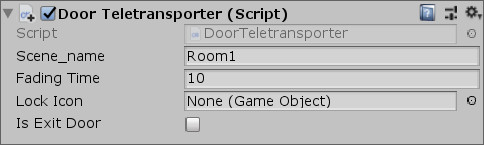
\includegraphics[width=0.6\textwidth]{imagenes/7/door-teleporter-inspector.jpg}
\caption{Script para cambiar de salas desde el inspector}
\label{fig:door-teleporter-inspector}
\end{center}
\end{figure}

Además, cada script puede implementar dos funciones, \texttt{Start()} y \texttt{Update()}, que se ejecutan automáticamente al inicio y en cada frame, respectivamente.

\subsection{Interacción con objetos virtuales}

Una vez modeladas las dos salas, se comenzó a trabajar en hacer que el jugador pudiera interactuar con los objetos virtuales. Al estar utilizando el framework \acs{VRTK} se han podido hacer uso de sus funciones para facilitar mucho el trabajo.

Lo primero que se hizo, tras modelar las tres piezas de fruta (una manzana, un plátano y una pera) fue dotarlas de físicas, para lo que se utilizaron los componentes \texttt{Box Collider} y \texttt{Rididbody}. Tras ello se hizo que interactuaran con los mandos del jugador con ayuda de los componentes \texttt{VRTK\_Interactable\_Object}, \texttt{VRTK\_Child\_Of\_Controller}, \texttt{VRTK\_Interact\_-} \texttt{Haptics} y se hizo que apareciera un borde amarillo cuando su caja de colisión detectara el mando con ayuda del componente \texttt{VRTK\_Outline\_Object\_-} \texttt{Highlighter}. Tras ello, se utilizó una \textit{snap drop zone} o zona en la que poder colocar objetos, para lo que se adaptó uno de los proporcionados por el framework.

Como resultado de esta entrega se generó el primer entregable y, por tanto, se grabó un vídeo presentando el proyecto y enseñando los avances, que puede verse en el siguiente enlace,

\begin{center}
    \url{https://youtu.be/m7rvcdZuUMI}
\end{center}


\section{Entrega 2}

\begin{figure}[!h]
\begin{center}
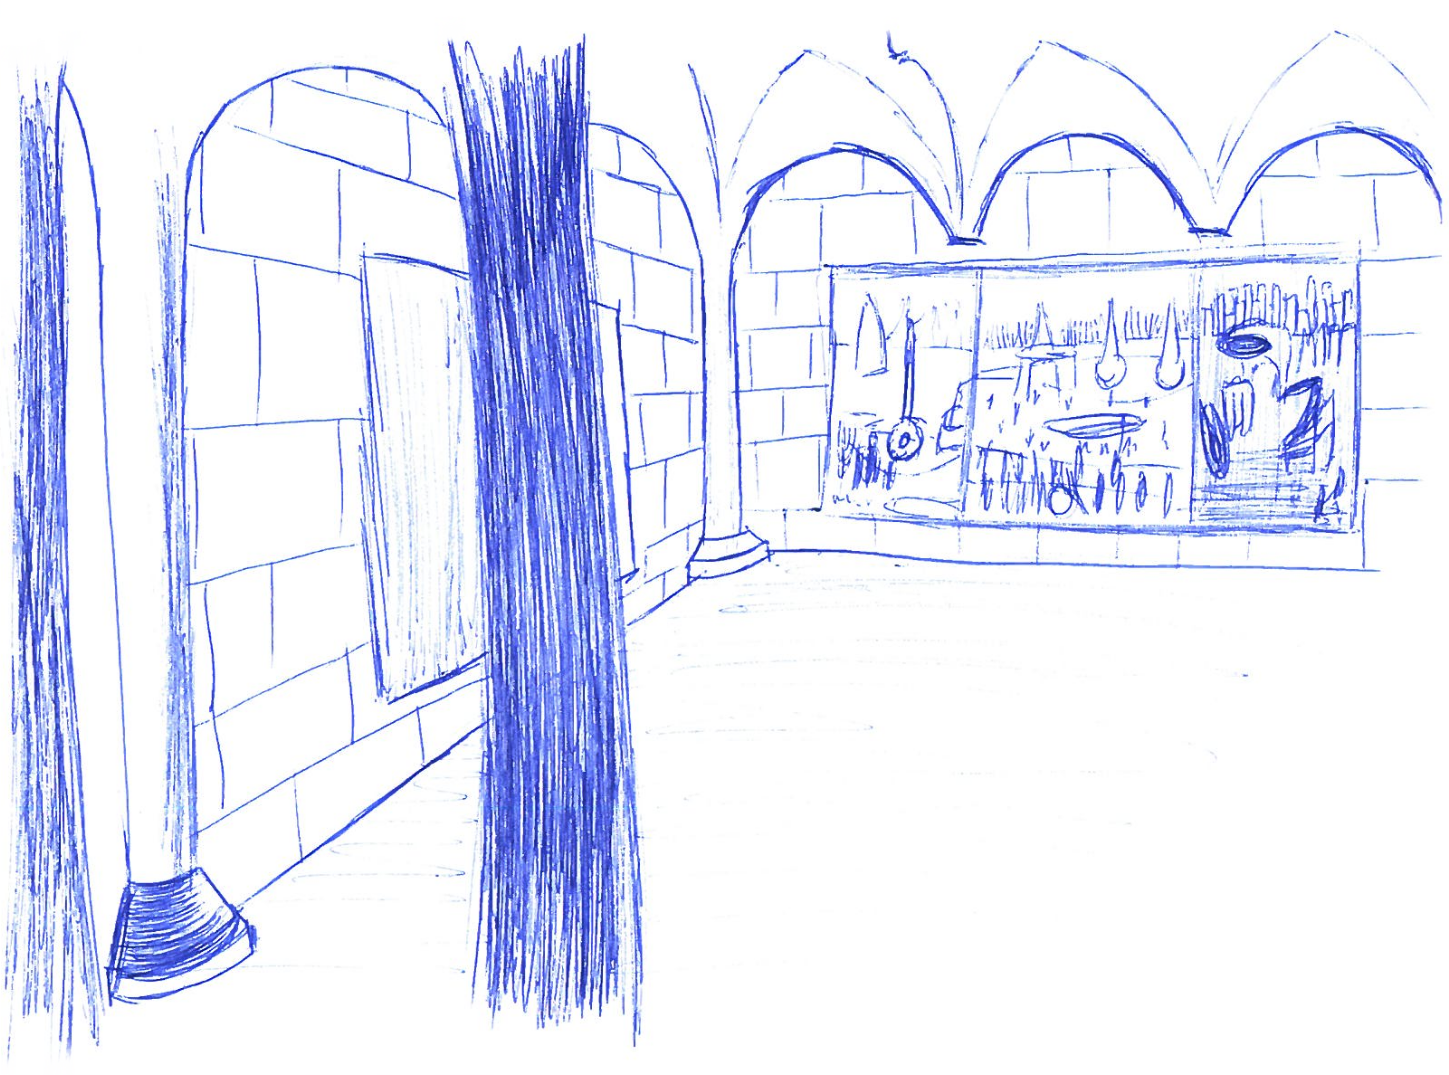
\includegraphics[width=1\textwidth]{imagenes/7/bocetos/boceto-sala-2.png}
\caption{Boceto de la segunda sala}
\label{fig:bocetos-salas-2}
\end{center}
\end{figure}

\section{Entrega 3}

\begin{figure}[!h]
\begin{center}
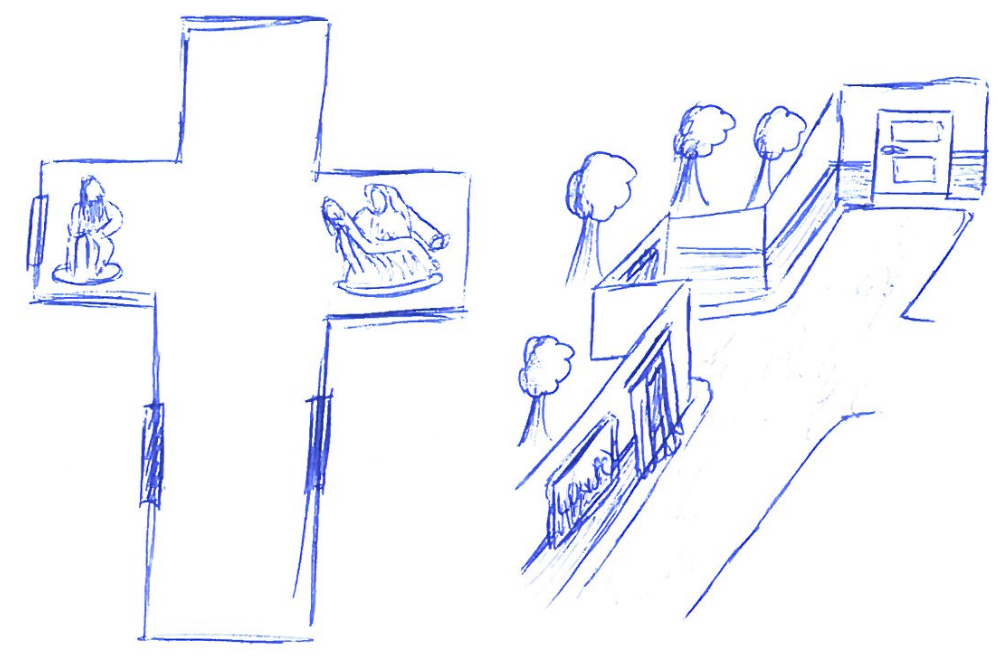
\includegraphics[width=1\textwidth]{imagenes/7/bocetos/boceto-sala-3.png}
\caption{Boceto de la tercera sala}
\label{fig:bocetos-salas-3}
\end{center}
\end{figure}

\section{Entrega 4}

\begin{figure}[!h]
\begin{center}
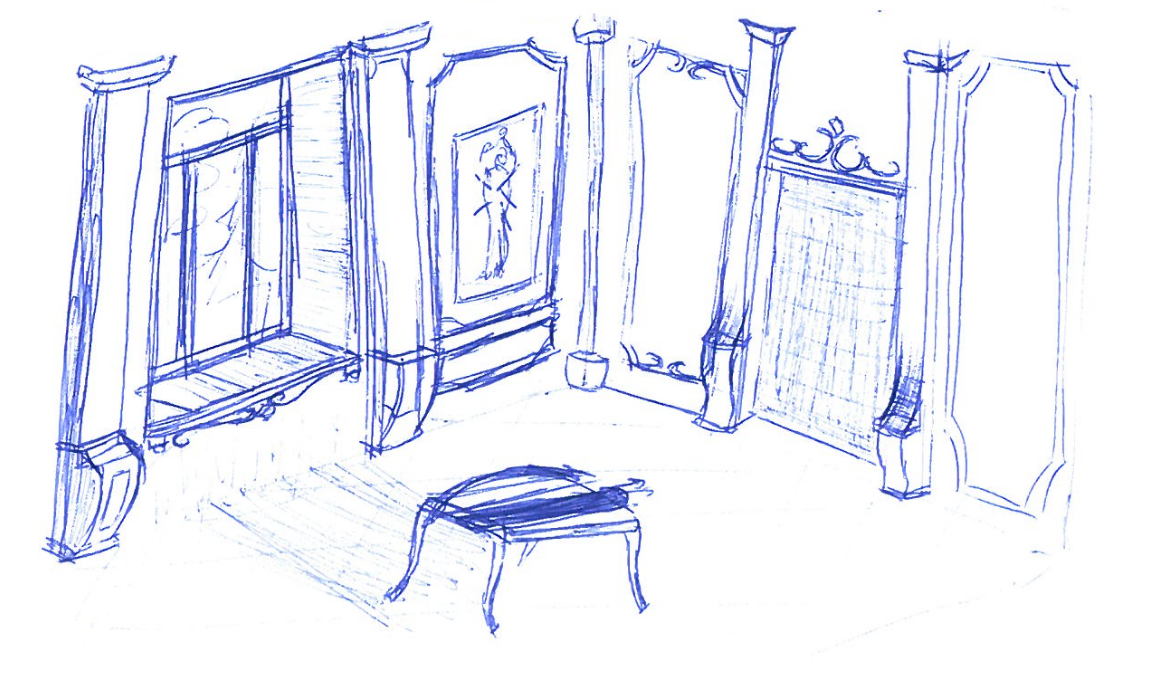
\includegraphics[width=1\textwidth]{imagenes/7/bocetos/boceto-sala-4.png}
\caption{Boceto de la cuarta sala}
\label{fig:bocetos-salas-4}
\end{center}
\end{figure}

\begin{figure}[!h]
\begin{center}
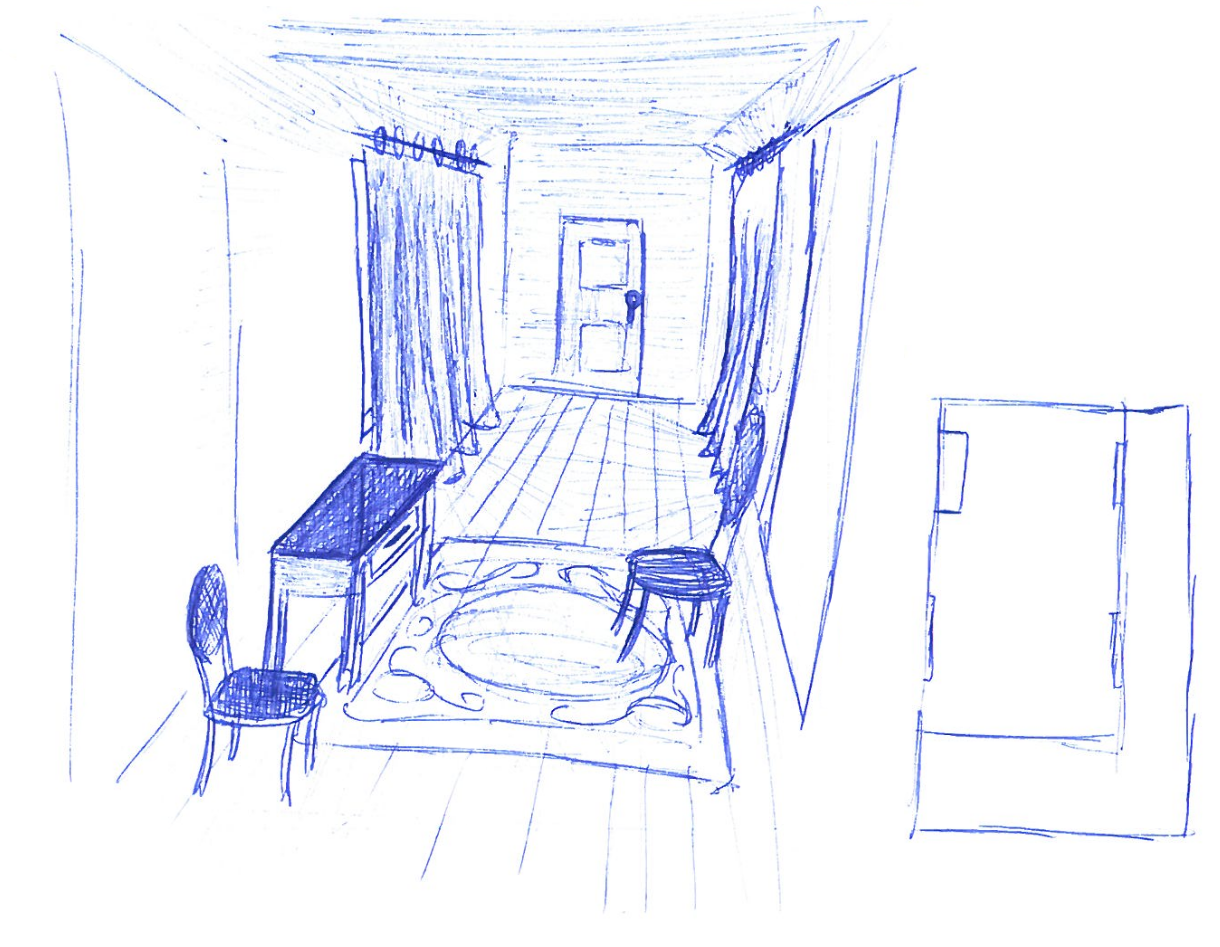
\includegraphics[width=1\textwidth]{imagenes/7/bocetos/boceto-sala-5.png}
\caption{Boceto de la quinta sala}
\label{fig:bocetos-salas-5}
\end{center}
\end{figure}

\section{Entrega 5}

\begin{figure}[!h]
\begin{center}
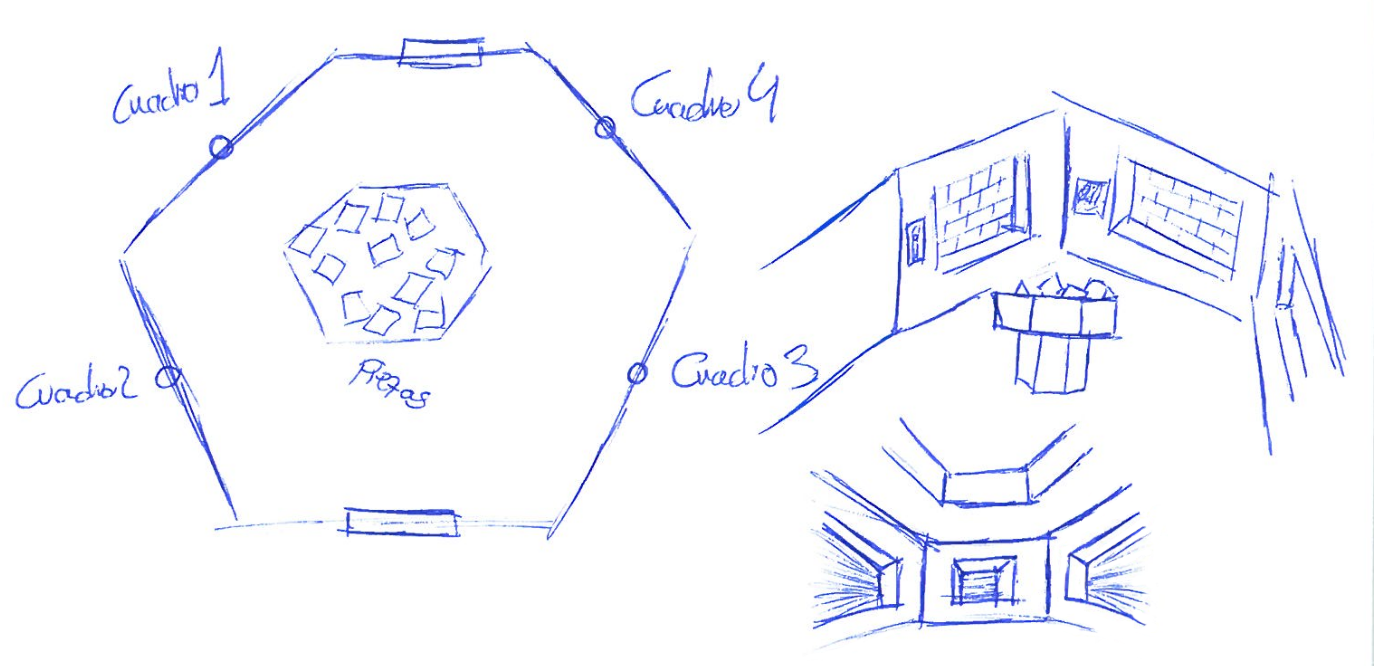
\includegraphics[width=1\textwidth]{imagenes/7/bocetos/boceto-sala-6.png}
\caption{Boceto de la sexta sala}
\label{fig:bocetos-salas-6}
\end{center}
\end{figure}

\section{Entrega 6}


\chapter{Conclusiones y Trabajo futuro}
\label{chap:conclusiones}

\section{Conclusiones}

\section{Trabajo futuro}

\chapter{Apéndices}
\label{chap:apendices}

\section{Apendice 1: Hola}


\nocite{*}
\bibliography{bibliografia/bibliografia}
\addcontentsline{toc}{chapter}{Bibliografía}
\bibliographystyle{apalike}


\end{document}
